\documentclass[12pt,oneside,openany,a4paper,%..... Layout
               afrikaans, english,%.............. Global language selection
	       ]{memoir}

\usepackage[masters-t,%.......................... Master thesis
            goldenblock,%........................ A5 type block (or a5block or wide)
	   ]{usthesis}%.......................... US thesis style with memoir

%
% PLEASE read the USthesis documentation for the class options
% and how to set line and paragraph spacing
%

%==== Language setup ================================================
\usepackage[latin1]{inputenc}%................... Recognizes ê, ë, etc
\usepackage{babel}%.............................. Language setup

%==== Math setup ====================================================
\usepackage{amsmath}%............................ Advanced math (before fonts)
\usepackage{amssymb}%............................ AMS Symbol fonts

%==== Font setup (default is Computer Modern) =======================
\usepackage[T1]{fontenc}%........................ Type 1 fonts
%\usepackage{fourier}
\usepackage{textcomp}%........................... Additional text character
\usepackage{bm}%................................. Bold math symbols (after fonts)

%==== Ref's, Bib's and Nomencl ======================================
\usepackage{usnomencl}%.......................... List of symbols (in usthesis pack)
\usepackage{usbib}%.............................. Bibliography    (in usthesis pack)
\bibliographystyle{usmeg-a}
\renewcommand\bibfont{\small}

%% For usmeg-a, the bib is a list of references. If you
%% are using usmeg-n comment out the following lines
\addto{\captionsafrikaans}{\renewcommand{\bibname}{Lys van Verwysings}}
\addto{\captionsenglish}{\renewcommand{\bibname}{List of References}}

%==== Graphics and Color ============================================
\usepackage{graphicx}%........................... Graphicx loaded in usthesis
\usepackage{color}%.............................. Color setup
\usepackage{eso-pic}%............................ Shipout commands for watermark
\newcommand*{\WaterMark}[2][0.15\paperwidth]{%
             \AddToShipoutPicture*{\AtTextCenter{%
             \parbox[c]{0pt}{\makebox[0pt][c]{%
             \includegraphics[width=#1]{#2}}}}}}

%==== Local Defs ====================================================
\makeatletter

%
% Please insert user defined commands here
% and NOT in the document itself!
%

\usepackage{siunitx}
\usepackage{caption}
\usepackage{subcaption}
\usepackage{url}
%\usepackage{gensymb}

\makeatother

%==== TITLE PAGE ====================================================
\title{\bfseries
\AorE{%-- Afrikaans ------------------------------------------
     (``Posisie en Ori\"{e}ntasie Afskatting van \'n Vierbeen Helikopter in die Buitelug)
    }{%-- English -------------------------------------------
        Pose Error Estimation of a Quadcopter in the Outdoors
}}

\author{JC Lock}{Jacobus C.\ Lock}
																			   
\degree{\AorE{MIng (Meg)}{MEng (Mech)}}
       {\AorE{Magister in Ingenieurswese (Megatroniese)}
             {Master of Engineering (Mechatronic)}}

\address{\AorE{%-- Afrikaans ----------------------------------------
               Departement Meganiese en Megatroniese Ingenieurswese,\\
               Universiteit van Stellenbosch,\\
               Privaatsak X1, Matieland 7602, Suid Afrika.%
             }{%-- English ------------------------------------------
               Department of Mechanical and Mechatronic Engineering,\\
               University of Stellenbosch,\\
               Private Bag X1, Matieland 7602, South Africa.
             }}
																		     
\faculty{\AorE{Fakulteit Ingenieurswese}%
              {Faculty of Engineering}}

\supervisor{Dr.\ WJ Smit}
\cosupervisor{Mr.\ J Treurnicht}

\setdate{11}{2015}
																     
%\SetSponsor{The financial assistance of the National Research Foundation (NRF)
%    towards this research is hereby acknowledged. Opinions expressed and
%    conclusions arrived at, are those of the author and are not necessarily to
%    be attributed to the NRF.}
																     
																     
%====================================================================
%     MAIN DOCUMENT
%====================================================================
\maxsecnumdepth{subsubsection}
\maxtocdepth{section}
															 
\begin{document}
														   
%==== Front matter ==================================================
\frontmatter
\WaterMark{UScrest-WM}
\TitlePage%
												    
\DeclarationDate{2015/10/27}
\DeclarationPage%
											  
\begin{abstract}[english]%===================================================
Vibrating a tillage tool is an effective way of reducing the draft force
required to pull it through the soil. The degree of draft force reduction is
dependent on the combination of operating parameters and soil conditions. It
is thus necessary to optimize the vibratory implement for different
conditions.

Numerical modelling is more flexible than experimental testing and analytical
models, and less costly than experimental testing. The Discrete Element
Method (DEM) was specifically developed for granular materials such as soils
and can be used to model a vibrating tillage tool for its design and
optimization. The goal was thus to evaluate the ability of DEM to model a
vibratory subsoiler and to investigate the cause of the draft force
reduction.

\end{abstract}

\begin{abstract}[afrikaans]%=================================================
Om `n tand implement te vibreer is `n effektiewe manier om die trekkrag, wat
benodig word om dit deur die grond te trek, te verminder. Die graad van krag
vermindering is afhanklik van die kombinasie van werks parameters en die
grond toestand. Dus is dit nodig om die vibrerende implement te optimeer vir
verskillende omstandighede.

Numeriese modulering is meer buigsaam en goedkoper as eksperimentele
opstellings en analitiese modelle. Die Diskrete Element Metode (DEM) was
spesifiek vir korrelrige materiaal, soos grond, ontwikkel en kan gebruik word
vir die modellering van `n vibrerende implement vir die ontwerp en optimering
daarvan. Die doel was dus om die vermoë van DEM om `n vibrerende skeurploeg
the modelleer, te evalueer, en om die oorsaak van die krag vermindering te
ondersoek.

\end{abstract}

\chapter{Acknowledgements}%==================================================

I would like to express my sincere gratitude to the following people

\chapter{Dedications}%=======================================================
\vfill
\begin{Afr}
  \begin{center}\itshape%
  Hierdie tesis word opgedra aan
  \end{center}
\end{Afr}
\vfill
\clearpage
	   
%============================================================================
\endinput

										     
\tableofcontents
\clearpage
									   
\setcounter{lofdepth}{2}
\listoffigures
\clearpage
							    
\listoftables
\clearpage
						  
%\include{frontmatter/Nomencl}
					     
%==== Main document =================================================
\mainmatter%
\setsecnumdepth{subsubsection}
%   \numberwithin{equation}{section}
%   \numberwithin{figure}{chapter}
%   \numberwithin{table}{chapter}

\chapter{Introduction}
\label{chap1}

\section{Problem Statement}
\label{sec:problem-statement}

Remote controlled model aeroplanes have been in use for decades and have been a favourite among hobbyists for almost equally long. However, the past decade has arguably seen the greatest increase in computing power and efficiency since the silicon transistor was first invented (refer to the law popularised by~\citeauthor{moore2005cramming}, \citeyear{moore2005cramming}). Thanks to the growth in the mobile technology industries, computers have not only grown more powerful, but also smaller, lighter, cheaper and more power efficient. The increase in computing power and decrease in size and cost have made it possible to place small computers onto a model aeroplane with the aim of having it autonomously control, or semi-autonomously assist in controlling, a model aeroplane. 

Coupled with the rise in mobile computing power, control theory has also reached a point where it has a better understanding of the unstable, underactuated plant, such as a Segway, and manages to stabilise and control plants like these in some cases. One case of interest is a multirotor unmanned aerial vehicle (UAV) which resembles a model helicopter with multiple rotors. The so-called quadcopter configuration is of special interest for this research project.  

Autonomous UAVs are typically fitted with a multitude of sensors that provide the control system with the orientation and localisation data of the UAV.\@ These sensors normally include an accelerometer, gyroscope and GPS, along with others such as a barometer, optic flow sensor, magnetometer, etc. In its semi-autonomous state, the control system uses the sensor readings to keep the UAV level and stable while following a human pilot's flight instructions. Optionally, the pilot can engage the UAV in \emph{mission} mode where the UAV autonomously completes a flight mission selected by the pilot without the pilot controlling it. A mission consists of a set of GPS coordinate waypoints and altitudes for the UAV to follow. The pilot can also set the UAV to \emph{loitering} mode, where the UAV's control system will keep the UAV stable and level while holding the UAV's yaw angle and position constant. 

A consequence of the smaller and lighter sensors UAVs are typically e\-quipped with is that they are often less accurate than their larger, more powerful counterparts. The implication this holds for UAVs in general can readily be observed from most UAVs in \emph{loiter} mode where there is often significant drift around the UAV's set point. The accuracy of the individual sensors are often known or can be determined, but due to the mathematical filtering and fusion of the different sensor readings, as well as other operations that the control system may perform on the sensor data, it is difficult to determine the resulting accuracy of the position and orientation measurements made by the UAV's sensor suite. As a result, the pose (a vector describing an object's position and orientation) estimation accuracy of an outdoor UAV is not yet known. This research project attempts to find and implement an affordable and reliable method to determine the pose estimation error of a typical quadcopter UAV.\@  

\section{Project Motivation}

For many years, UAVs have mostly been the playthings of hobbyists and the researchers studying them. In recent years, however, the improvements that have been made to UAVs, which include quad-, hexa- and octocopters, and their controllers have drawn the attention of large corporations, such as Amazon and DHL, have expressed interest in incorporating UAVs into their respective workforces. 

Similarly, national governments have also noticed the increasing commercial and industrial potential that UAVs have, while also recognising the dangers that they pose to society if left unregulated. As such, many governments have moved to regulate and place restrictions on how and where UAVs may be used. The general trend of the regulations, as demonstrated by the regulations released by the~\cite{sacaa-drone-regs}, is that UAVs may be manually flown by a pilot anywhere below an altitude of $\SI{120}{\m}$, $\SI{50}{\m}$ away from people and buildings and $\SI{10}{\km}$ away from any aerodrome. These regulations allow for autonomous UAV flight, provided the UAV remain within radio line of sight of a human operator that can manually take over control of the UAV at any time should something go wrong. 

At the moment, UAVs are not as safe as they should be and can pose a serious health hazard to their surroundings and people if handled incorrectly. This, coupled with a general lack of hardware- and software-based collision avoidance capabilities, makes aviation authorities very cautious about allowing fully autonomous flight (i.e.\ out of radio line of sight). There are many safety improvements that can be made to UAVs, such as an improved control strategy, hardware improvements (such as rotor shrouds) and other fail-safe and collision avoidance systems. 

Having accurate pose data of a UAV in flight available is crucial to implementing an effective control strategy and collision avoidance system. As mentioned in Section~\ref{sec:problem-statement}, UAVs do not estimate their own pose very well and are prone to sensor drift over time. This allows for a `bubble' of pose uncertainty to be drawn around a UAV in flight, where the true pose of a UAV will be somewhere within the bubble, but the true pose is indeterminable. If the bubble's volume can be determined, it will allow a UAV's control system to generate safer, more efficient flight paths, which will improve the UAVs performance and make them a more attractive and safe option for governments and industry. Furthermore, the measurement system can be used to evaluate and improve the flight performance of a UAV.\@ 

\section{Existing and Proposed Solutions}

The current state-of-the-art method in determining the pose of a UAV in flight is to use an indoor motion tracking system, such as a Vicon\footnote{www.vicon.com/} system which uses a set of infrared cameras to track markers placed on an object. However, such systems cannot be used in this case since the UAVs of interest to this project require access to their GPS coordinates. The GPSs used in this project require a strong connection with a reasonably clear line of site to at least 6 different GPS satellites to produce accurate position data. These GPSs are also low-powered and small and therefore struggle to make good connections to satellites when indoors. Their line of sight to the satellites will also be affected, further reducing the GPS's accuracy. It was therefore decided that the quadcopters would be flown in the outdoors for this project. This implies that an outdoor pose measurement system is required. 

Outdoor pose measurement systems, such as radar- or laser-based systems, can also be used to perform pose measurements of a UAV.\@ However, these systems normally come at a premium cost. It was therefore decided to investigate and implement another pose measurement method that is cheap, accurate, repeatable and easy to use. 

The proposed outdoor UAV pose measurement system is based on computer vision techniques where the pose data of an object can be extracted from image or video data containing the object. The system consists of a camera to capture the image data and a computer to perform the pose data extraction. 

\section{Project Objectives}

The objectives of this research project are as follows. 

\begin{itemize}
  \item Design and implement a relatively cheap computer vision pose measurement system.
  \item Determine the measurement accuracy of the computer vision system.
  \item Use the computer vision system to determine the pose estimation accuracy of a demonstration quadcopter in flight. 
\end{itemize}

\section{Document Structure}

This document begins with a review of existing literature and of previous research results in the fields relevant to this project, such as computer vision techniques, UAV control strategies and others. Afterwards, the design and implementation, as well as the determination of the accuracy of the computer vision pose estimation system is discussed. This is followed by a discussion on how the pose measurement error of the computer vision system was determined for subsequent measurements and used to determine the pose estimation accuracy of a quadcopter in flight. Finally, a conclusion on the significant findings and results, as well as shortcomings and potential improvements, are presented. 

\chapter{Literature Review}
\label{chap2}

\section{Introduction}

In this chapter, previous work and research findings relevant to this project are mentioned and discussed. These fields include the quadcopter platform, computer vision and machine learning techniques. Some concepts and terminology used in later chapters of this document are also explained and expanded upon.

\section{Quadcopters}

A quadcopter is an autonomous aerial vehicle (UAV) in a four-arm frame configuration. The frames typically come in an X or plus (+) shape with the control equipment and sensors located at the centre of the frame. Refer to Figure~\ref{fig:chap2-quad} for a picture of the Solar Thermal Energy Research Group's (STERG) Suncopter research platform which has an X configuration. They can also come equipped with either four or eight motors and props, though the four-rotor variant is commonly used and is used in this project.

\begin{figure}
  \centering
  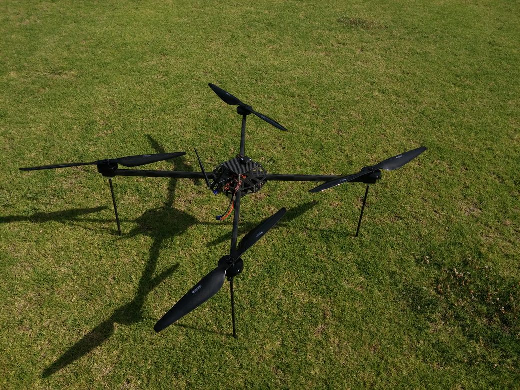
\includegraphics[clip, trim = 0 0 30 20, width=0.5\textwidth]{figures/chapter2/quadcopter}
  \caption[A picture of the Suncopter used by STERG.]{A picture of the Suncopter used by STERG.}
\label{fig:chap2-quad}
\end{figure}

Quadcopters move freely in three-dimensional space and have six degrees of freedom: three in position space ($x, y, z$) and three in orientation space ($\theta, \phi, \psi$), where the orientation is defined by the Eulerian aeroplane angle scheme, i.e.\ roll, pitch and yaw angles. The rotors on each axis of the frame rotate in the same direction and each axis' rotors spin in opposite directions relative to one another. Refer to Figure~\ref{fig:chap2-quad-rotation} for a diagram demonstrating this. 

\begin{figure}
  \centering
  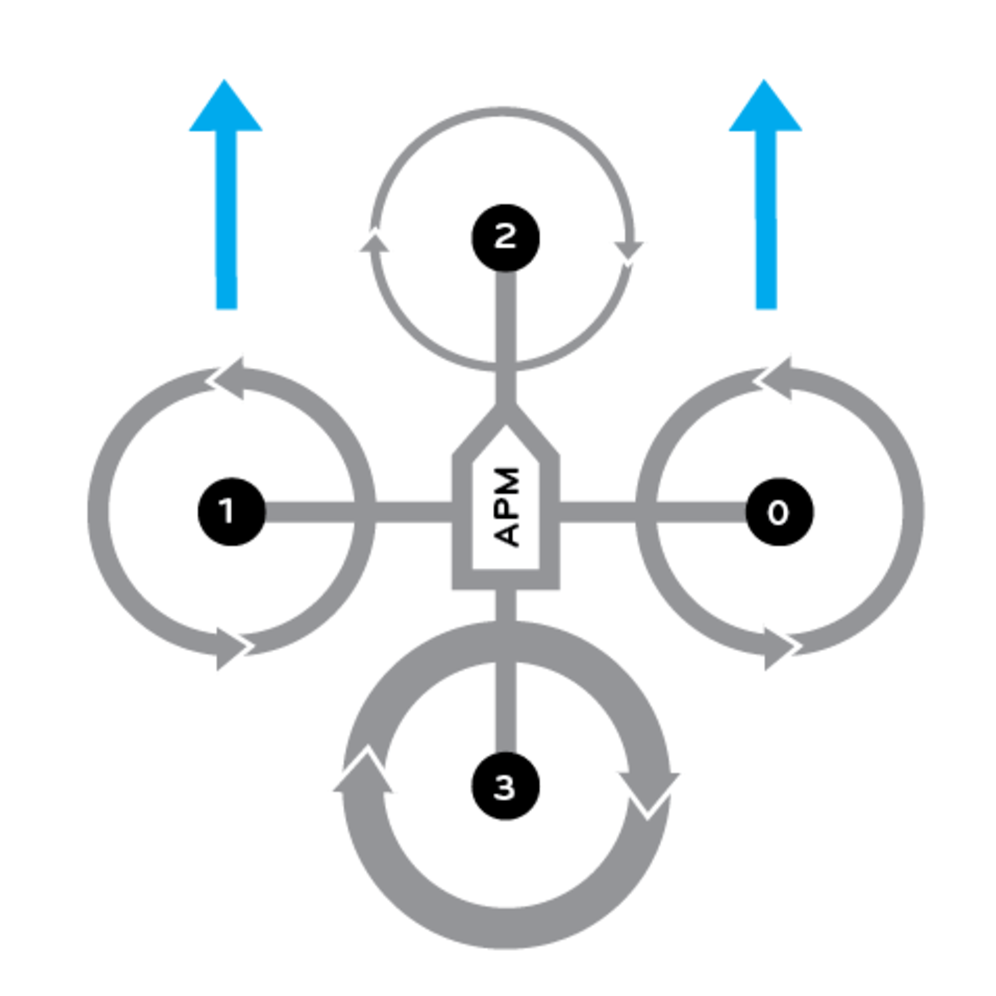
\includegraphics[width=0.5\textwidth]{figures/chapter2/quad_axis.pdf}
  \caption[Diagram presenting the opposing axis rotations directions.]{A diagram presenting the opposing axis rotation directions. The thickness of the arrows represent the power output of the motor~\citep{quad-rotation-pic}.}
\label{fig:chap2-quad-rotation}
\end{figure}

Movement in each of the six dimensions is described below. 

\begin{enumerate}
  \item Forward/backward or left/right movement: Keep one axis' rotor speed constant, while raising or lowering the speed of the rotors on the other axis (shown in Figure~\ref{fig:chap2-quad-rotation}).
  \item Higher/lower: Increase or decrease all of the rotor speeds.
  \item Roll/pitch: Linear movement is achieved by tilting the quadcopter, therefore movement in the roll and pitch dimensions is achieved with the same process as described in the first point. 
  \item Yaw: Increase or decrease the rotor speed of one axis relative to the other. 
\end{enumerate}

As described in Chapter~\ref{chap1}, the goal of this project is to determine a quadcopter's pose estimation error, i.e.\ the difference between a quadcopter's true pose and its estimated pose. To be able to do this, it is important that the dynamics and control strategies of a typical quadcopter are well defined and understood. This section sets out to discuss the work that has gone into the dynamic modelling of a quadcopter, as well as the different control strategies that have been developed and implemented in the past. 

\subsection{Quadcopter Modelling}

When designing a control system, arguably the most crucial part of the design process is to derive an accurate mathematical model of the plant, since an accurate plant model will lead to more stable response and superior performance. The plant in this case is a UAV in a quadcopter configuration. 

As part of their X-4 Flyer project,~\cite{hamel2002dynamic} set out to derive a simple model for their plant using only rigid body dynamics and abstract force and torque actuators. As stated by~\cite{Pounds2010c}, this model (like many others that were derived at the time) represents the quadcopter as a rigid body mass with inertia and autogyroscopics, which is only affected by gravity and actuator torques.~\citeauthor{Pounds2010c} further argue that these simple quadcopter models do not accurately represent the complex helicopter-like behaviour exhibited by real quadcopters at high rotor speeds. The high-speed rotor effects include blade flapping effects, which affect the quadcopter frame's oscillatory modes, rotor flapping introduced by varying a quadcopter's yaw angle and variable airflow velocities over the rotor blades caused by changing roll and pitch angles.

In an attempt to create a more accurate quadcopter model that will allow a quadcopter to be more controllable at high rotor speeds,~\citeauthor{Pounds2010c} set out to derive a model incorporating rigid body dynamics as well as the aerodynamic effects mentioned earlier. Their model is based, in part, on the diagram given in Figure~\ref{fig:chap2-quad-model}.

\begin{figure}
  \centering
  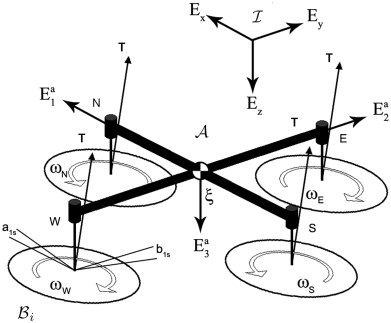
\includegraphics[width=0.5\textwidth]{figures/chapter2/pounds_quad-model.jpg}
  \caption[Diagram of the quadcopter model.]{A diagram of the quadcopter model which includes the blade flapping dynamics discussed by~\cite{Pounds2010c}.}
\label{fig:chap2-quad-model}
\end{figure}

Their resulting model was used to develop a simple Proportional Integral Differential (PID) attitude and altitude controller for the purpose of model verification. Their results show that the quadcopter stabilised itself (in indoor flight) with a level of precision of $\pm\ang{1}$, and $\pm\ang{5}$ during outdoor flight. The lower precision during outdoor flight is due to the added wind disturbances and sensor drift. They therefore conclude that their model is sufficiently accurate to safely control a quadcopter for hovering. However, they did not compare their more complex model against the model of~\citeauthor{hamel2002dynamic}, which is based solely on rigid body dynamics. 

\subsection{Control Strategies}

After an accurate model has been established, the next important part of designing a good control system is the controller itself. Many controllers have been implemented and tested on quadcopters over the years and different control strategies have also been investigated. Some of the most prevalent control strategies and controllers are discussed here.

\subsubsection{Indoor vs. Outdoor Control}

There are different types of quadcopters, with each of them equipped with different sensors and equipment. However, two types of quadcopters with distinctly different sensor and control approaches are relevant to this project. These are indoor and outdoor quadcopters and each of them work in different ways and implement very different control schemes. 

To help with stability control, indoor quadcopters may or may not come equipped with an on-board inertial measurement unit (IMU), which typically includes an accelerometer and a gyroscope. However, they commonly solely rely on an external motion detection system which tracks the quadcopter's movement and provides position and orientation feedback to the controller, thereby closing the control loop. These quadcopters can be very accurate due to the highly accurate external motion sensing equipment which are capable of sub-millimetre levels of accuracy~\citep{richards1999measurement}. As a result they are capable of performing remarkable acrobatic feats. However, these systems are restricted to carefully regulated and controlled indoor environments.

Outdoor quadcopters do not have the luxury of highly accurate external motion tracking systems and have to rely on their on-board sensors to provide the controller with pose feedback. A quadcopter's on-board sensor suite may vary between quadcopter platforms; however, they almost certainly come equipped with an IMU to provide pose data, but since the IMU readings for position data drifts with time due to integration errors, a GPS sensor is added to provide a base-line reading of a quadcopter's position. Other sensors that may be included are magnetometers, barometers, visual feedback sensors and sonar sensors. To combine the readings of the different sensors a filtering technique, such as an Extended Kalmann Filter, can be used. The pose estimation error of the combination of the different readings are, in theory, less than the most accurate sensor in the suite, but this has not yet been proven and the exact error margin is yet to be determined. 

\subsubsection{Hover Control}

Hover control refers to a quadcopter's ability to hover and remain stable at a set point in three-dimensional space. The stable hovering of a quadcopter has been the focus of many projects and research papers in the past 15 years. As a result, many different control methods and schemes have been investigated, implemented and compared. 

\cite{bouabdallah2004pid}, as part of their OS4 project, compared the modern linear quadratic regulator (LQR) and classic PID controller, with respect to the control performance (disturbance rejection, reference tracking, etc.) of a quadcopter.

They found that the PID controller produced better results than the LQR in terms of reference tracking and dynamic performance. This is a surprising result, since LQR controllers normally excel at controlling an unstable, underactuated plant such as a quadcopter platform. They suspect that the reason for this surprising result is that they neglected the effects of actuator dynamics, such as blade and rotor flapping, in their quadcopter model and the PID was better at handling plant uncertainties. They expect that an LQR controller will outperform a PID controller if a more accurate model is used which takes aerodynamic effects into account. 

Some researchers have also investigated controlling a quadcopter using an H-infinity (H$_{\inf}$) control structure and a model predictive controller (MPC). Most notably,~\cite{raffo2010integral} have done extensive research on this topic. MPCs are modern computationally efficient controllers that drive a plant's state to a reference state within predefined constraints (eg.\ motor saturation, model dynamics, etc.), while a properly designed, non-linear H$_{\inf}$ controller is very good at rejecting disturbances (eg.\ wind gusts, motor vibrations, etc.) and are robust to model uncertainties. They opted to combine the two controllers in an intelligent manner to extract the best performance from their quadcopter. 

In their simulations, they found that the resulting controller exhibited good performance characteristics; presenting good reference tracking, proving to be robust with uncertain mass and inertia terms and deals well with disturbances on all six degrees of freedom at different points in time. However, they are yet to implement their controller configuration on a real quadcopter. Although the algorithms and methods they used are computationally efficient, it may still prove to be too computationally intensive for the limited computing power on-board a UAV.\@ Given the fast growth of processing power, however, this controller configuration may become a more viable option in the near future. 

Controllers for enabling a quadcopter to hover have already been successfully designed and implemented, and it is therefore possible to stabilise and accurately control a quadcopter for hovering operations. 

\section{Computer Vision}

Computer vision is a diverse field which primarily focuses on finding methods for acquiring, processing, analysing and understanding images captured of the world. The `world' in this context refers to the three-dimensional world as perceived by living beings. There are many sub-fields of research, but a common theme across all of them is to make a computer mimic the human ability to perceive and understand an image and elicit an appropriate response to different visual inputs. 

The fields of interest for this project are feature detection, feature tracking and pose estimation. This section discusses the work that has been performed in these fields of research.  

\subsection{Camera Matrix}

A digital image is a collection of two-dimensional colour intensity vectors representing a collection of three-dimensional space vectors. These collections of vectors are related by a matrix, $C$, known as the camera matrix. The camera matrix contains the intrinsic parameters of the camera that recorded the image, i.e.\ the focal lengths and principle point of the camera, as well as the extrinsic, or pose, parameters of the camera, i.e.\ the camera's position and orientation information. The camera matrix, $C$, as derived by~\cite{heikkila1997four}, is 

\begin{equation}
  \label{eq:chap2-cam-matrix}
  C = 
  NP.
\end{equation}
The matrix $N$ in Equation~\ref{eq:chap2-cam-matrix} is given by

\begin{equation}
  \label{eq:chap2-cam-intrinsic}
  N = 
  \begin{bmatrix}
    f_x & 0   & u_0 \\
    0   & f_y & v_0 \\
    0   & 0   & 1   \\
  \end{bmatrix}.
\end{equation}
Here, $f_x$ and $f_y$ describe the focal lengths of the camera, while $u_0$ and $v_0$ represent the camera's principal point coordinates. The principal point, also known as the focal point, is where the camera's axis crosses the image plane and is ideally situated in the centre of the camera lens. However, due to manufacturing defects, this is rarely the case. Refer to Figure~\ref{fig:chap2-focal} to see what the focal length and principle point coordinates represent. 

\begin{figure}
  \centering
  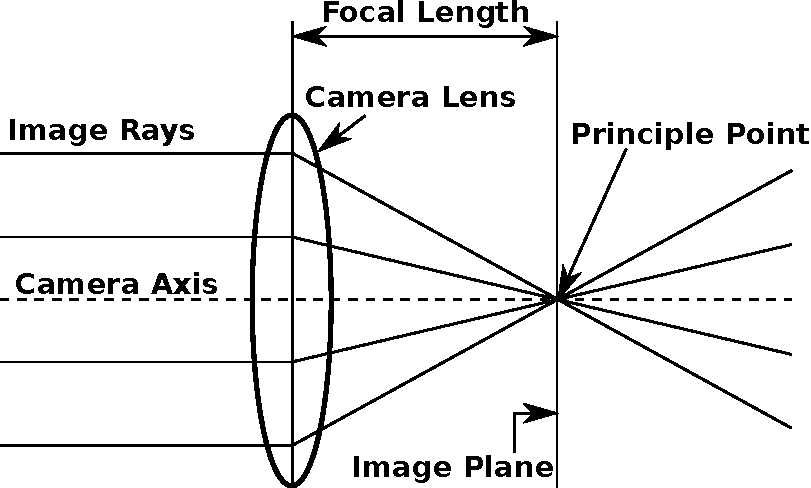
\includegraphics[width=0.6\textwidth]{figures/chapter2/focal_details}
  \caption{Diagram showing what the focal length and principle point parameters represent. }
\label{fig:chap2-focal}
\end{figure}

The pose matrix, $P$, from Equation~\ref{eq:chap2-cam-matrix} is given by

\begin{equation}
  \label{eq:chap2-cam-extrinsic}
  P = 
  \begin{bmatrix}
    R | \bm{T}
  \end{bmatrix}
  =
  \begin{bmatrix}
    r_{11} & r_{21} & r_{31} & t_1 \\
    r_{21} & r_{22} & r_{32} & t_2 \\
    r_{31} & r_{23} & r_{33} & t_3 \\
  \end{bmatrix}.
\end{equation}
In the matrix $P$, $R$ is a $3\times3$ cell matrix describing the orientation of the camera and $\bm{T}$ is a three-dimensional vector describing the position of the camera. The pose information in $P$ is given relative to some reference object or plane. 

The two-dimensional image projection of an object in three-dimensional world space is related through $C$ with the relation given in Equation~\ref{eq:chap2-2d-to-3d}. The camera matrix is commonly determined through some camera calibration procedure. One such a procedure is discussed in Section~\ref{sec:chap2-cam-calibration}.

\begin{equation}
  \label{eq:chap2-2d-to-3d}
  \bm{x}_c
  = C
  \bm{X}_w
\end{equation}
In Equation~\ref{eq:chap2-2d-to-3d}, $\bm{x}_c$ is a homogeneous image vector $[x\;y\;1]$ and $\bm{X}_w$ is a homogeneous world coordinate vector $[X\;Y\;Z\;1]$. 

\subsection{Camera Calibration}
\label{sec:chap2-cam-calibration}

A properly calibrated camera is an important part of any computer vision system, since the accuracy of the data extracted from an image strongly depends on the accuracy of the calibration procedure and results. The goal of the calibration procedure is to produce the matrix $C$ (as given in Equation~\ref{eq:chap2-cam-matrix}), as well as finding the camera's distortion coefficients introduced by low-quality or fish-eye lenses. There are various camera calibration procedures available: from the two-step calibration described by~\cite{melen1994geometrical} to the classical approach given by~\cite{slama1980manual} where a non-linear error function is minimised. However, the minimisation problem presented by~\citeauthor{slama1980manual} is computationally inefficient and slow, while~\citeauthor{melen1994geometrical}'s method does not account for image distortion and correction. A popular calibration method is the four-step method proposed by~\cite{heikkila1997four} as an extension to the two-step method which was the prevalent calibration procedure at the time.

The \emph{calibrateCamera()} function of the OpenCV\footnote{Open-source computer vision library, OpenCV v2.4.8. Source-code available at github.com/Itseez/opencv} computer vision library \citep{bradski2000opencv} makes use of the four-step method. The details of this method is beyond the scope of this research project, however, a broad overview of the steps and equipment required to calibrate a camera is provided. 

To perform the calibration and find the camera matrix, OpenCV requires two sets of data: one two-dimensional image data set, $\bm{x}_c$, as well as a set of corresponding three-dimensional data points, $\bm{X}_w$. This implies that image data of an object, where the dimensions and coordinates of certain features are known, must be recorded. In practice, any well-characterised object can be used for calibration. For example, some calibration methods rely on a three-dimensional cube covered in precisely laid out markers. However, since manufacturing and distributing such precisely constructed objects to a large audience is infeasible, OpenCV opts to use a more convenient flat, regular pattern, such as chessboard or asymmetrical dot pattern. Figure~\ref{fig:chap2-calib-pattern} shows an example of a typical chessboard pattern generated by OpenCV.\@ With this flat pattern, the features used to populate the data sets would be the corners on the chessboard, i.e.\ where one black block meets another black block. The drawback to this approach, however, is that multiple views of the flat calibration pattern are required, whereas a single image of a three-dimensional object would suffice. However, more data points would allow the optimisation procedure built into the algorithm to find a more accurate result.  

\begin{figure}
  \centering
  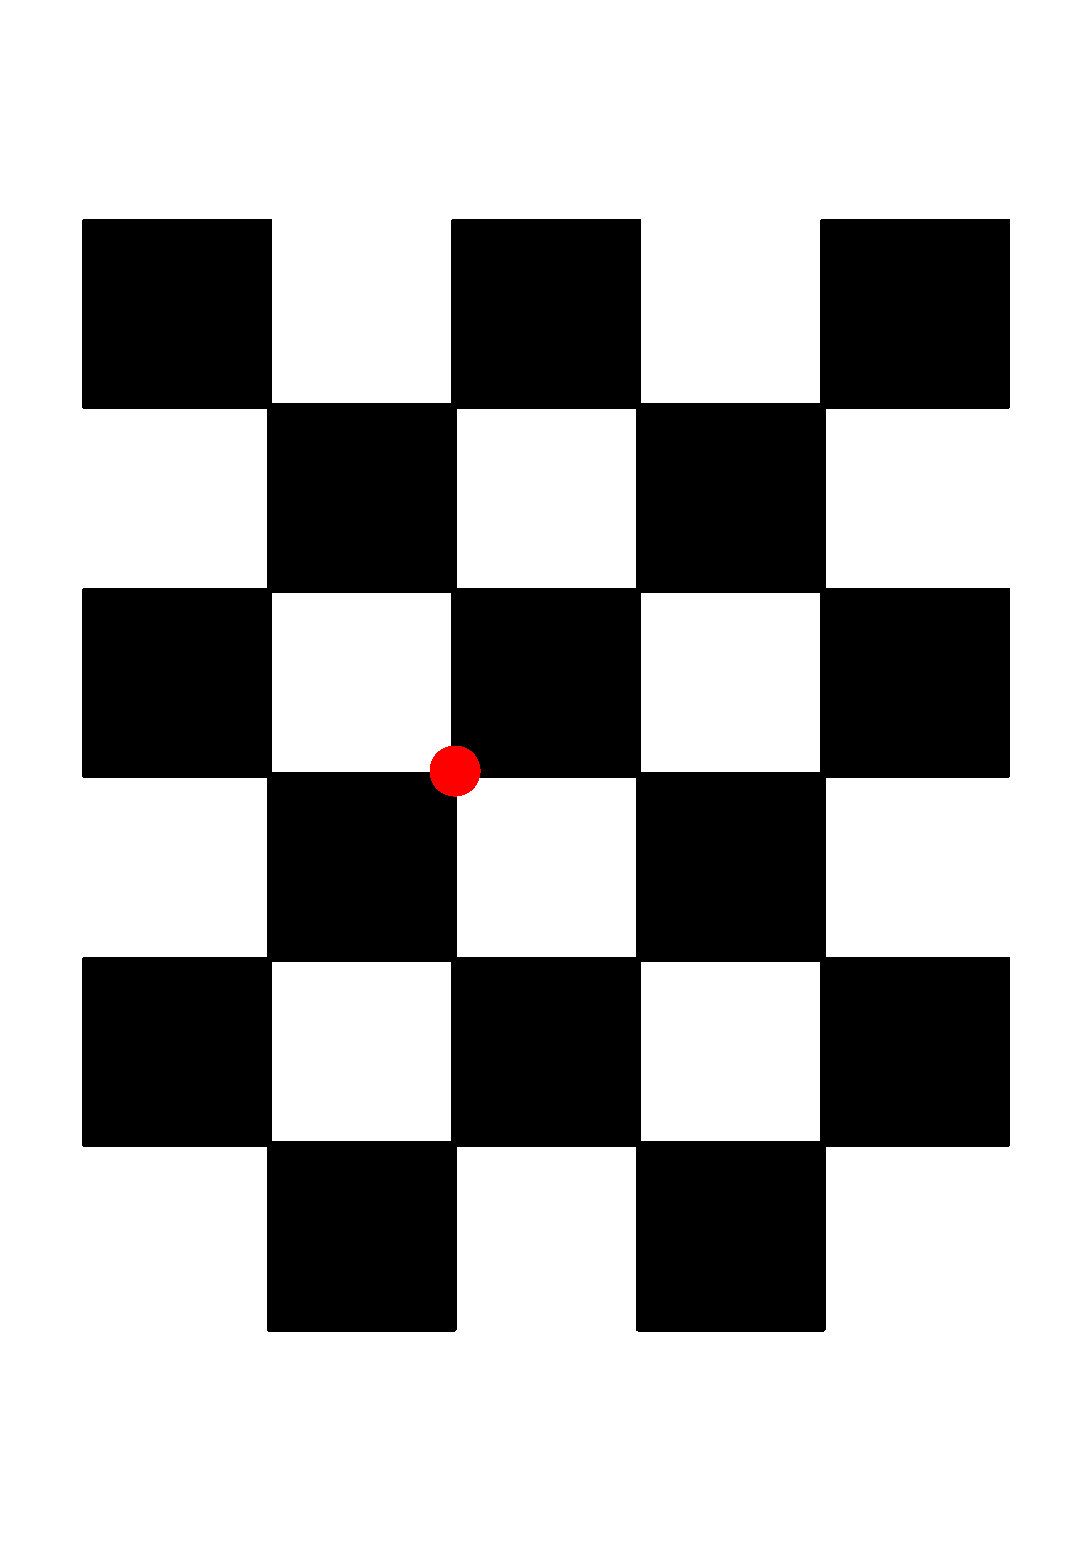
\includegraphics[angle=90, width=0.5\textwidth]{figures/chapter2/chessboard_pattern}
  \caption{An example of a typical chessboard pattern used for calibration.}
\label{fig:chap2-calib-pattern}
\end{figure}

In the case of the chessboard pattern, acquiring the two-dimensional pixel coordinates of the corners is accomplished by using OpenCV's \emph{findChessboardCorners()} and \emph{findCornerSubPix()} functions, which make use of the corner detection algorithm described by~\cite{harris1988combined}. The three-dimensional world coordinates of the features are fed into the calibration function according to an axis-system and measurement unit defined by the programmer. These coordinates can be as simple as a vector containing the feature coordinates in square units, where, for example, the corner from Figure~\ref{fig:chap2-calib-pattern} will be represented as $(3, 2, 0, 1)$ in homogeneous coordinates (note that $z$ will be zero since the board is flat). 

For the best calibration results, OpenCV recommends that camera calibration takes place within a well-lit room with a white background, using a calibration pattern with a wide white border in clear view of the camera and at different positions and orientations relative to the camera. These recommendations are mainly to increase the contrast between the black features and the white background on the calibration pattern and make it easier for OpenCV to accurately find each feature's pixel coordinates. Furthermore, the more diverse the position and orientation data is, the more accurate the estimate for the intrinsic camera parameters will be. 

Once the two-dimensional and three-dimensional data sets are known, Open\-CV's \emph{calibrateCamera()} function can determine the camera matrix, $C$. 

\subsection{Principle n-Points Problem}

The Principle n-Points (PnP) problem, as stated by~\cite{horaud1989analytic}, `is the problem of finding the position and orientation of a camera with respect to a scene object from $n$ correspondence points', where the scene object would normally be a well-characterised calibration object or pattern. It is a well-researched sub-field of computer vision with different solutions to the problem that have been proposed. They include some non-iterative solutions, such as the P3P solution proposed by~\cite{gao2003complete} and the PnP solution by~\cite{lepetit2009epnp} and~\cite{schweighofer2006robust}, and iterative solutions such as the method proposed by~\cite{lu2000fast}.

It was found that iterative methods produce very accurate results, but can become unstable if it is not properly initialised and can take a long time to converge. Conversely, the non-iterative ePnP method by~\citeauthor{lepetit2009epnp} implements~\citeauthor{schweighofer2006robust}'s robust solver and produces results whose accuracy is comparable to those produced by its iterative counterpart. However, it produces these results in a fraction of the time, having a big-$\mathcal{O}$ complexity that grows linearly ($\mathcal{O}(n)$), as opposed to competing non-iterative methods which commonly have a big-$\mathcal{O}$ complexity in the order of 4 or more ($\mathcal{O}(n^4)$). Unfortunately, the accuracy of the ePnP method's results are fairly dependant on the number of sample points, i.e.\ the number of feature correspondences between the three-dimensional features and their two-dimensional projections. 

The OpenCV library has implementations of both the P3P and ePnP methods, as well as its own solution based on Levenberg-Marquardt optimisation, as described by~\cite{levenberg1944method} and~\cite{marquardt1963algorithm}, where the pose that minimises the reprojection error - that is the sum of the squared distances between the actual two-dimensional points and the projected two-dimensional points - is determined and selected~\citep{opencv-levenberg}. 

OpenCV's \emph{solvePnP()} function can be used to determine the pose of a camera relative to a calibration pattern. This can be accomplished as follows. During the camera calibration procedure, the intrinsic parameter matrix, $N$, of Equation~\ref{eq:chap2-cam-intrinsic} is determined. Then, using a calibration pattern, a set of three-dimensional feature coordinates and their corresponding two-dimensional projection is obtained. Following from Equation~\ref{eq:chap2-2d-to-3d}, with the matrix $C$, the two-dimensional image projection vector, $\bm{x}_c$, and the three-dimensional object coordinate vector, $\bm{X}_w$, the pose matrix, $P$, can be found. This matrix contains the position and orientation data for the camera relative to the calibration pattern. 

\subsection{Random Sample Consensus}

For both the camera calibration and PnP solving functions, two-dimensional image projection data of a three-dimensional object is required. As mentioned, OpenCV's \emph{findChessboardCorners()} function can automatically detect corner features on a chessboard pattern and provide the two-dimensional projection data. However, the methods employed are prone to erroneously classifying some features as corners, introducing unwanted noise into the system. 

To remedy this,~\cite{fischler1981random} proposed a new algorithm to iterate through a data set and reject any outlier data. This algorithm is known as RAndom SAmple Consensus (RANSAC) and is commonly used in the computer vision field to determine if an image feature, e.g.\ a corner on a chessboard, has been classified correctly and rejecting it if it was not, thereby reducing the amount of noise in a data set. 

\section{Machine Learning}

Machine learning is a research field in computer science with strong ties to the fields of mathematical statistics and optimisation. The field is well-es\-tab\-lished and has its roots with a paper by~\cite{turing1950computing} in which he poses the question, `Can machines think?'.~\cite{michalski2013machine} offers a somewhat more formal definition: `A computer program is said to learn from experience E with respect to some class of tasks T and performance measure P, if its performance at tasks in T, as measured by P, improves with experience E'. This means that researchers in the machine learning field are attempting to find efficient methods and algorithms that will allow a computer to be trained to make intelligent decisions when presented with an arbitrary input data set. 

An everyday example of a system that uses machine learning is the face detection software that often come packaged with digital cameras. Here, the camera has been trained to search for facial information within the image, and consequently detects them when presented with other images containing faces.

Various machine learning algorithms and types have been developed, each of them having their unique advantages and limitations. Here, brief discussions on the most prevalent machine learning methods are provided. 

\subsection{Artificial Neural Networks}

Artificial neural networks (ANNs) are a family of machine learning algorithms which have seen a rise in popularity in recent years. The idea behind ANNs is to model the vast network of interconnected neurons in a biological brain in such a way that the network can be trained to recognise patterns and make decisions based on what it perceives, much like any animal or human would. 

Normally, an ANN consists of a multitude of artificial `neurons', or nodes, numbering anything between a handful to many millions, arranged in a series of layers. Each of the nodes in every layer is connected to each other node in the layers on either side of it, forming a vast network of interconnected nodes forming something analogous to a living brain. A diagram of the layout of a simple feed-forward ANN is given in Figure~\ref{fig:chap2-ann-layout}.

\begin{figure}
  \centering
  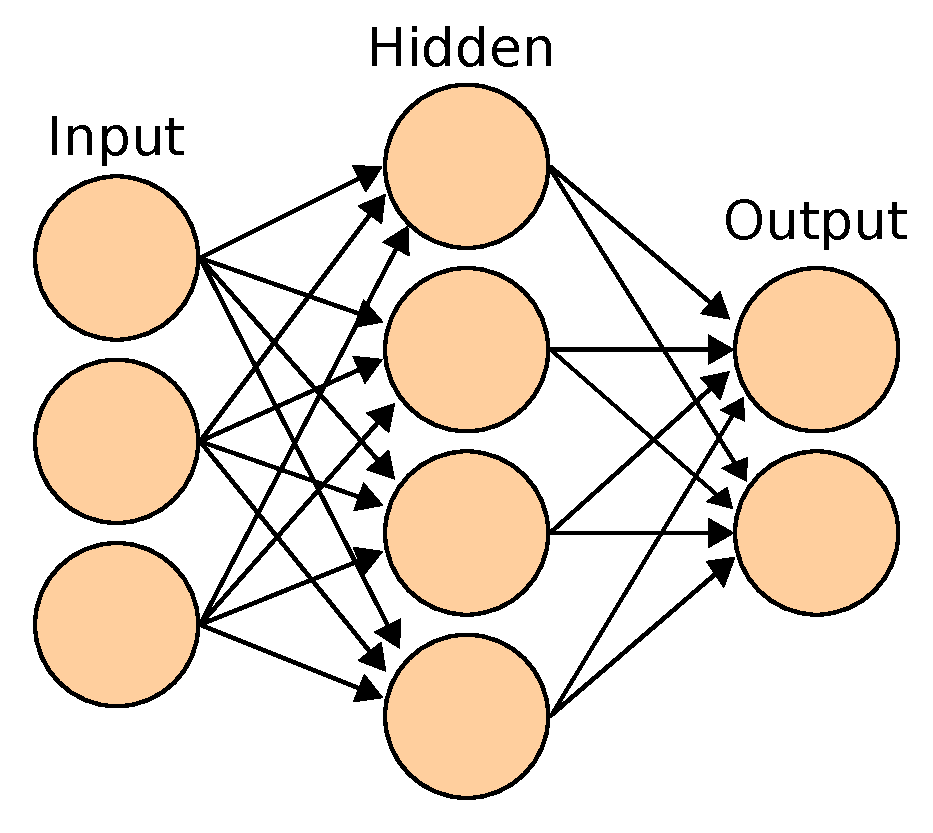
\includegraphics[width=0.5\textwidth]{figures/chapter2/ANN_diagram}
  \caption[Diagram of a simple ANN.]{Diagram of a simple ANN~\citep{ann-wiki-pic}.}
\label{fig:chap2-ann-layout}
\end{figure}

Each network has two special layers called the input and output layers. The input layer accepts information from which the ANN's designer wants data extracted. The output layer is responsible for producing the output which contains the information on how the network responded to the input excitation data. In-between these extreme layers lie the so-called `hidden' layers. These layers form the majority of the network and are responsible for interpreting the input data and producing the network's output. 

The connections between the hidden nodes are represented by a weighting factor which are determined during a training process. These weights define how much influence the nodes have over another, i.e.\ if a weight is positive, it excites another node, whereas if it is negative, it suppresses the node. The input information traverses the hidden layers, activating the next node with the highest connection weighting. The output data is then determined by which of the nodes were traversed in the hidden layers. The connections between the hidden node layers are mostly responsible for the output and different connection schemes provide different performance characteristics. 

Consider a simple example: you wish to create an ANN to recognise whether a picture contains a man or a dog. You train it with 25 images of different men and dogs, telling the ANN which picture contains which. After it has been trained, you show it a picture containing a young boy which is totally unfamiliar to the network. Based on the way you trained it, the network should recognise enough human and male features in the child to come to the conclusion that it is more likely that the child is a man rather than it is being a dog. 

This ability to classify information that technically falls out of the network's training environment is one of the strengths of ANNs. This advantage, as stated by~\cite{tu1996advantages}, is ANNs' ability to implicitly detect any non-linear relationships between multi-dimensional input and output dimensions. They can also be trained using different training schemes and some modern software packages and libraries have also made it fairly easy to develop a model without any formal statistical training. Some drawbacks of ANNs are that they may require an immense amount of computing power if many nodes are initialised, they are prone to overfitting data when a poorly selected number of nodes are used and the trained models are extremely `black-box' solutions, making it difficult to identify and characterise the relationships between the nodes. 

Different ANN topologies and layouts, have been developed and proposed. Some of them are briefly discussed in the following sections.

\subsubsection{Feed-forward Network}

The oldest, and arguably the simplest ANN topography is the feed-forward network (FFN), also referred to as multi-layer perceptron if there are multiple layers in the hidden layer. Its layout is typically similar to the one given in Figure~\ref{fig:chap2-ann-layout}, with a single input and output layer, as well as a single or multiple hidden node layers. 

The FFN uses some form of supervised training algorithm, with the backpropagation algorithm commonly used. Here, the hidden nodes' weights are adjusted until the output the network produces is as close as possible to the target output specified by the designer. This configuration's biggest attractions are its simplicity, relatively fast training speed, depending on the number of hidden layers, and its ability to derive non-linear relationships between dimensions. However, FFN's are prone to converging very slowly and sometimes getting stuck in local minima, as stated by~\cite{svozil1997introduction}. However, improvements to the backpropagation training scheme have reduced this effect.

\subsubsection{Recurrent Neural Network}

The recurrent neural network (RNN) is a family of neural networks. The hidden nodes of an RNN make provision for feedback between the different hidden layers and the output layer, creating an internal state for the network. See Figure~\ref{fig:chap2-rnn-diagram} for a diagram of a RNN topography.

\begin{figure}
 \centering
 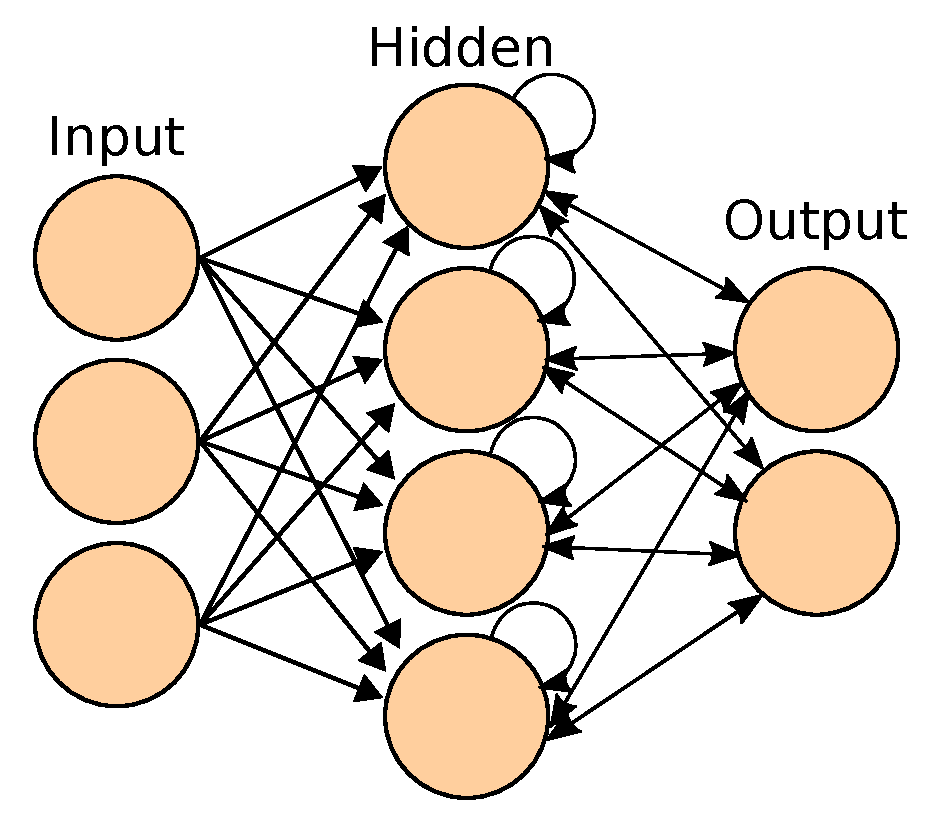
\includegraphics[width=0.5\textwidth]{figures/chapter2/rnn_diagram}
 \caption[Diagram of a simple RNN.]{A diagram of a simple RNN (adapted from~\citeauthor{ann-wiki-pic}, \citeyear{ann-wiki-pic}).}
\label{fig:chap2-rnn-diagram}
\end{figure}

In contrast to the FFN, this internal saved state allows the RNN to process arbitrary sequences of input data, making it adept at processing unsegmented speech or handwriting patterns. However, the added complexity of adding feedback loops between the different layers becomes computationally expensive, especially when large networks with many layers and inputs are used. Increases in computing power and improvements in the training process, as well as a better understanding of RNNs and ANNs in general, have alleviated the computational expense somewhat.

There are different RNN configurations available. These include the Hopfield network~\citep{hopfield1982neural}, the echo network~\citep{jaeger2001echo} and the recurrent multilayer perceptron network~\citep{tutschku1995recurrent}.

\subsubsection{Radial Basis Function Network}

The radial basis function neural network (RBFNN) is another type of neural network and is a sub-family of the RNN family, as stated by~\cite{wilamowski1996implementation}. 

The RBFNN topology is fixed to a three-layer architecture, with one input layer, one hidden layer and one output layer. The input layer provides the input. The hidden layer then remaps these inputs to make them linearly separable, where the output layer does the separation and outputs the data~\citep{xie2011comparison}.  

Despite belonging to the same family of ANN, there are a number of significant differences between the RBFNN and RNN.\@ Firstly, the three-layer RBFNNs are simpler than multi-layered RNNs, making the training process for RBFNNs generally faster than for an RNN.\@ Secondly, and most importantly, as stated by~\citeauthor{xie2011comparison}, is the difference in how the RBFNN and RNN classifies the data: the RBFNN data clusters are separated by a hyper sphere, whereas RNNs use arbitrarily shaped hyper surfaces. See Figure~\ref{fig:chap2-classifier} for a visualisation of these class separation strategies. This makes RBFNNs an attractive option to interpolate multidimensional data.

\begin{figure*}
  \centering
  \begin{subfigure}{0.5\textwidth}
    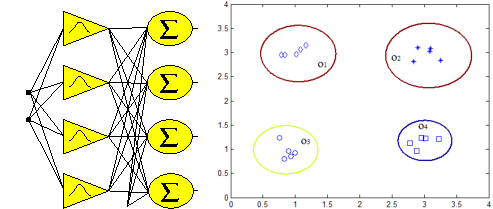
\includegraphics[width=\textwidth]{figures/chapter2/rbf_class}
    \caption{}
    \label{fig:chap2-rbf-classifier}
  \end{subfigure}
  \begin{subfigure}{0.5\textwidth}
    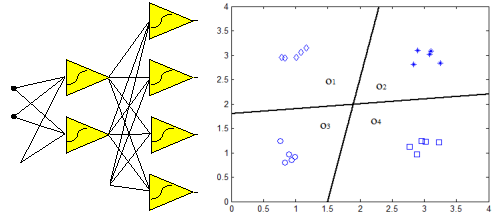
\includegraphics[width=\textwidth]{figures/chapter2/rnn_class}
    \caption{}
    \label{fig:chap2-rnn-classifier}
  \end{subfigure}
  \caption[Comparison between the RBF and RNN classifiers. ]{A comparison between the RBF classifier in Figure~\ref{fig:chap2-rbf-classifier} and the RNN classifier in Figure~\ref{fig:chap2-rnn-classifier} as shown by~\cite{xie2011comparison}. }
\label{fig:chap2-classifier}
\end{figure*}

\citeauthor{xie2011comparison} further determined that RBFNNs are well suited to interpolate noisy data where the data surfaces contain regular valleys and peaks. In contrast, normal ANNs and RNNs are more efficient for classification problems and for well-conditioned, regularly spaced data. 

As described by~\cite{skala2012radial}, the function on each node is given by 

\begin{equation}
  \label{eq:chap2-rbf}
  f(\bm{x}_i) = \sum\limits_{j = 1}^{M}\lambda_j \phi(|| \bm{x}_i - \bm{x}_j ||).
\end{equation}
Therein, $\lambda_j$ is the node weighting factor and $\bm{x}_j$ are the kernel centres which are determined during the model training phase. The function $\phi$ is the radial function of the euclidian norm of the distance between the node centre and the input vector. This radial function is variable and the designer can select the function which best describes the data, although a Gaussian radial function, i.e.\ $\phi(\bm{r}_{ij}) = e^{-(\frac{\bm{r}_{ij}}{\epsilon})^2}$, $\bm{r}_{ij} = || \bm{x}_i - \bm{x}_j ||$, is commonly used.  

\subsection{Support Vector Machines}

Support vector machines (SVM) is a widely used classification technique first proposed by~\cite{vapnik1995support}. It works by finding a hyperplane between two data classes that separates the classes by the widest possible average margin. See Figure~\ref{fig:chap2-svm-linear} for an illustration of this separation.

\begin{figure}
  \centering
  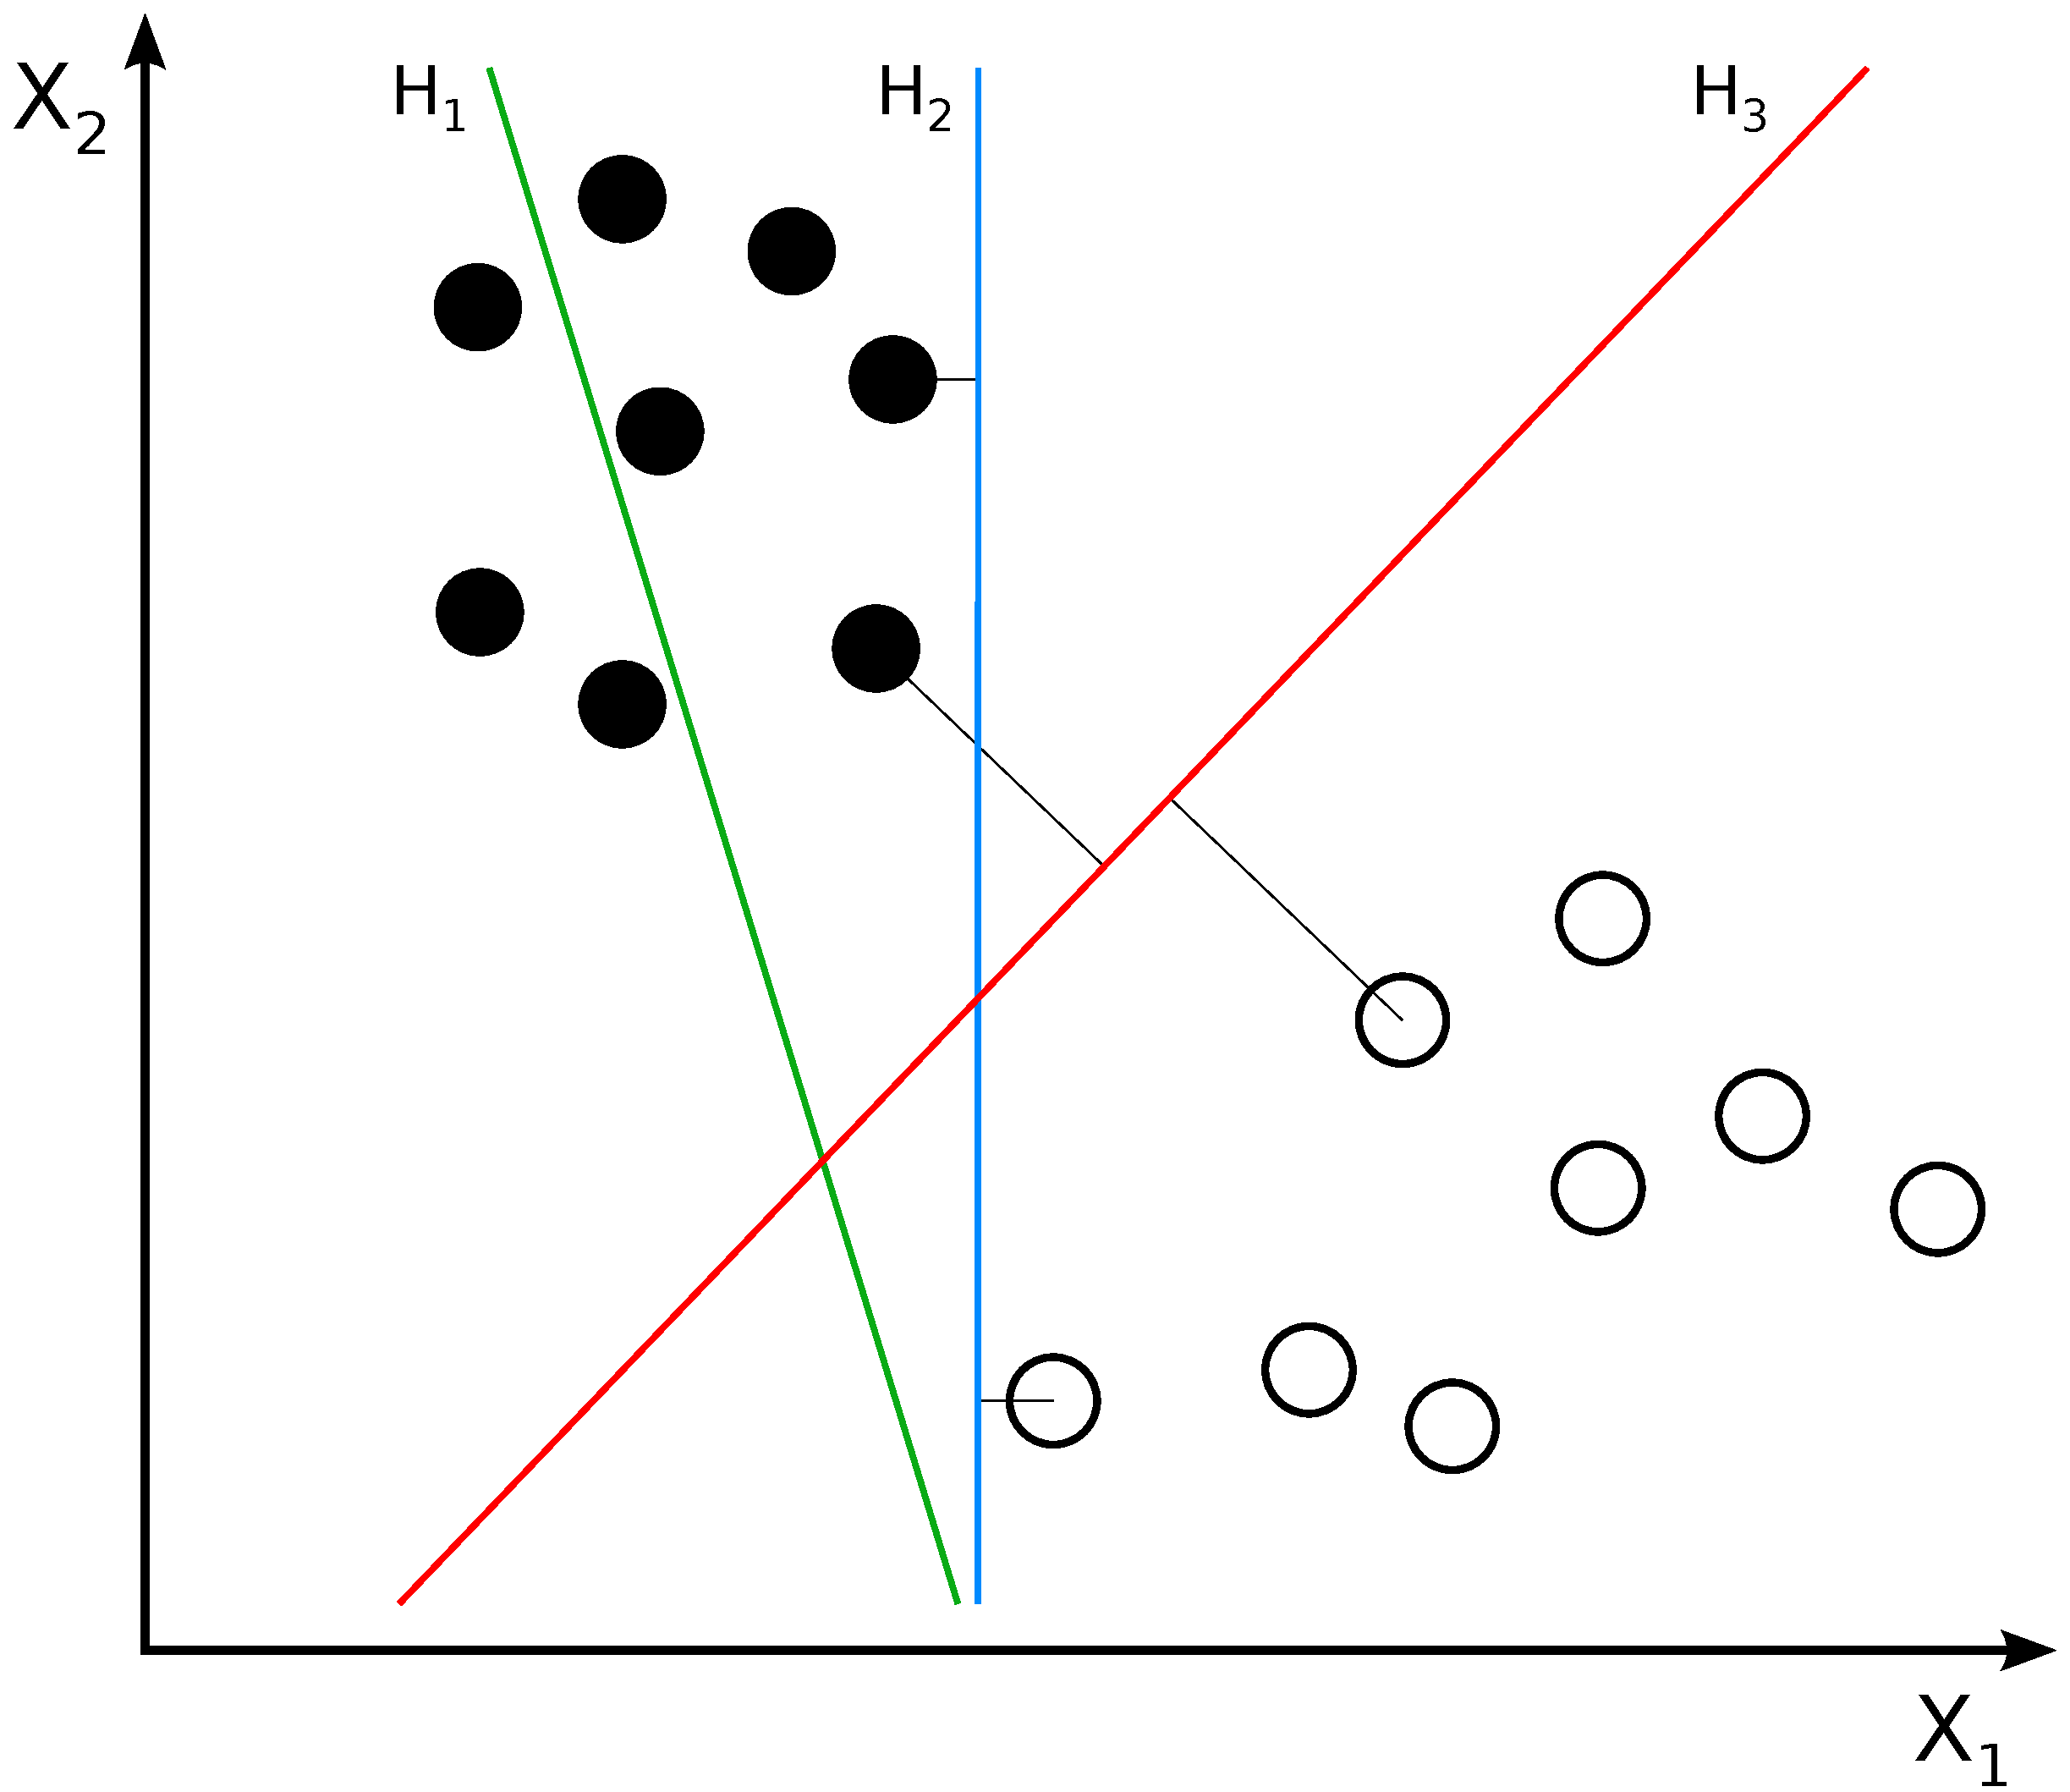
\includegraphics[width=0.5\textwidth]{figures/chapter2/svm_linear}
  \caption[SVM with a linear hyperplane.]{An SVM plot illustrating different class separators~\citep{svm-wiki-pic}.\@ $H_1$ does not separate the classes, while $H_2$ has only minimal class separation. $H_3$ exhibits the widest average separation margin.}
\label{fig:chap2-svm-linear}
\end{figure}

\citeauthor{vapnik1995support}'s original method was limited to linear hyperplanes. Since then, the algorithm has extended to non-linear hyperplanes by applying what is known as the `kernel trick', as described by~\cite{amari1999improving}. An example of such a non-linear separator can be seen in Figure~\ref{fig:chap2-svm-nonlinear}.

\begin{figure}
  \centering
  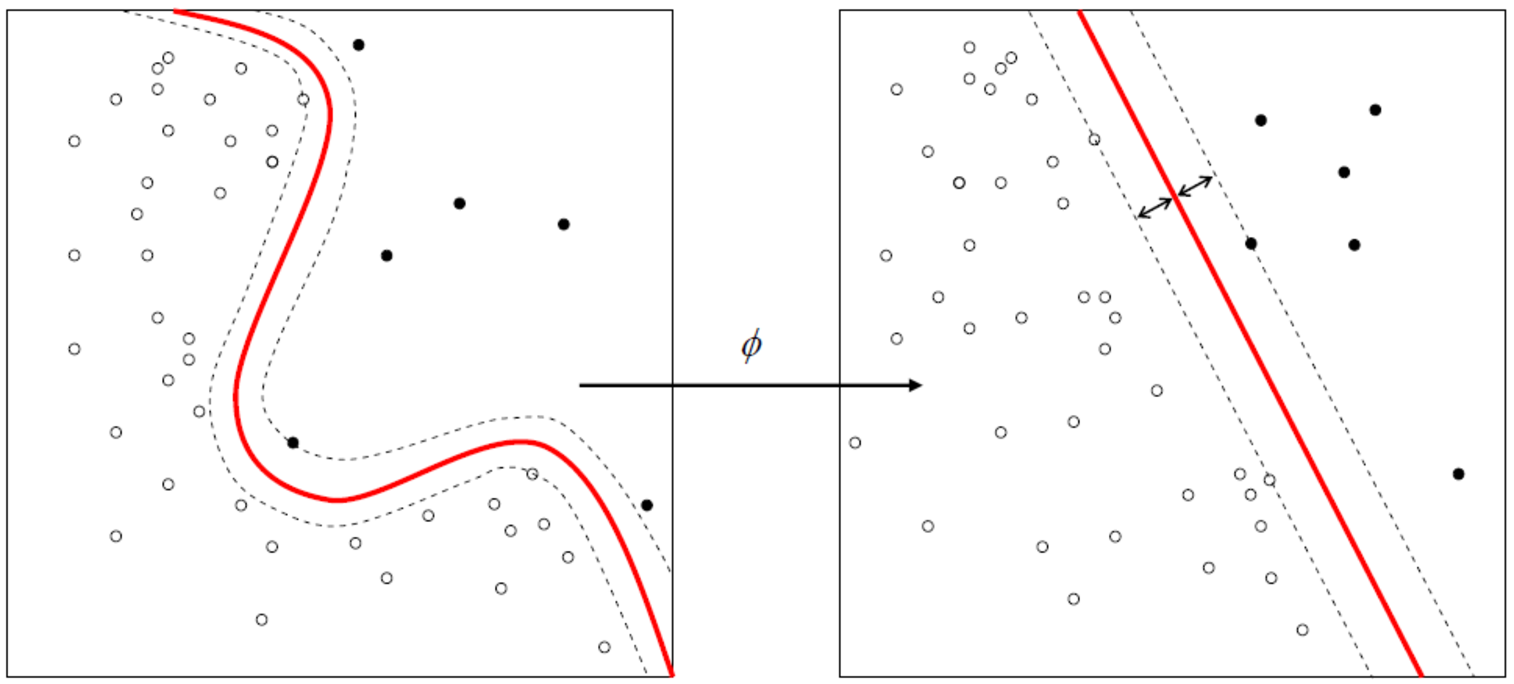
\includegraphics[width=0.8\textwidth]{figures/chapter2/svm_nonlinear}
  \caption[Example of an SVM with a non-linear kernel separator.]{An example of an SVM with a non-linear kernel separator~\citep{kernel-wiki-pic}.}
\label{fig:chap2-svm-nonlinear}
\end{figure}

SVM's are limited to  binary problems with two classes, somewhat limiting their potential for high-dimensional problems. Regardless, they are extremely popular in scientific circles due to their accuracy and relative simplicity. 

\section{Conclusion}

In this chapter, several concepts relevant to this project have been mentioned and discussed. Furthermore, past research findings, algorithms and techniques have also been identified. 

It was found that the stable control of a quadcopter in the outdoors is possible, thanks to improved mathematical models and sensors. It has also been established that a computer vision pose measurement system is feasible and there are freely availible libraries which are capable of it. Lastly, it was determined that artificial neural networks are well suited to this project's high dimensional nature. 

\chapter{Measurement System Design}
\label{chap3}

\section{Introduction}

The goal of this project is to determine the pose estimation accuracy of a quadcopter flying in the outdoors. In this context, the pose is a six-dimensional position and orientation vector given by $P = [R | \bm{T}]$, where the vector $\bm{T}$ contains the $[x\;y\;z]^T$ position dimensions and the matrix $R$ is an Eulerian rotation matrix. 

In order to determine the pose estimation accuracy of a quadcopter, two sets of data are required, the first being the quadcopter's own pose estimate and the second its true pose, as measured by an accurate external measurement tool. There are accurate measurement tools available for the outdoor environment, which include laser and sonar systems. However, they are fairly expensive systems and the necessary equipment was not available at the time this project was executed. It was therefore decided to investigate an alternative method of measuring a quadcopter's true pose in the outdoors.

A computer vision-based system was investigated and later implemented. Using a computer vision system (CVS) for measurement is an attractive option: it is simple, cheap, compact and easy to operate. However, the measurement accuracy of these systems differ between platforms. Therefore, a method of reliably determining a CVS's pose measurement accuracy must also be developed before the CVS can be used to make pose measurements of a quadcopter. 

This chapter sets out to provide detail on the design process of the CVS.\@ First, the design and layout of the CVS is discussed, then the method employed to determine the pose measurement accuracy is provided finally followed by the results of the entire process, from testing to data processing.

\section{Computer Vision System Layout}
\label{sec:chap3-cvs-layout}

\subsection{Introduction}

The CVS has both hardware and software components, both of which are important to making accurate pose measurements. In this section, the layout and design of the CVS, including its hardware and software components, is discussed, providing a broad overview of the system's make-up and how it functions. 

\subsection{System Overview and Requirements}

The CVS is to be used to make pose measurements of a quadcopter in flight. Its pose measurements must be accurate enough that it can be used as reference pose data when comparing it to a quadcopter's on-board pose data to determine the pose accuracy of a quadcopter. The CVS has to fulfil the following objectives:

\begin{itemize}
  \item The CVS must be able to make six-dimensional pose measurements.
  \item The CVS should provide measurements with an accuracy better than the quadcopter's on-board estimate.
  \item The CVS should make reliable, consistent pose measurements.
\end{itemize}

To meet these requirements, a CVS was designed and implemented. The proposed computer vision measurement system makes use of the following processes and procedures: 

\begin{itemize}
  \item Camera parameter estimation and calibration.
  \item Automated two-dimensional image feature detection.
  \item Pose data extraction and derivation.
  \item Data noise reduction. 
\end{itemize}

\subsection{Software}
\label{sec:cv-sys-software}

The CVS is a system which extracts information of interest from an arbitrary image. There is a strong software aspect to the CVS, since it relies on well-researched and understood computer vision techniques and algorithms. To this end, the popular open source OpenCV library\footnote{OpenCV v2.4.8} was used to perform the computer vision tasks. This library was used since its free, readily available, has a wide support network on the internet and comes pre-packaged with a large variety of up-to-date and powerful computer vision functions. To perform the numerical matrix operations, the open source NumPy\footnote{NumPy v1.8.2} library for the Python\footnote{Python v2.7} language was used. 

OpenCV was used to calibrate the CVS's camera, extract feature data from a video stream and determine the pose of a calibration pattern by solving the principle n-points (PnP) problem. The entire process is described here. 

First, the camera is calibrated by following the procedure discussed in Chapter~\ref{chap2}. Here, a $5\times6$ square chessboard pattern was used for calibration. To summarise the procedure, the OpenCV functions \emph{findChessboardCorners()} and \emph{findCornersSubPix()} are used to detect and extract two-dimensional coordinate data of the corners on the chessboard pattern from a still image. These coordinates, along with their three-dimensional world coordinates, are fed to the \emph{calibrateCamera()} function to produce the camera matrix. The calibration procedure produces the camera matrix $C$, as presented in Equation~\ref{eq:chap2-cam-matrix} and repeated here again in Equation~\ref{eq:chap3-cam-matrix} for the reader's convenience. 

\begin{equation}
  \label{eq:chap3-cam-matrix}
  C = 
  NP
\end{equation}

In Equation~\ref{eq:chap3-cam-matrix}, the matrix $N$ is given by Equation~\ref{eq:chap3-cam-intrinsic} and matrix $P$ by Equation~\ref{eq:chap3-cam-extrinsic}.

\begin{equation}
  \label{eq:chap3-cam-intrinsic}
  N = 
  \begin{bmatrix}
    f_x & 0   & u_0 \\
    0   & f_y & v_0 \\
    0   & 0   & 1   \\
  \end{bmatrix}
\end{equation}

\begin{equation}
  \label{eq:chap3-cam-extrinsic}
  P = 
  \begin{bmatrix}
    R | \bm{T}
  \end{bmatrix}
  =
  \begin{bmatrix}
    r_{11} & r_{21} & r_{31} & t_1 \\
    r_{21} & r_{22} & r_{32} & t_2 \\
    r_{31} & r_{23} & r_{33} & t_3 \\
  \end{bmatrix}
\end{equation}

With the calibrated camera matrix $C$, it is now possible to use OpenCV's PnP problem solver to extract the camera's pose data. This procedure is based on the relation given in Equation~\ref{eq:chap3-2d-to-3d}, which relates the three-dimensional world coordinate vector $\bm{X}_w$, to its two-dimensional image projection $\bm{x}_c$.  

\begin{equation}
   \label{eq:chap3-2d-to-3d}
   \bm{x}_c
   = C
   \bm{X}_w
\end{equation}

Using the relation in Equation~\ref{eq:chap3-2d-to-3d} and the camera matrix $C$'s intrinsic parameters, OpenCV's \emph{solvePnPRansac()} function can be employed to extract the pose matrix $P$ of the camera relative to the calibration board. The PnP solver used is the robust PnP solver, employing Leverberg-Marquart optimsisation, as described by~\cite{schweighofer2006robust}. It was found that a $5\times6$ chessboard does not have enough corners features to guarantee accurate results from the ePnP method of~\cite{lepetit2009epnp}.

\subsection{Hardware}

The hardware requirements for the CVS are fairly minimal and its setup equally simple. To allow the software to make six-dimensional pose estimations, the hardware needs to capture image data at an appropriate resolution for OpenCV to be able to detect and extract the two-dimensional feature coordinate data. The camera should preferably not have a lens zoom function to keep the focal length constant throughout a measurement session. A computer running the OpenCV and data-processing scripts, as well as a calibration board, are also required. 

The camera that was used is a single Microsoft LifeCamHD webcam capable of capturing 720p high definition video data at a frame rate of 30 frames per second. This camera has a variable zoom feature, however, which was controlled and set to a constant value by using the \emph{uvcdynctrl} webcam control library\footnote{uvcdynctrl v0.2.4}. A stereo camera setup can also be used, however the accuracy between the single and stereo camera in most respects is rather negligible, except in the depth dimension where the stereo vastly outperforms the single camera. Much like a person with one eye closed, single cameras are notoriously bad at estimating depth, so bad depth estimates for this system is expected. For this implementation, the single camera variant was used, making the system simpler to set up and use, but care must be taken with the depth estimate. In the future, the project can be expanded to a stereo camera system if it is found that the inaccurate depth estimate significantly affects the measurement accuracy.

The calibration board used was a flat, ISO A1-sized\footnote{$\SI{841}{\mm}\times\SI{594}{\mm}$}, $5\times6$-square chessboard pattern calibration board. A large board was selected to allow the squares on it to be large, affording the camera a good view of the corners and improving the data extraction performance. The large board size also allowed for a fairly wide white border around the squares, as per OpenCV's recommendation. 

A laptop running Linux Mint 17.1 `Rebecca' was used as a ground control station for the quadcopter in subsequent measurement tests. In addition, it was used as a recording device along with the webcam and performed some of the data processing tasks, though a more powerful desktop PC was used to perform the image processing tasks. 

\section{Measurement Test Design}

\subsection{Introduction}

Before the CVS could be used to measure the pose of a quadcopter in flight, the accuracy of the CVS's measurements was first determined. The PnP solving algorithm is, at its core, an optimisation problem and only produces pose estimates. In light of this, determining the accuracy of the CVS's pose measurements, or estimates, is an important step in the system's design phase. 

To determine the measurement accuracy of the CVS, a measurement test was performed in an indoor environment where another external measurement device whose accuracy is high enough that its pose measurements can be taken as ground-truth values, could record pose data. The CVS's measurement error could then be determined by comparing the CVS's measurements with that of the external measurement system's. Both systems were set to record the pose of a flat chessboard pattern that was moved and orientated by hand.

This section describes the test layout, including the external measurement device and its details, as well as the CVS's details for the test. Then, the measurement procedure is presented, followed by the steps taken to process the data during the post-processing phase. 

\subsection{Test Layout}
\label{sec:vicon-test-setup}

\subsubsection{External Measurement Device Layout}

The external measurement system used to record the ground-truth pose data is a Vicon indoor motion capture system. It is a widely-used commercial system with applications in the film, medical and sporting industries and can reach sub-millimetre accuracy in its measurements, as found by~\cite{windolf2008systematic}. It works by tracking a set of infrared markers stuck to a surface with at least two infrared cameras and sophisticated proprietary motion tracking software and it does this at a rate of 300Hz. The Vicon only measures the position vector. Therefore, to get a complete pose vector including the orientation, trigonometric relationships between the different translation vectors were used to determine the angular orientation. Given its well-documented measurement accuracy, the measurement results from this system was taken as ground-truth.

The Vicon system used for the test is located in the 3D Human Motion Laboratory on Stellenbosch University's Tygerberg medical campus. It consists of eight infrared cameras arranged around a square on the floor in a configuration that maximises the number of infrared markers visible to each camera at any given point in time. Figure~\ref{fig:chap3-vicon-layout} shows a diagram of the Vicon system layout. 
 
\begin{figure}
  \centering
  \def\svgwidth{0.5\textwidth}
  \input{figures/chapter3/vicon_layout.pdf_tex}
  \caption[Layout of the Vicon motion capture system.]{Layout of the Vicon motion capture system. Note that this is not drawn to scale.}
\label{fig:chap3-vicon-layout}
\end{figure}

Before the measurement test commenced, the Vicon system was calibrated using a calibration procedure similar to the CVS's, but the calibration object used is a special calibration `wand' whose dimensions are pre-programmed into the Vicon system. Then, infrared markers were placed on both the calibration board and the CVS's camera to provide pose data on both. Since the Vicon and CVS camera each have their own coordinate systems, having the position and orientation of the CVS's camera available will allow the Vicon's measurements to be related back to the CVS's camera coordinate system during the data processing phase. The markers were placed in such a way that they produce axes that more or less coincide with the Vicon's axis system, slightly simplifying the data processing phase. Figure~\ref{fig:chap3-cam-vicon-axes} shows the axis systems for both the CVS and Vicon systems.

\begin{figure}
  \centering
  \def\svgwidth{0.5\textwidth}
  \input{figures/chapter3/cam_vicon_axis.pdf_tex}
  \caption{The axis orientations of the Vicon and CV systems.}
\label{fig:chap3-cam-vicon-axes}
\end{figure}

Only three markers need to be visible to the Vicon system's cameras for it to record an object's position vector, which can then be used to produce a six-dimensional pose vector. However, a fourth asymmetrical auxiliary marker was also placed to provide fail-safe orientation data during the data processing phase. Figures~\ref{fig:chap3-cam-marker-placement} and~\ref{fig:chap3-board-marker-placement} show the marker placements for the camera and the calibration board. These markers were carefully placed by hand in line with one another, but some placement error is inevitable. This placement error offset is taken into account during the data processing phase. 

\begin{figure}
   \centering 
   \includegraphics[clip, trim = 0 400 0 400, width=0.6\textwidth]{figures/chapter3/cam_1.pdf}
   \caption{Infrared marker placement on the camera.}
\label{fig:chap3-cam-marker-placement}
\end{figure}

\begin{figure}
   \centering 
   \includegraphics[clip, trim = 600 0 400 0, width=0.6\textwidth]{figures/chapter3/bord_2.pdf}
   \caption{Infrared marker placement on the chessboard.}
\label{fig:chap3-board-marker-placement}
\end{figure}

One aspect of the Vicon system to note is that the infrared markers have some high-frequency noise associated with them, which is apparent when inspecting the raw data. This noise is inherent to the marker and can be safely filtered out with a zero-lag, second order Butterworth filter. However, to avoid any unknown filtering factors from the Vicon system from affecting the data, the raw, unfiltered data is used throughout this project. 

\subsubsection{Computer Vision System Setup}

The CVS configuration used during the Vicon test is the exact same as the one described in Section~\ref{sec:chap3-cvs-layout}.

Before the test, the CVS's camera was calibrated to determine its intrinsic parameters, including its focal lengths in the $x$ and $y$ directions. Calibration was done with the same board and camera that was used during the Vicon test, against a white, well-lit background. The board was moved to different positions and orientations within view of the camera, and roughly 15 still images at a resolution of $640\times480$ pixels were taken. The camera was then calibrated with this set of images and OpenCV's camera calibration module to produce a camera matrix that gives a reprojection error of approximately 0.21 pixel units. It was found that capturing data at a higher resolution did not produce significantly better results and slowed the feature data extraction process down. The focal length was found to be approximately 700 pixel units in both the $x$ and $y$ directions.

In the test, the camera was placed in a stable, aluminium frame and was left untouched throughout the test. The laptop was set to only capture video at $640\times480$ pixels, while zoom and autofocus was disabled to keep the camera's lens focal length constant. The data extraction and pose estimation took place off-line. 

\subsection{Test Procedure}

Figure~\ref{fig:chap3-pic-sys-layout} shows a picture of the complete test setup. As described in Section~\ref{sec:vicon-test-setup}, the camera is placed on a chair and the calibration board is held facing the camera. Both are covered with four infrared markers, with the eight infrared cameras of the Vicon system surrounding both the board and camera.  

\begin{figure}
  \centering
  \includegraphics[clip, trim = 600 300 0 0, width=0.7\textwidth]{figures/chapter3/sys_1.pdf}
  \caption{Picture of the test layout.}
\label{fig:chap3-pic-sys-layout}
\end{figure}

Data capture for both systems started when the Vicon system started recording data. At the same time, the chessboard was tilted forward, allowing both measurement data sets to be synchronised to a common timeframe during the data processing phase. 

During the data capturing phase, it was desirable to record a variety of pose vector combinations. This was done by moving the calibration board around the CVS camera's full field of vision and depth of view, while simultaneously varying the board's rotation angles, producing a diverse data cloud in both the CVS's and Vicon system's data sets. 

Each video is approximately 90 seconds long, equating to approximately 2700 pose vector samples per test, though it was decided that only 2400 of these points will be used to compensate for any invalid or inconsistent readings. 

The measurement test produced two sets of measurement data: one ground-truth pose measurement data set from the Vicon system and one measurement data set from the CVS\@. These data sets allows for the determination of the CVS's measurement error by comparing the two sets of measurement data. These sets were also used to provide training and validation data sets for the error prediction model discussed in Chapter~\ref{chap4}. 

\subsection{Data Processing}

\subsubsection{Introduction}

During the measurement test, the CVS only captured video data, leaving the feature data extraction and pose estimation to be done off-line during the data processing phase. 

The Vicon system's data requires little processing, since most of the data is generated in real-time and is optimised by the Vicon software. However, some work was done to fix invalid measurements that were introduced when not enough Vicon cameras had a good view of the infrared markers for a few frames. These points were corrected by means of interpolation.

Processing the CVS data involved several steps, the first of which was to make the data sets directly relatable by centering both data sets around a common axis system. Furthermore, the marker placement and other error offsets were determined while optimising the camera matrix's focal lengths to produce the most accurate CVS pose measurement results. Each of these aspects are discussed next.

\subsubsection{Reducing Vicon Sample Speed}

The Vicon system captures data at 300Hz and the CVS at 30Hz. Therefore, the Vicon's framerate had to be downsampled to match the CVS's framerate so that the two data sets could directly be related. 

The process involved averaging the Vicon data set in intervals of 10 samples, downsampling the Vicon by a factor of 10 and matching the CVS's framerate. This approach was taken to ensure that no data that might contain valuable information and trends gets discarded. 

\subsubsection{Rotating and Centring the Camera and Chessboard Data}
\label{sec:rotate-axes}

During the measurement test, four infrared markers were placed on the CVS camera's frame to provide data on its placement within the Vicon's axis system. The markers were placed along the frame's $x$ and $y$ axes and coincided with the chessboard's axis system. Since the CVS's camera remained still during the test, it is most convenient to centre the CVS's camera and pose measurement data around the Vicon's axis system. 

With the CVS's camera placement and orientation in the Vicon coordinate system known, relocating and reorientating the CVS's camera pose data became a relatively simple task. Since the CVS's position and orientation remained constant throughout the measurement test, its data could be centred around the Vicon axis system by simply subtracting the CVS's placement coordinates from each of the measurement vectors produced by the CVS.

With the CVS's camera axis system now centred around the Vicon system's origin, the pose data for the chessboard acquired by the CVS and the Vicon system are now directly relatable to one another.  

\subsubsection{Camera Parameter Optimisation}
\label{sec:focal-optimisation}

Before the measurement test took place, the CVS camera was calibrated using OpenCV's camera calibration toolbox. The calibration procedure provides a good estimate of the intrinsic parameters of the camera, which includes the focal lengths. However, given the lack of reference three-dimensional data, it is only an estimate of the intrinsic parameters. Using the ground-truth pose data from the Vicon system will allow the intrinsic parameters to be determined more accurately. Since the Vicon's infrared markers were not placed exactly on the calibration board's $x$ and $y$ axes, the infrared marker placement offset error must also be taken into account and determined. This offset error will account for the marker placement error, as well as any other constant measurement bias that may have been introduced into the CVS's measurements. 

This presents a circular optimisation problem: the focal length will affect the perceived error offset, while the error offset will affect the CVS pose estimates, which in turn affects the ideal focal length. To find the offset and optimum focal length, a dual optimisation strategy was implemented.  

First, the optimisation algorithm is formulated. Suppose $\bm{P}^*$ denotes the six-dimensional pose vector of the calibration board (before it is centred around the Vicon's axis system) as produced by the Vicon system, while $\bar{\bm{P}}$ is the constant error offset vector and the subscripts $c$ and $b$ represent the data sets of the camera and calibration board respectively. $\bm{\epsilon}$ refers to the error vector between the Vicon and CVS's measurements that needs to be determined and $\bm{P}(f)$ is the pose vector measured by the CVS's camera as a function of its focal lengths $f_x$ and $f_y$. The Vicon pose and offset vectors are given by Equations~\ref{eq:chap3-calibration-pose} and~\ref{eq:chap3-offset}.

\begin{equation}
 \label{eq:chap3-calibration-pose}
  \bm{P}^* = \bm{P}^*_b - \bm{P}^*_c
\end{equation}

\begin{equation}
  \label{eq:chap3-offset}
  \bar{\bm{P}} = \bar{\bm{P}}_b - \bar{\bm{P}}_c
\end{equation}

The equation for the pose estimate from the CVS is given in Equation~\ref{eq:chap3-cvs}.

\begin{equation}
  \label{eq:chap3-cvs}
  \bm{P}(f) = \bm{P}^* - \bar{\bm{P}} + \bm{\epsilon}
\end{equation}

Equation~\ref{eq:chap3-cvs} can be simplified to the form given in Equation~\ref{eq:chap3-pose}, which forms the basis of the optimisation algorithm moving forward.  

\begin{equation}
  \label{eq:chap3-pose}
  \bm{P}(f_x, f_y) = (\bm{P}^*_b - \bar{\bm{P}}_b) - (\bm{P}^*_c - \bar{\bm{P}}_c) + \bm{\epsilon}
\end{equation}

The next step is then to determine the constant perceived offset for a given focal length combination. The focal length is initialised with the focal lengths found during calibration (approximately 700 pixel units in both directions). The offset can then determined using Equation~\ref{eq:chap3-eq1-offset}.

\begin{equation}
  \label{eq:chap3-eq1-offset}
  \sum\limits_i \bm{P}_i(f) - \sum\limits_i(\bm{P}^*_{b,i} - \bm{P}^*_{c, i}) = i\bar{\bm{P}} + \sum\limits_i\bm{\epsilon}_i
\end{equation}

At this point, it is assumed that the error vector $\bm{\epsilon}$ is normally distributed around zero, eliminating its sum and leading to Equation~\ref{eq:chap3-eq2-offset}. This assumption will be verified in Section~\ref{sec:err-norm-test}. 

\begin{equation}
  \label{eq:chap3-eq2-offset}
  i\bar{\bm{P}} = \sum\limits_i \bm{P}_i(f) - \sum\limits_i(\bm{P}^*_{b,i} - \bm{P}^*_{c, i})
\end{equation}

Using the constant $\bar{\bm{P}}$ produced by Equation~\ref{eq:chap3-eq2-offset}, it is now possible to minimise the error $\bm{\epsilon}$ from Equation~\ref{eq:chap3-pose} by varying the focal lengths $f_x$ and $f_y$. The minimum focal lengths were found by setting up a $3\times n$ error matrix, consisting of the three translation dimensions, ${[x\;y\;z]}^T$, where $n$ is the number of samples in the data set, and find the optimal focal length combination by minimising the vector's two-norm. The optimisation is based only on these three dimensions since it was found that including the orientation dimensions added too much variability to the procedure, leading to instability. The error matrix is produced by Equation~\ref{eq:chap3-error-base}.

\begin{equation}
  \label{eq:chap3-error-base}
  \bm{\epsilon} = \bm{P}(f) - \bm{P}^* - \bar{\bm{P}}
\end{equation}

Using the $3\times n$ error matrix from Equation~\ref{eq:chap3-error-base}, an error vector is generated by summing the error matrix along its columns. The optimum focal lengths were then found by taking the focal length combination that produces the smallest two-norm of the sample error vector $\bm{\epsilon}$. The minimisation equation is given by Equation~\ref{eq:chap3-err-min}.

\begin{equation}
  \label{eq:chap3-err-min}
  \min_{f_x, f_y}\left \Vert \sum_i  \bm{\epsilon}_i \right \Vert
\end{equation}

With the optimal focal length now determined, the procedure is repeated again from Equation~\ref{eq:chap3-pose}, finding a new offset for the new focal length combination. The optimisation procedure is iterated a number of times, minimising the total error norm. After the optimum focal length combination was found, that combination was used in the camera matrix that extracted the pose data from the video data.

In summation, the algorithm goes as follows: 

\begin{enumerate}
  \item Initialise focal lengths with values from the calibration procedure. 
  \item Repeat $k$ times:
  \begin{enumerate}
    \item Find $\bar{\bm{P}}$ for a constant $f_x$ and $f_y$ (Equation~\ref{eq:chap3-eq2-offset}).
    \item Determine the error vector $\bm{\epsilon}$ with a new $\bar{\bm{P}}$ (Equation~\ref{eq:chap3-error-base}).
    \item Update focal lengths $f_x$ and $f_y$ with the focal length combination that minimises $\left \Vert \bm{\epsilon} \right \Vert$ (Equation~\ref{eq:chap3-err-min}).
  \end{enumerate}
  \item Use the new focal lengths to estimate the chessboard's pose.
\end{enumerate}

\section{Results}

\subsection{Introduction}

Several sets of data were produced during the data processing phase. The results are presented and discussed in this section. They include evidence of error convergence for the optimisation procedure, as well as proofs that the error $\bm{\epsilon}$ is indeed normally distributed around zero. Lastly, the new focal length combination is given and discussed, followed by the pose measurement accuracy results of the CVS. 

\subsection{Evidence of Convergence}

BESPREEK FOUTE OOR HERSIEN MEME

To show that the optimisation procedure worked as expected, minimising the error in each pose dimension, the error after each iteration of the procedure is plotted. These plots are given in Figure~\ref{fig:err-convergence} and shows the errors over 50 iterations of optimisation.  

\begin{figure*}
  \centering
  \begin{subfigure}{0.45\textwidth}
    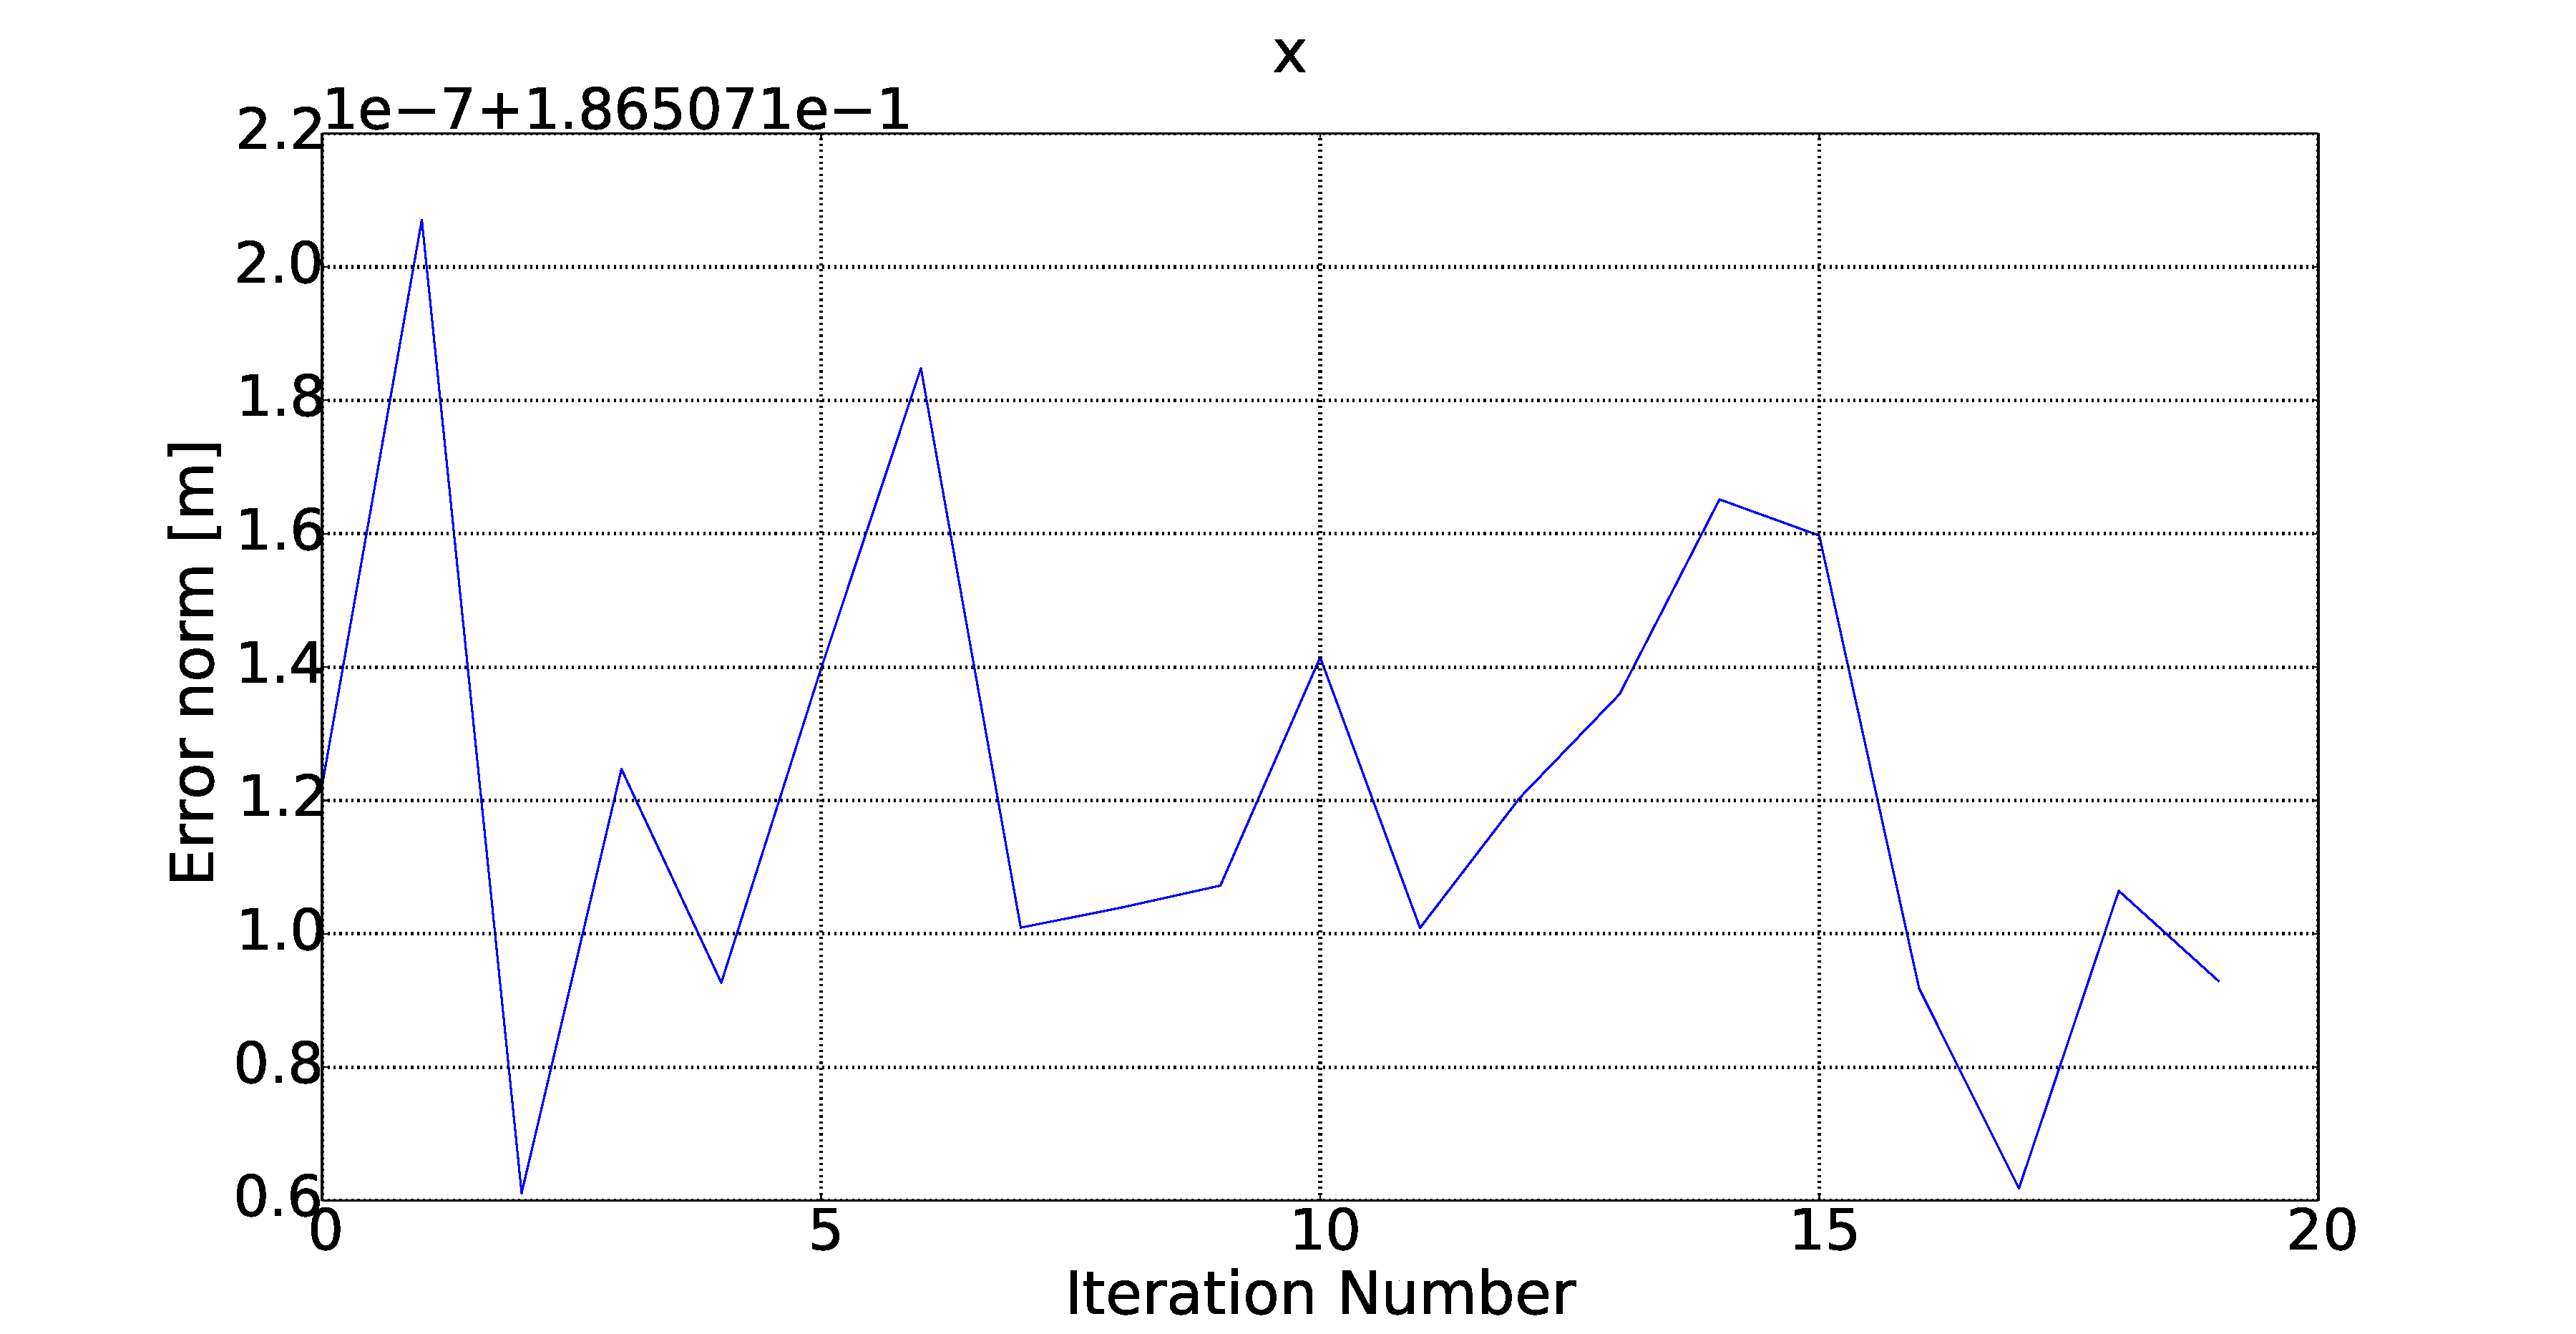
\includegraphics[width=\textwidth]{figures/chapter3/err_x.pdf}
    \caption{Error convergence in the $x$ dimension [m].}
\label{fig:err-convergence-x}
  \end{subfigure}
~
  \begin{subfigure}{0.45\textwidth}
    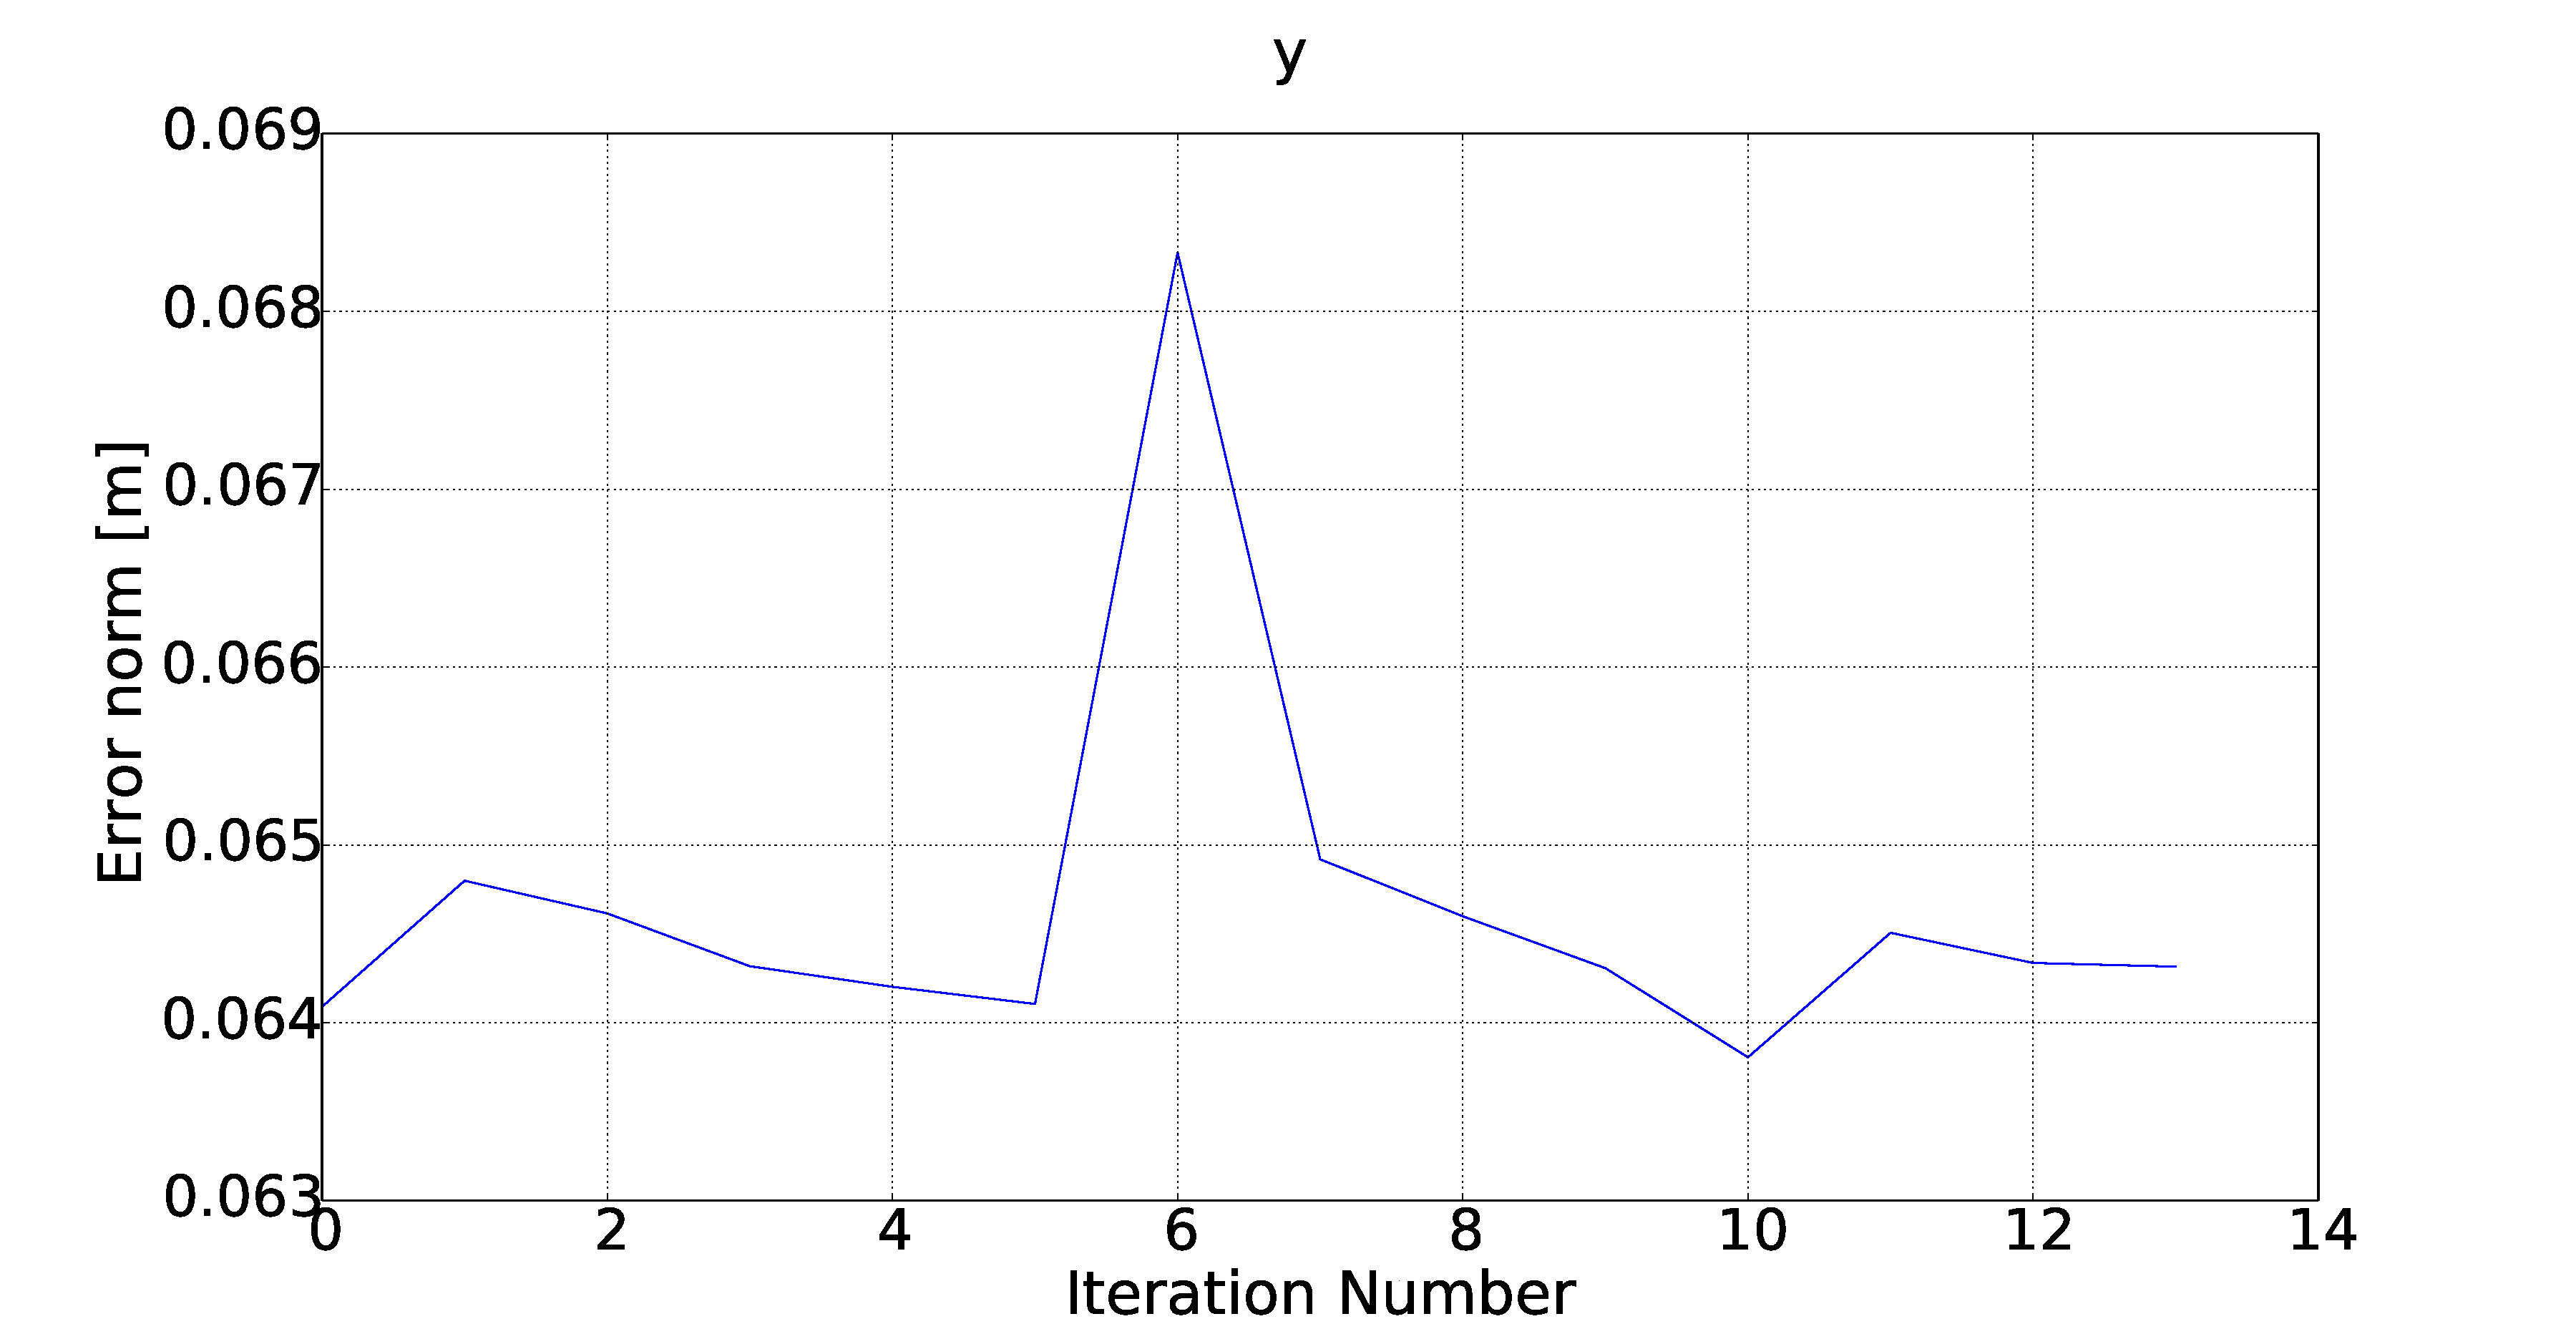
\includegraphics[width=\textwidth]{figures/chapter3/err_y.pdf}
    \caption{Error convergence in the $y$ dimension [m].}
\label{fig:err-convergence-y}
  \end{subfigure}
~
\begin{subfigure}{0.45\textwidth}
    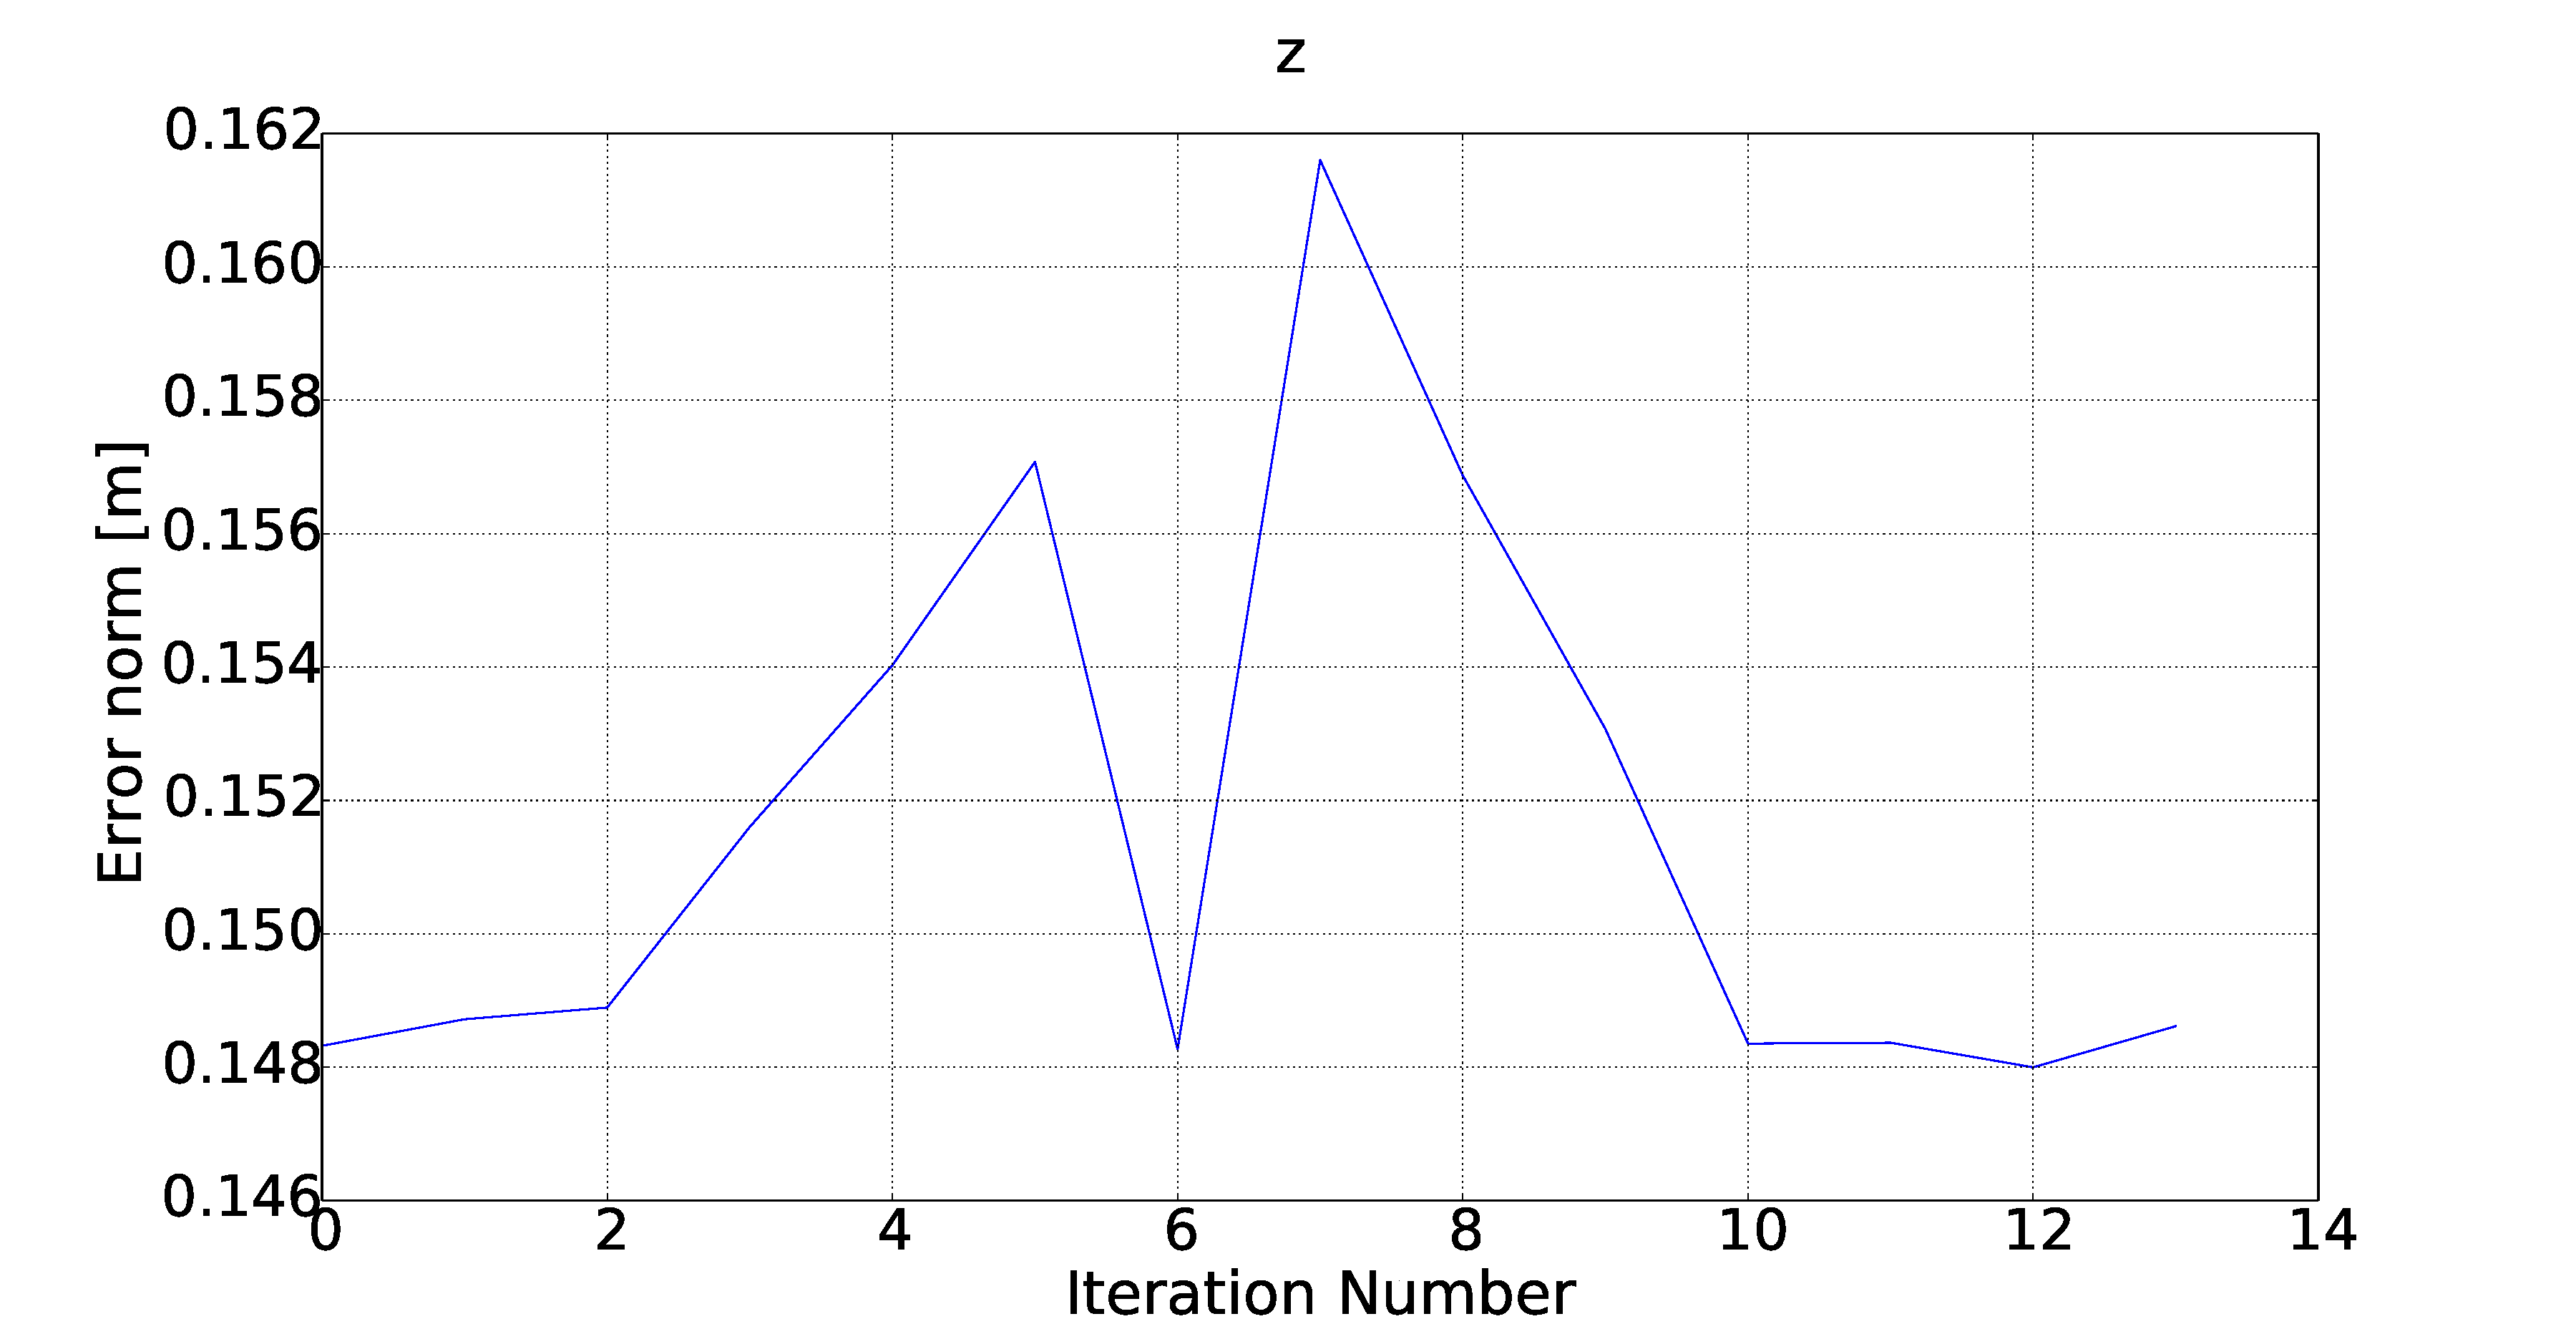
\includegraphics[width=\textwidth]{figures/chapter3/err_z.pdf}
    \caption{Error convergence in the $z$ dimension [m].}
\label{fig:err-convergence-z}
  \end{subfigure}
~
  \begin{subfigure}{0.45\textwidth}
    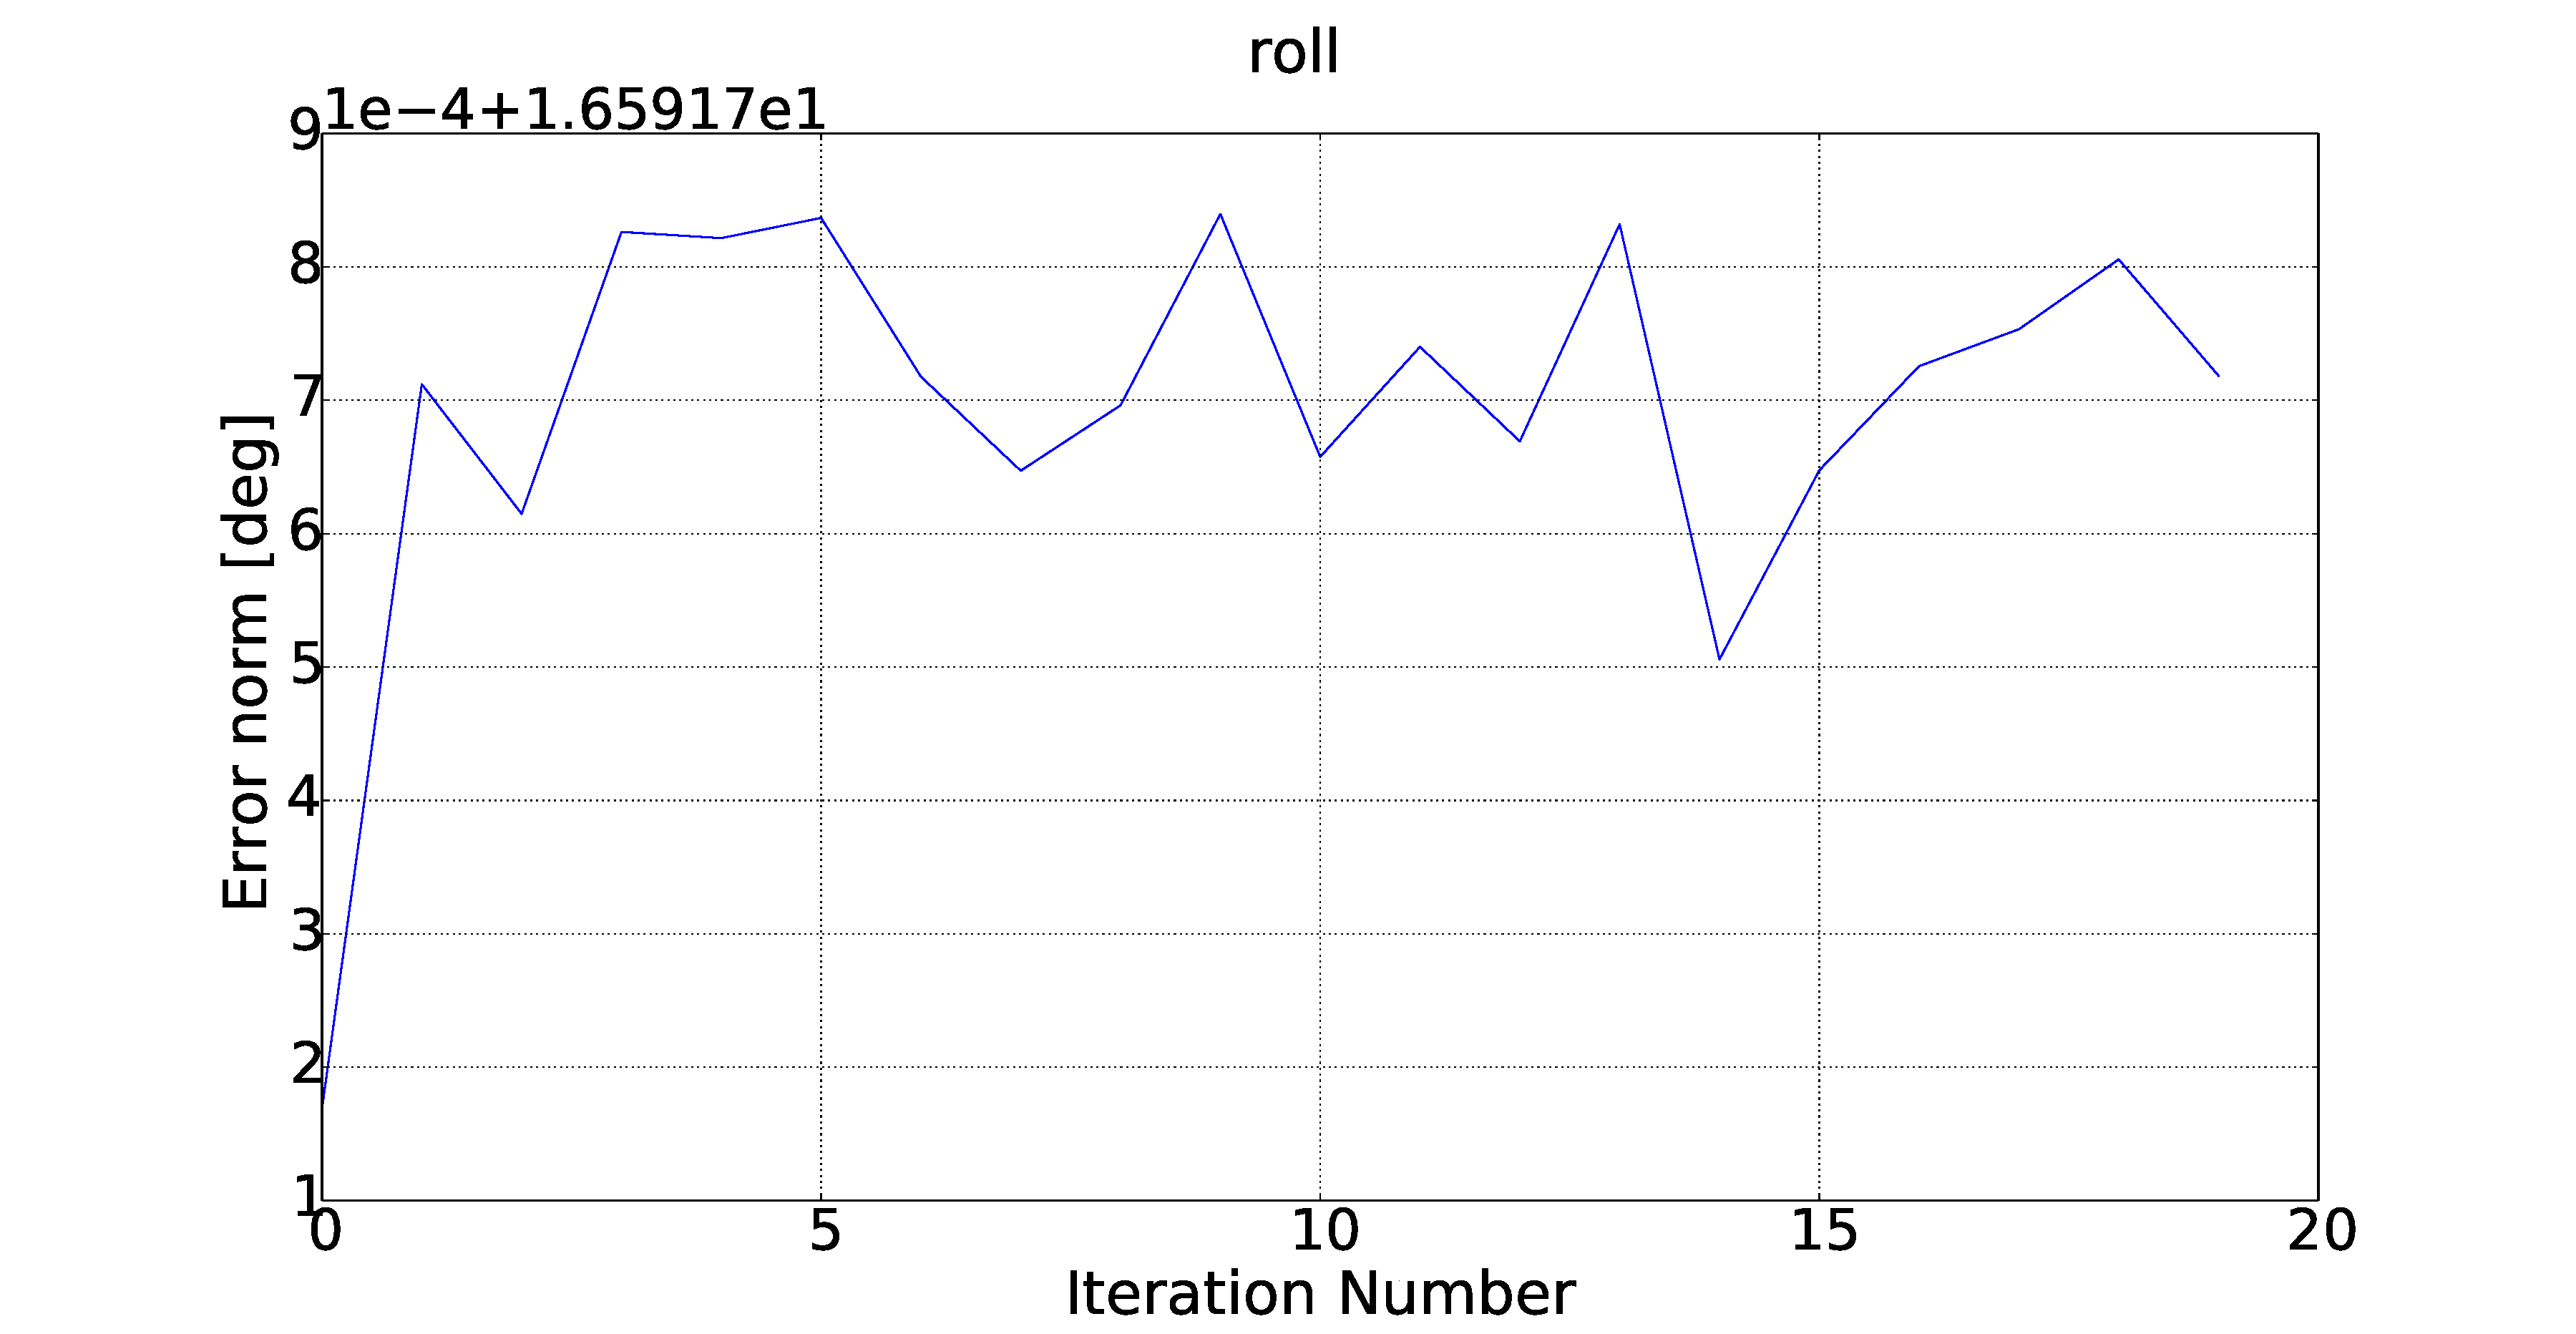
\includegraphics[width=\textwidth]{figures/chapter3/err_roll.pdf}
    \caption{Error convergence in the $\theta$ dimension [degrees].}
\label{fig:err-convergence-roll}
  \end{subfigure}
~
  \begin{subfigure}{0.45\textwidth}
    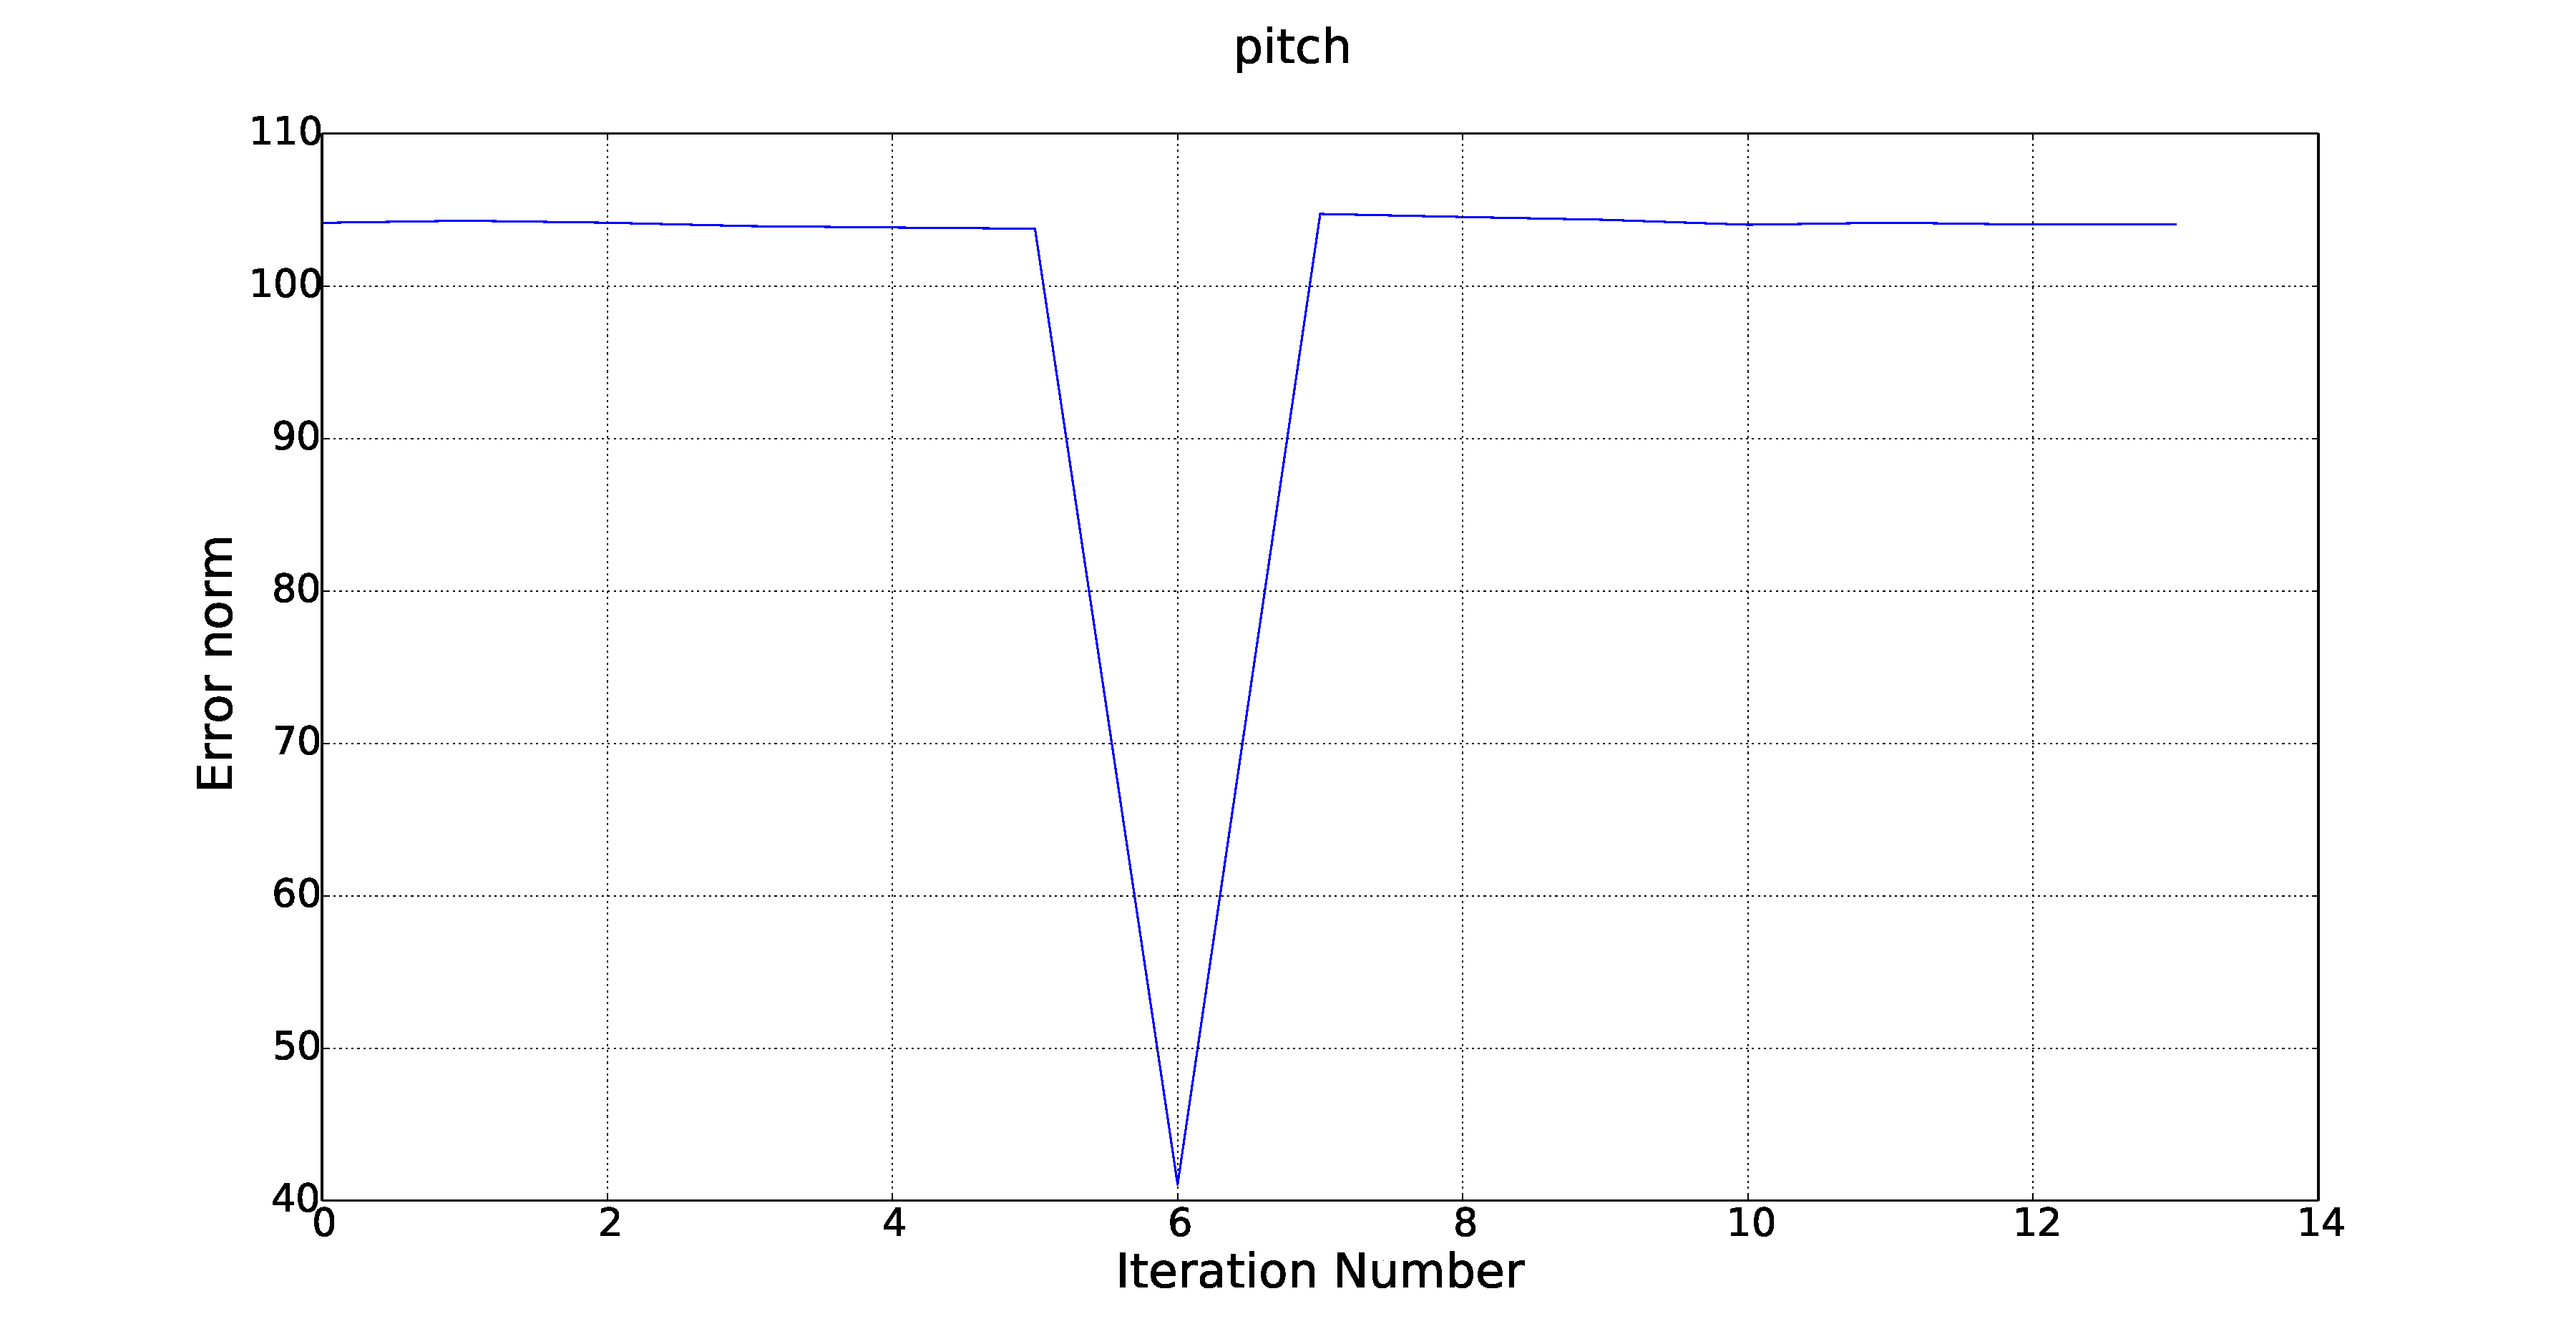
\includegraphics[width=\textwidth]{figures/chapter3/err_pitch.pdf}
    \caption{Error convergence in the $\phi$ dimension [degrees].}
\label{fig:err-convergence-pitch}
  \end{subfigure}
~
  \begin{subfigure}{0.45\textwidth}
    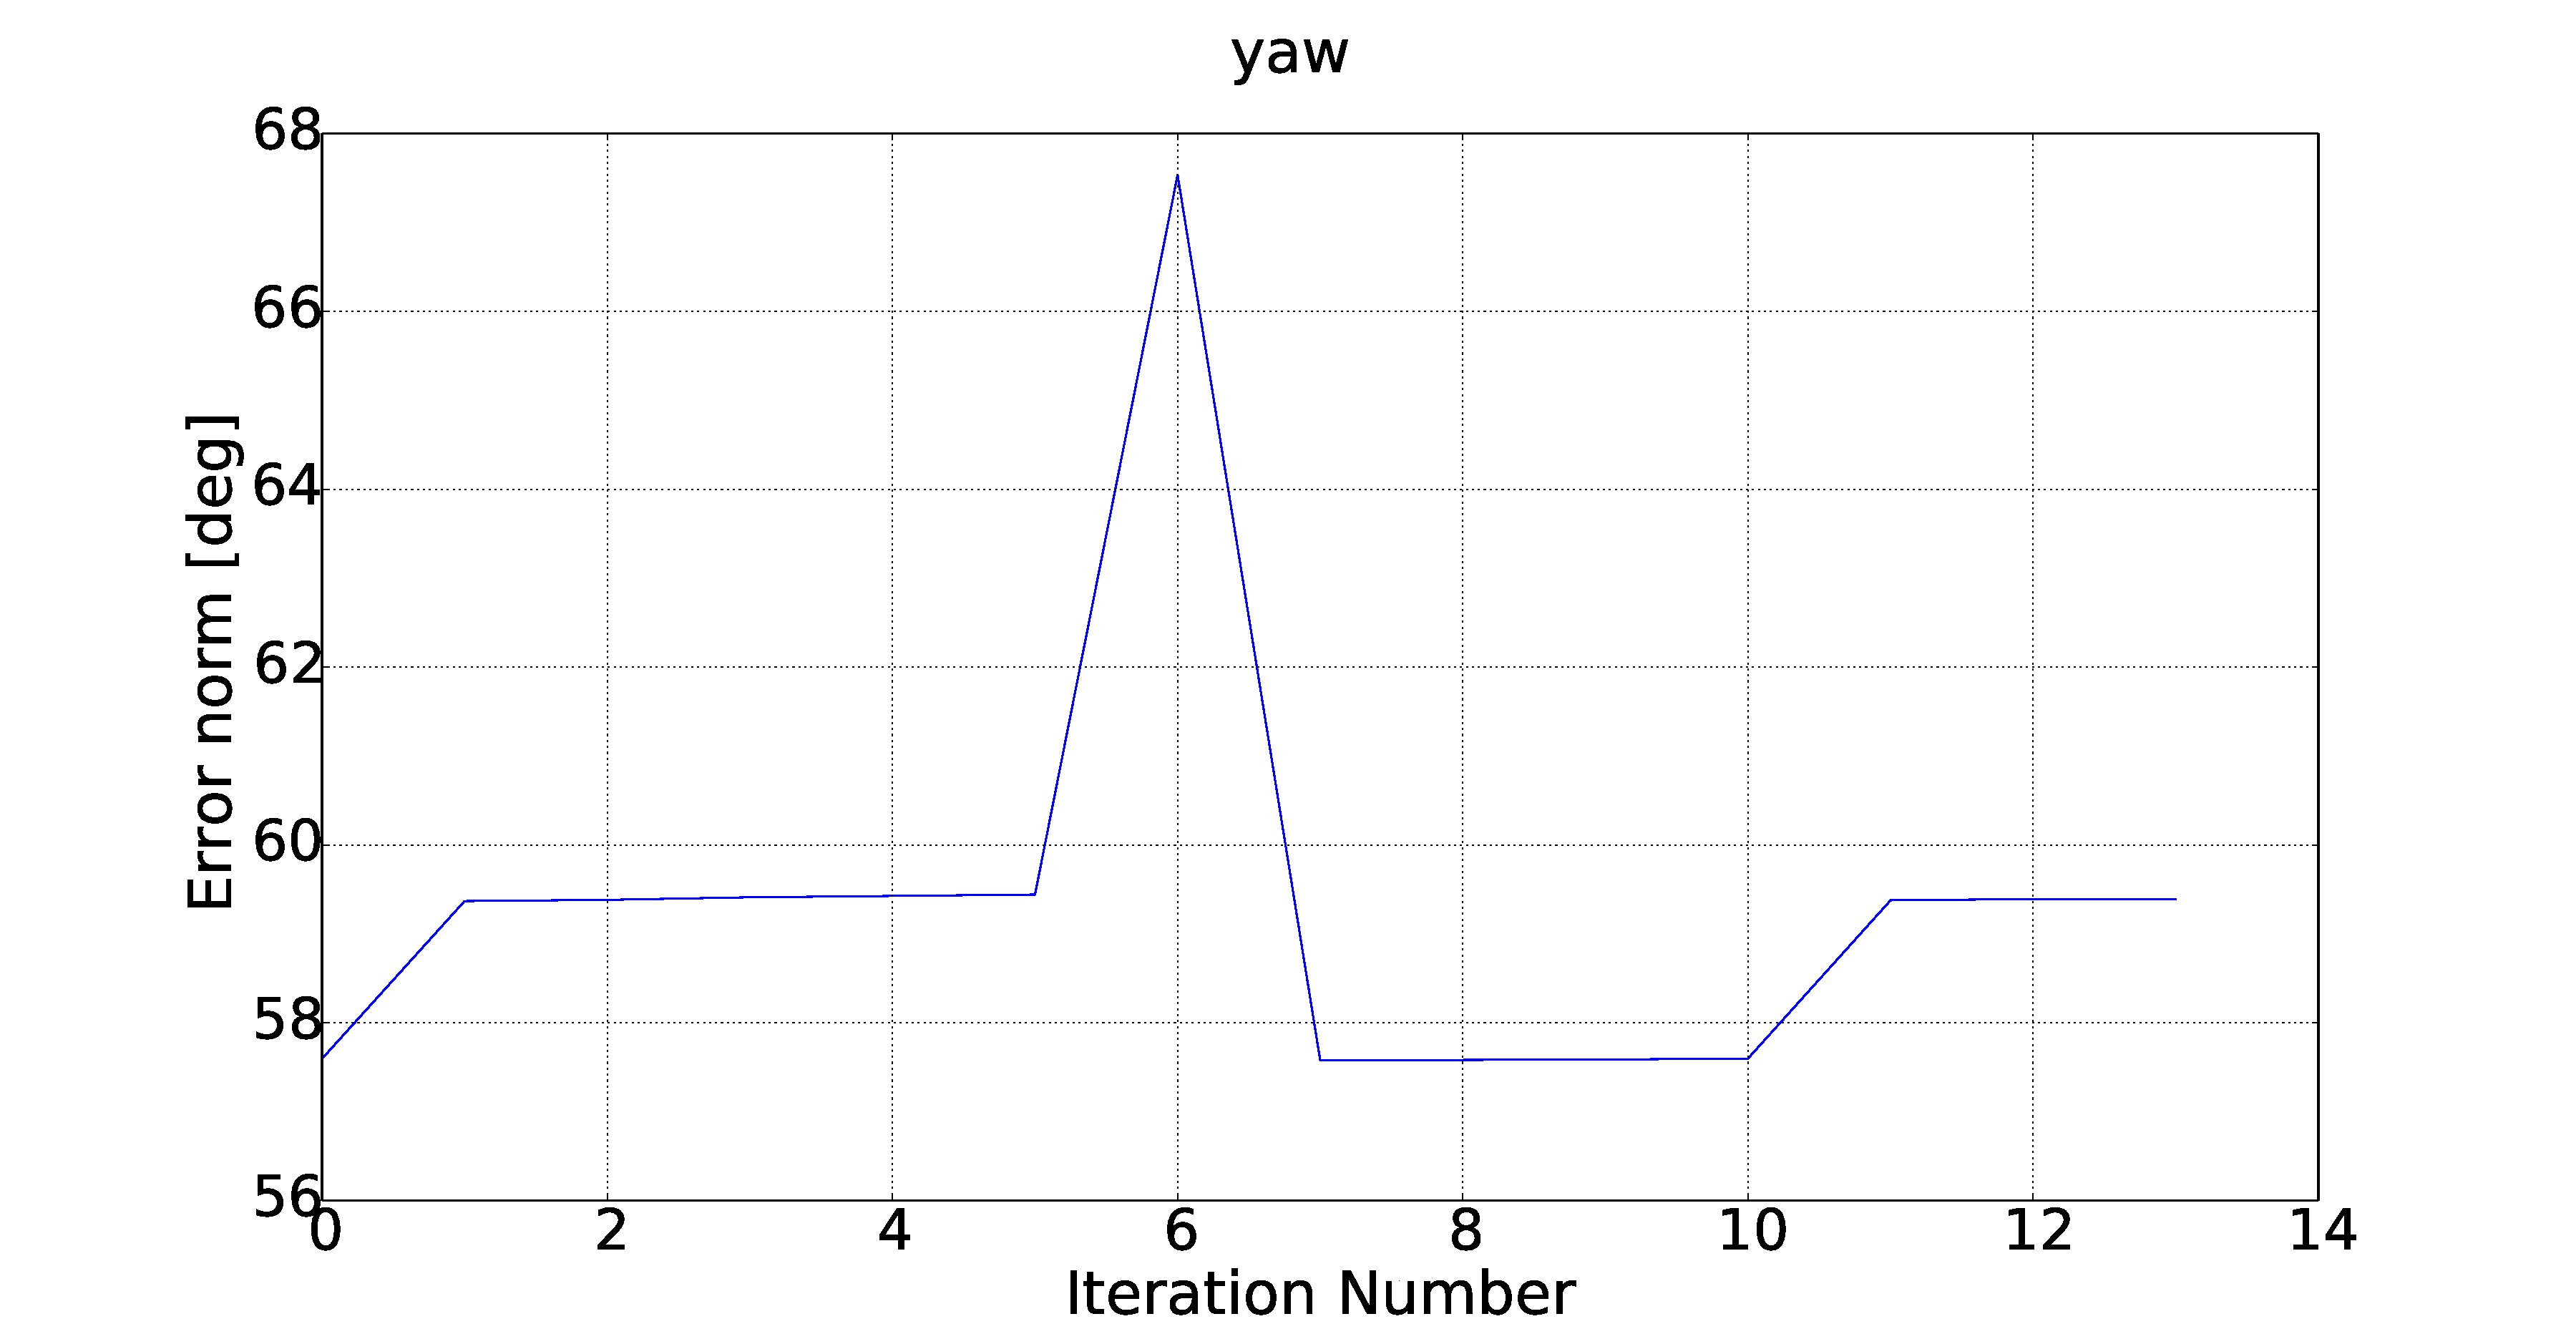
\includegraphics[width=\textwidth]{figures/chapter3/err_yaw.pdf}
    \caption{Error convergence in the $\psi$ dimension [degrees].}
\label{fig:err-convergence-psi}
  \end{subfigure}
  \caption[Plots showing error convergence for the optimsation procedure.]{Plots showing the error in each dimension during for each iteration of the error minimisation procedure.}
  \label{fig:err-convergence}
\end{figure*}

The graphs in Figure~\ref{fig:err-convergence} show that the error gets reduced in the $x$ and $z$ dimensions, while it gets worse in the $y$ and all of the orientation angle dimensions. 

The errors in the orientation angle dimensions are growing, since they carry no weight in the optimisation cost function. As for the growing error in the $y$ dimension, closer inspection of the graph shows that the $y$ dimension initially has the smallest error. It may be argued that since all three translation dimensions carry equal weight in the optimisation cost function, the $x$ and $z$ dimensions are being reduced at the cost of the error in the $y$ dimension. 

\subsection{Test for Normality}
\label{sec:err-norm-test}

HERSIEN DIE PLOTTE EN ALS MEME

To check if the error in $\bm{\epsilon}$ is indeed normally distributed, as assumed in Equation~\ref{eq:chap3-eq2-offset}, frequency histograms of the error matrix $\bm{\epsilon}$ in all six dimensions are plotted along with a normal distribution drawn using each dimension's mean and standard deviation. A $\chi^2$ (chi-squared) test could also have been used. However, it was found that the sample size of the data set was too large and it is known that some skewness in the data can have a large impact on the $\chi^2$ probability estimate CITE???. Therefore, a graphical approach was taken to determining if the errors are normally distributed around zero. 

Figure~\ref{fig:err-norm} shows the frequency histogram plots of the CVS measurement errors in the six dimensions. A normal distribution, using the averages and standard deviations from the data set, are superimposed to illustrate the normal distribution of the data.

\begin{figure*}
  \begin{subfigure}{0.48\textwidth}
    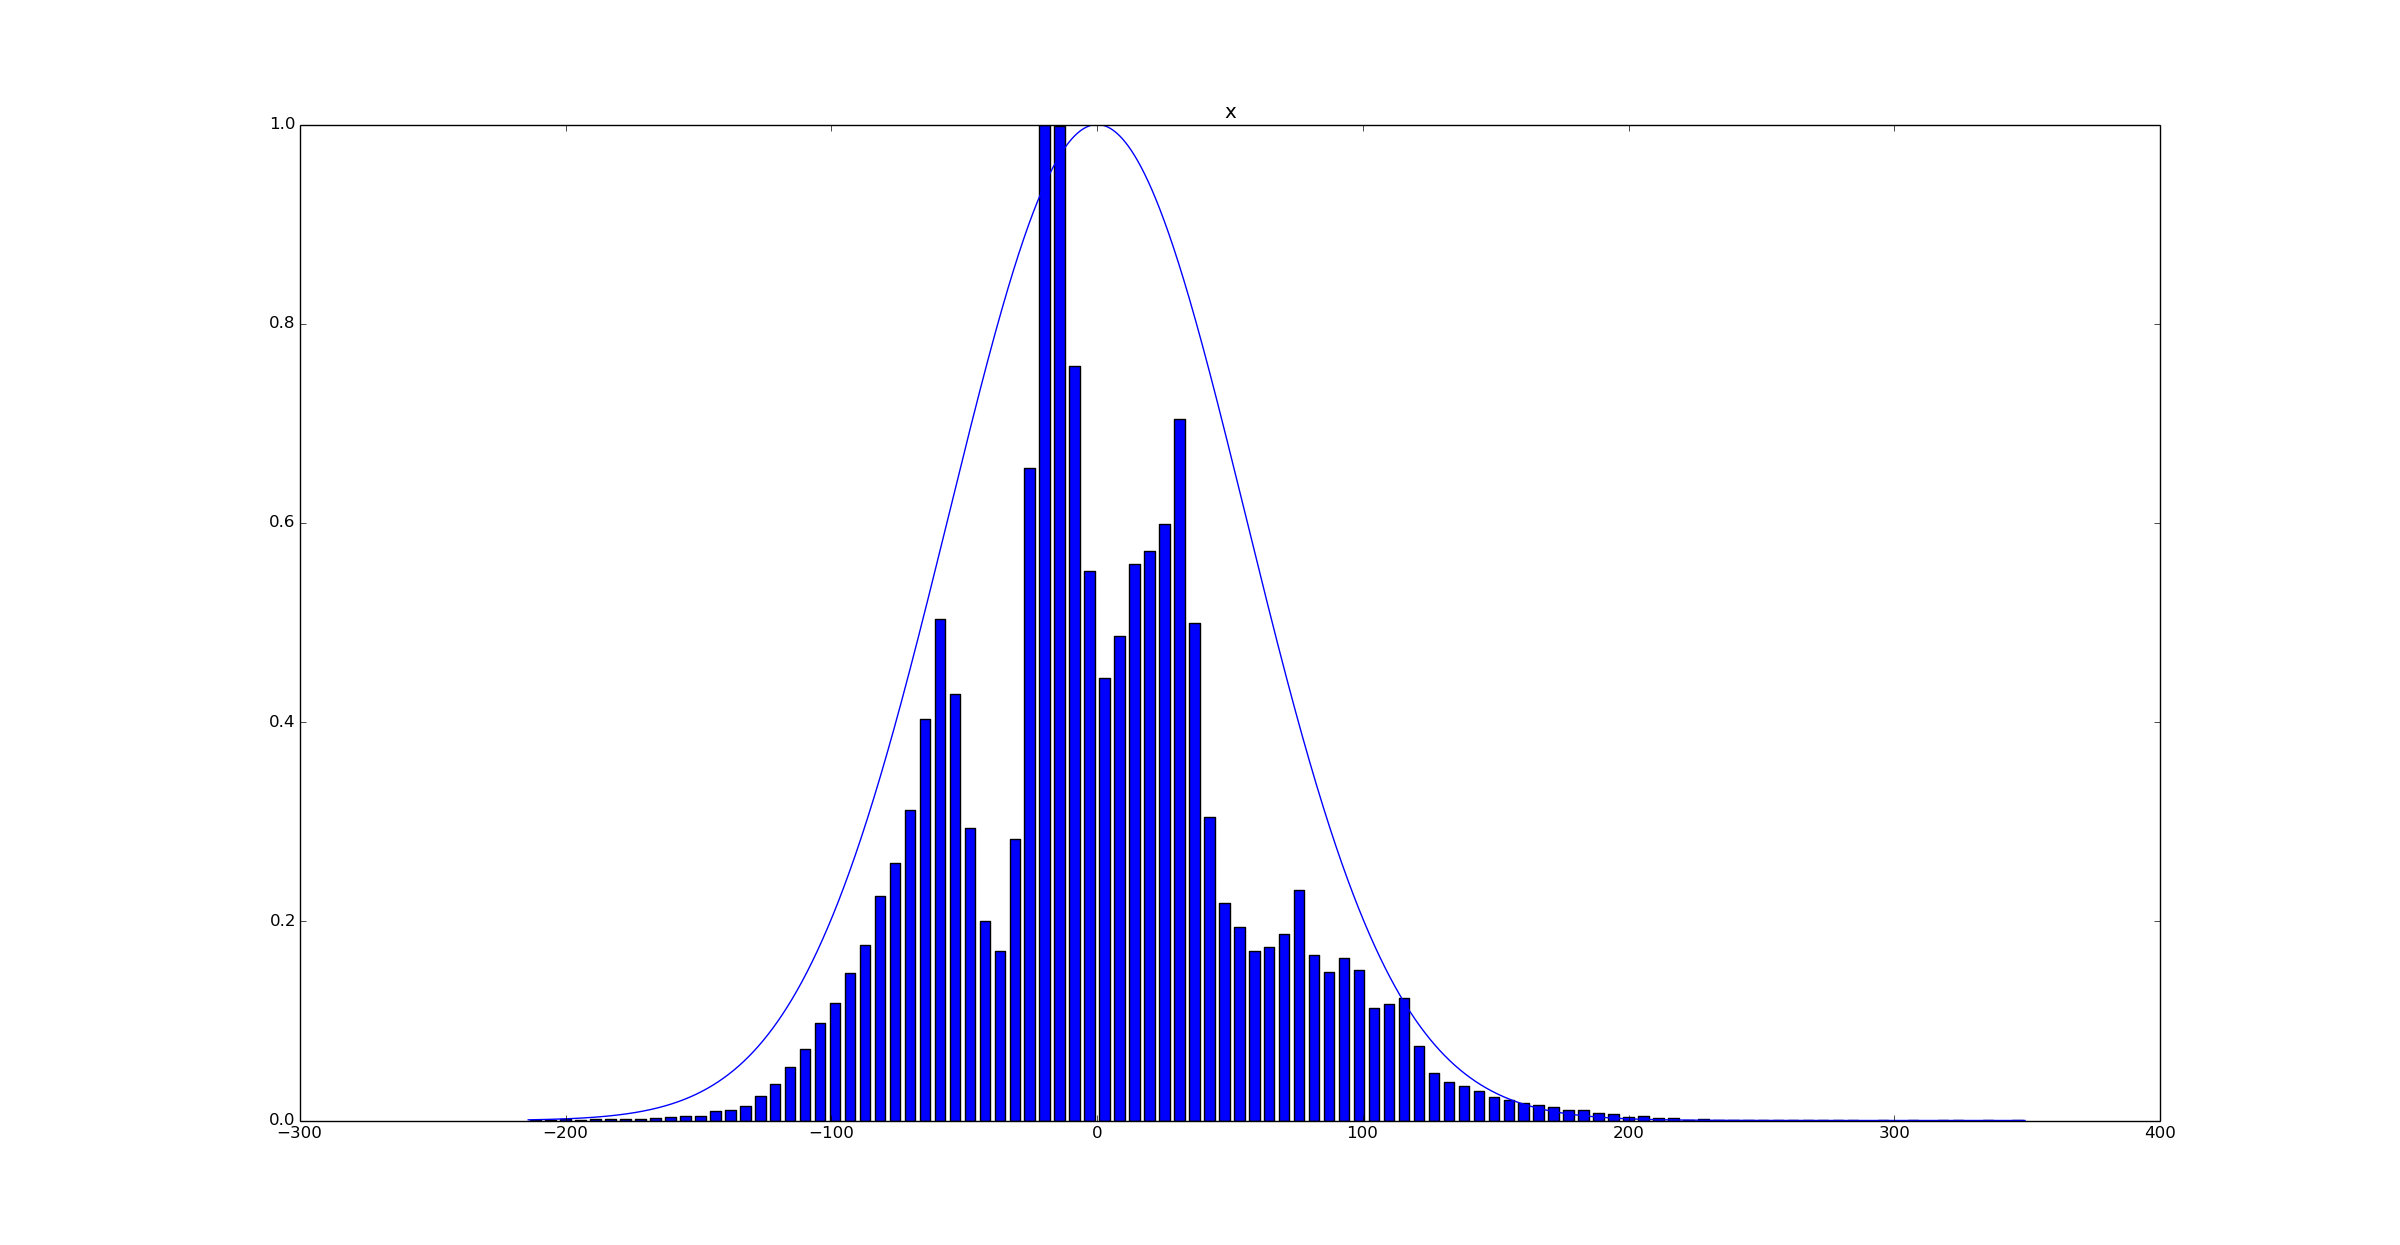
\includegraphics[clip, trim = 120 0 120 0, width=\textwidth]{figures/chapter3/norm_x}
    \caption[Error histogram in the $x$ dimension.]{Error histogram in the $x$ dimension with of $\mu = \SI{-8.89}{\micro \m}$ and $\sigma = \SI{293}{\mm}$.}
  \end{subfigure}
~
  \begin{subfigure}{0.48\textwidth}
     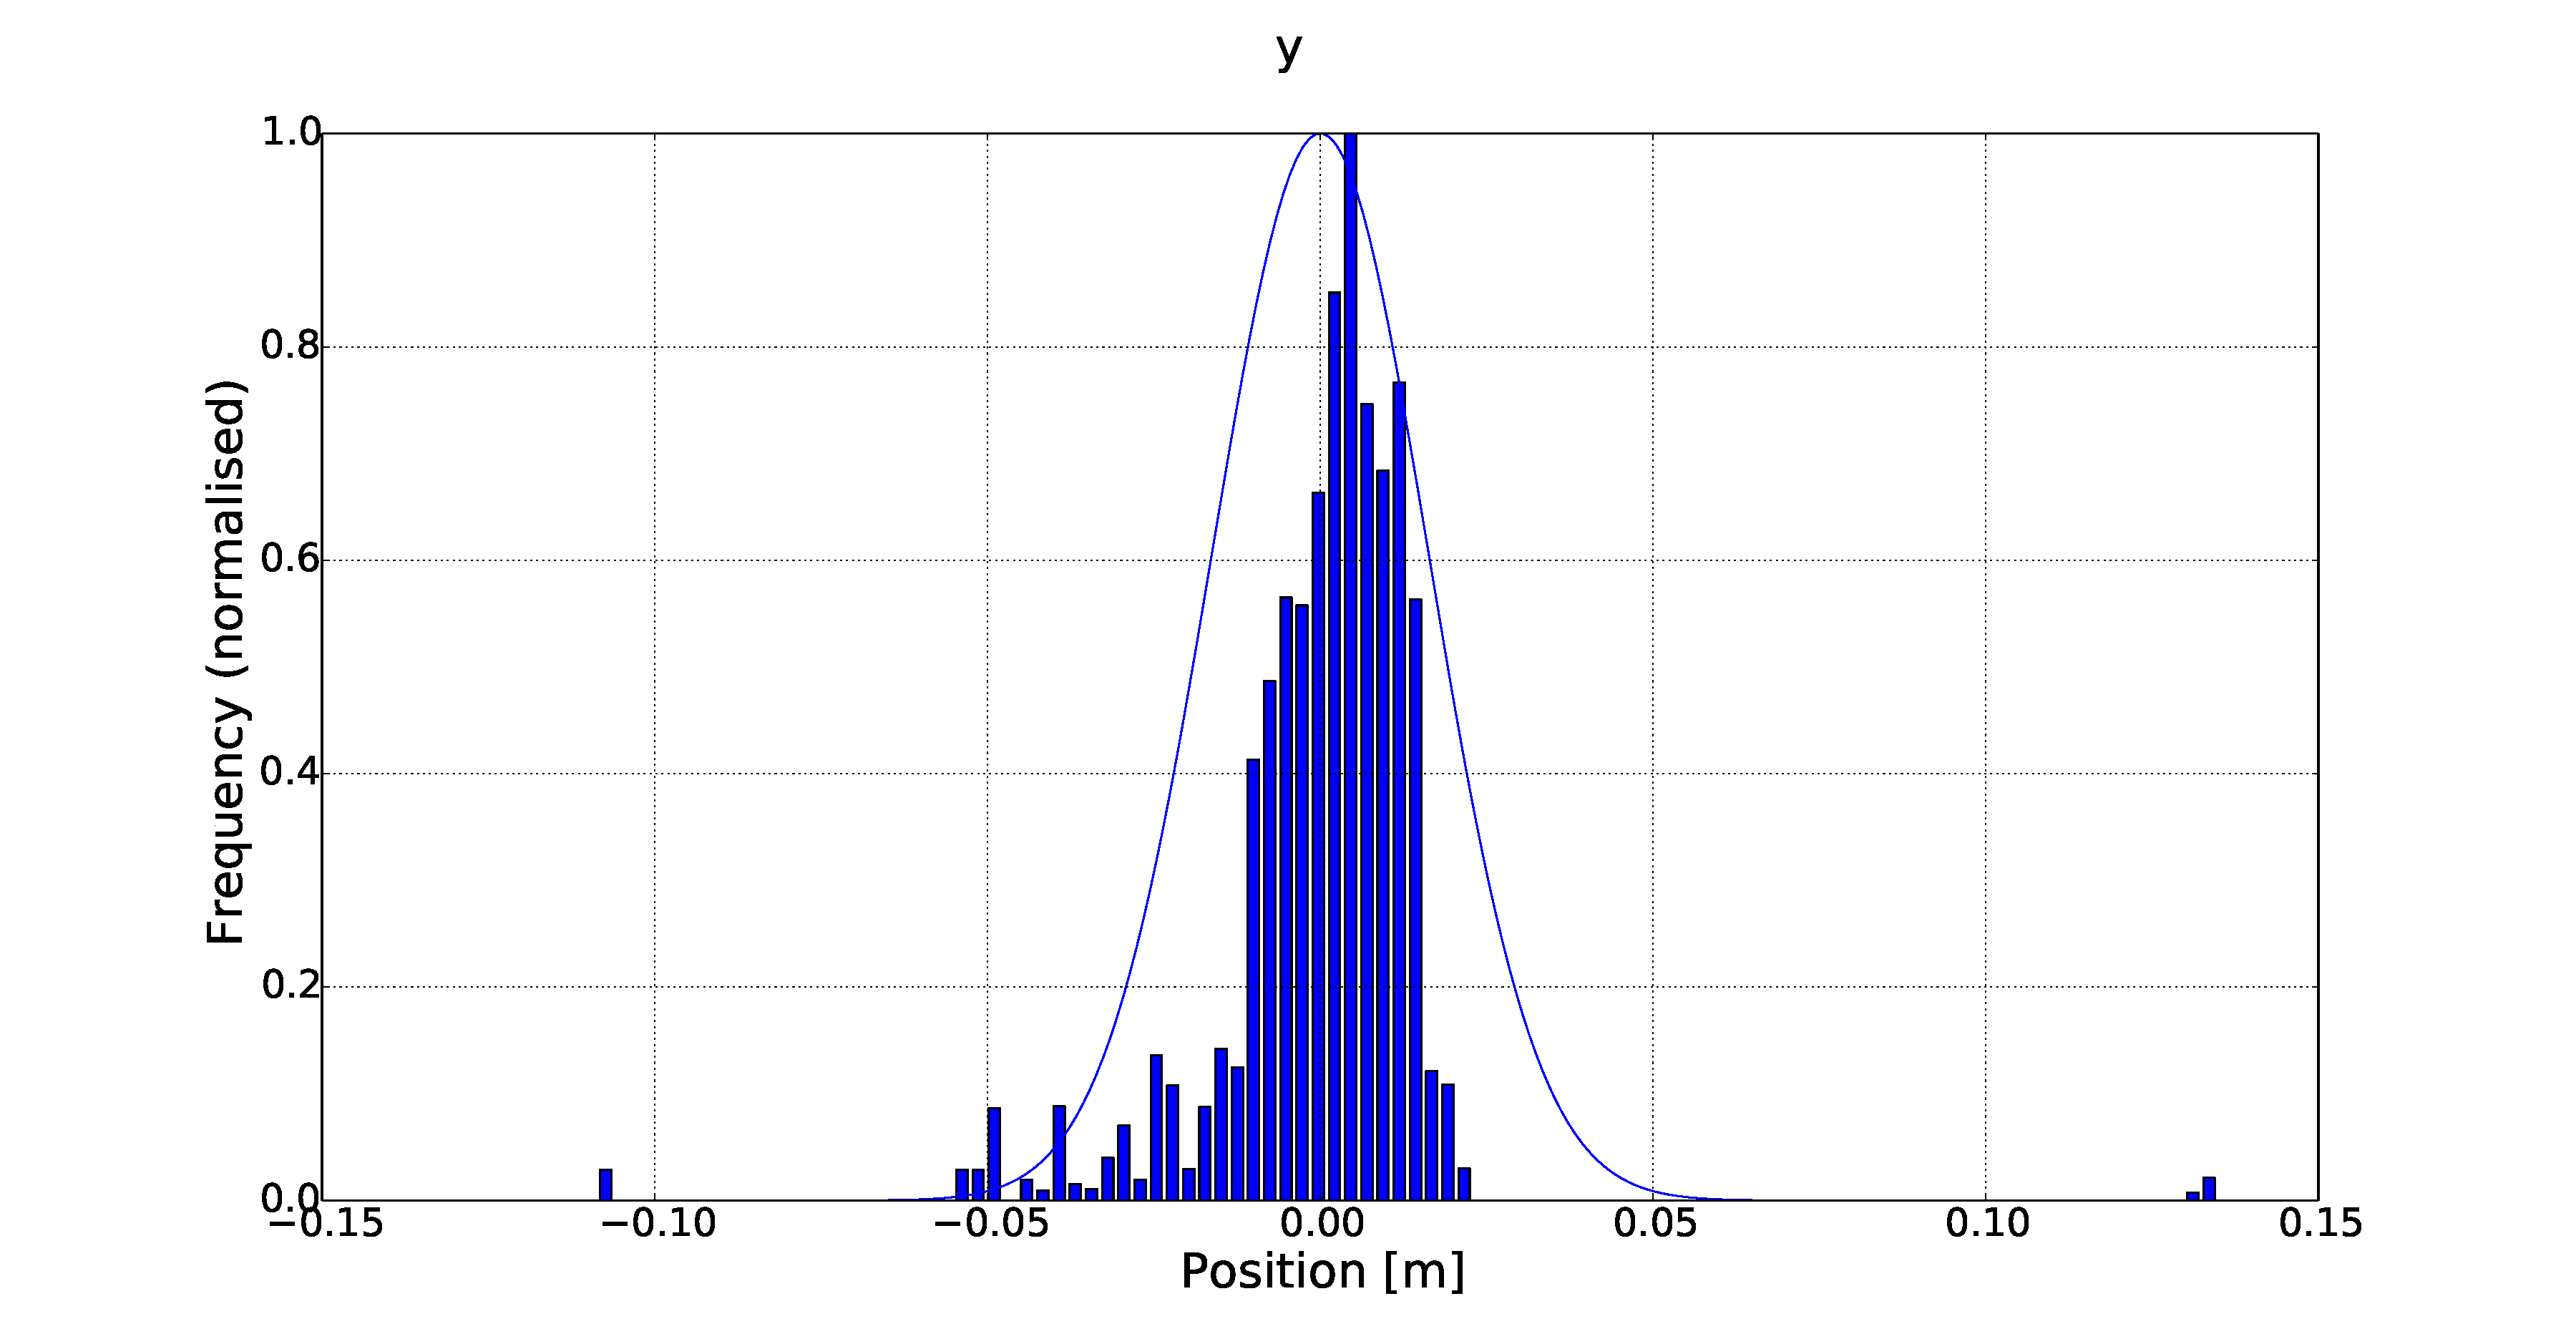
\includegraphics[clip, trim = 120 0 120 0, width=\textwidth]{figures/chapter3/norm_y}
     \caption[Error histogram in the $y$ dimension.]{Error histogram in the $y$ dimension with $\mu = \SI{-10.1}{\micro \m}$ and $\sigma = \SI{167}{\mm}$.}
  \label{fig:norm-y}
  \end{subfigure}

  \begin{subfigure}[t]{0.48\textwidth}
     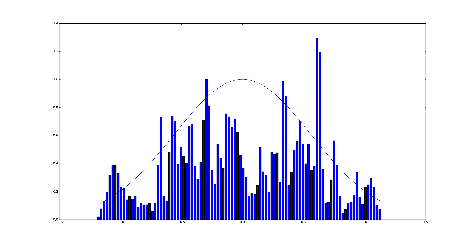
\includegraphics[clip, trim = 120 0 120 0, width=\textwidth]{figures/chapter3/norm_z.pdf}
     \caption[Error histogram in the $z$ dimension.]{Error histogram in the $z$ dimension with $\mu = \SI{1.31}{\mm}$ and $\sigma = \SI{32.5}{\mm}$.}
  \label{fig:norm-z}
  \end{subfigure}
~
  \begin{subfigure}[t]{0.48\textwidth}
     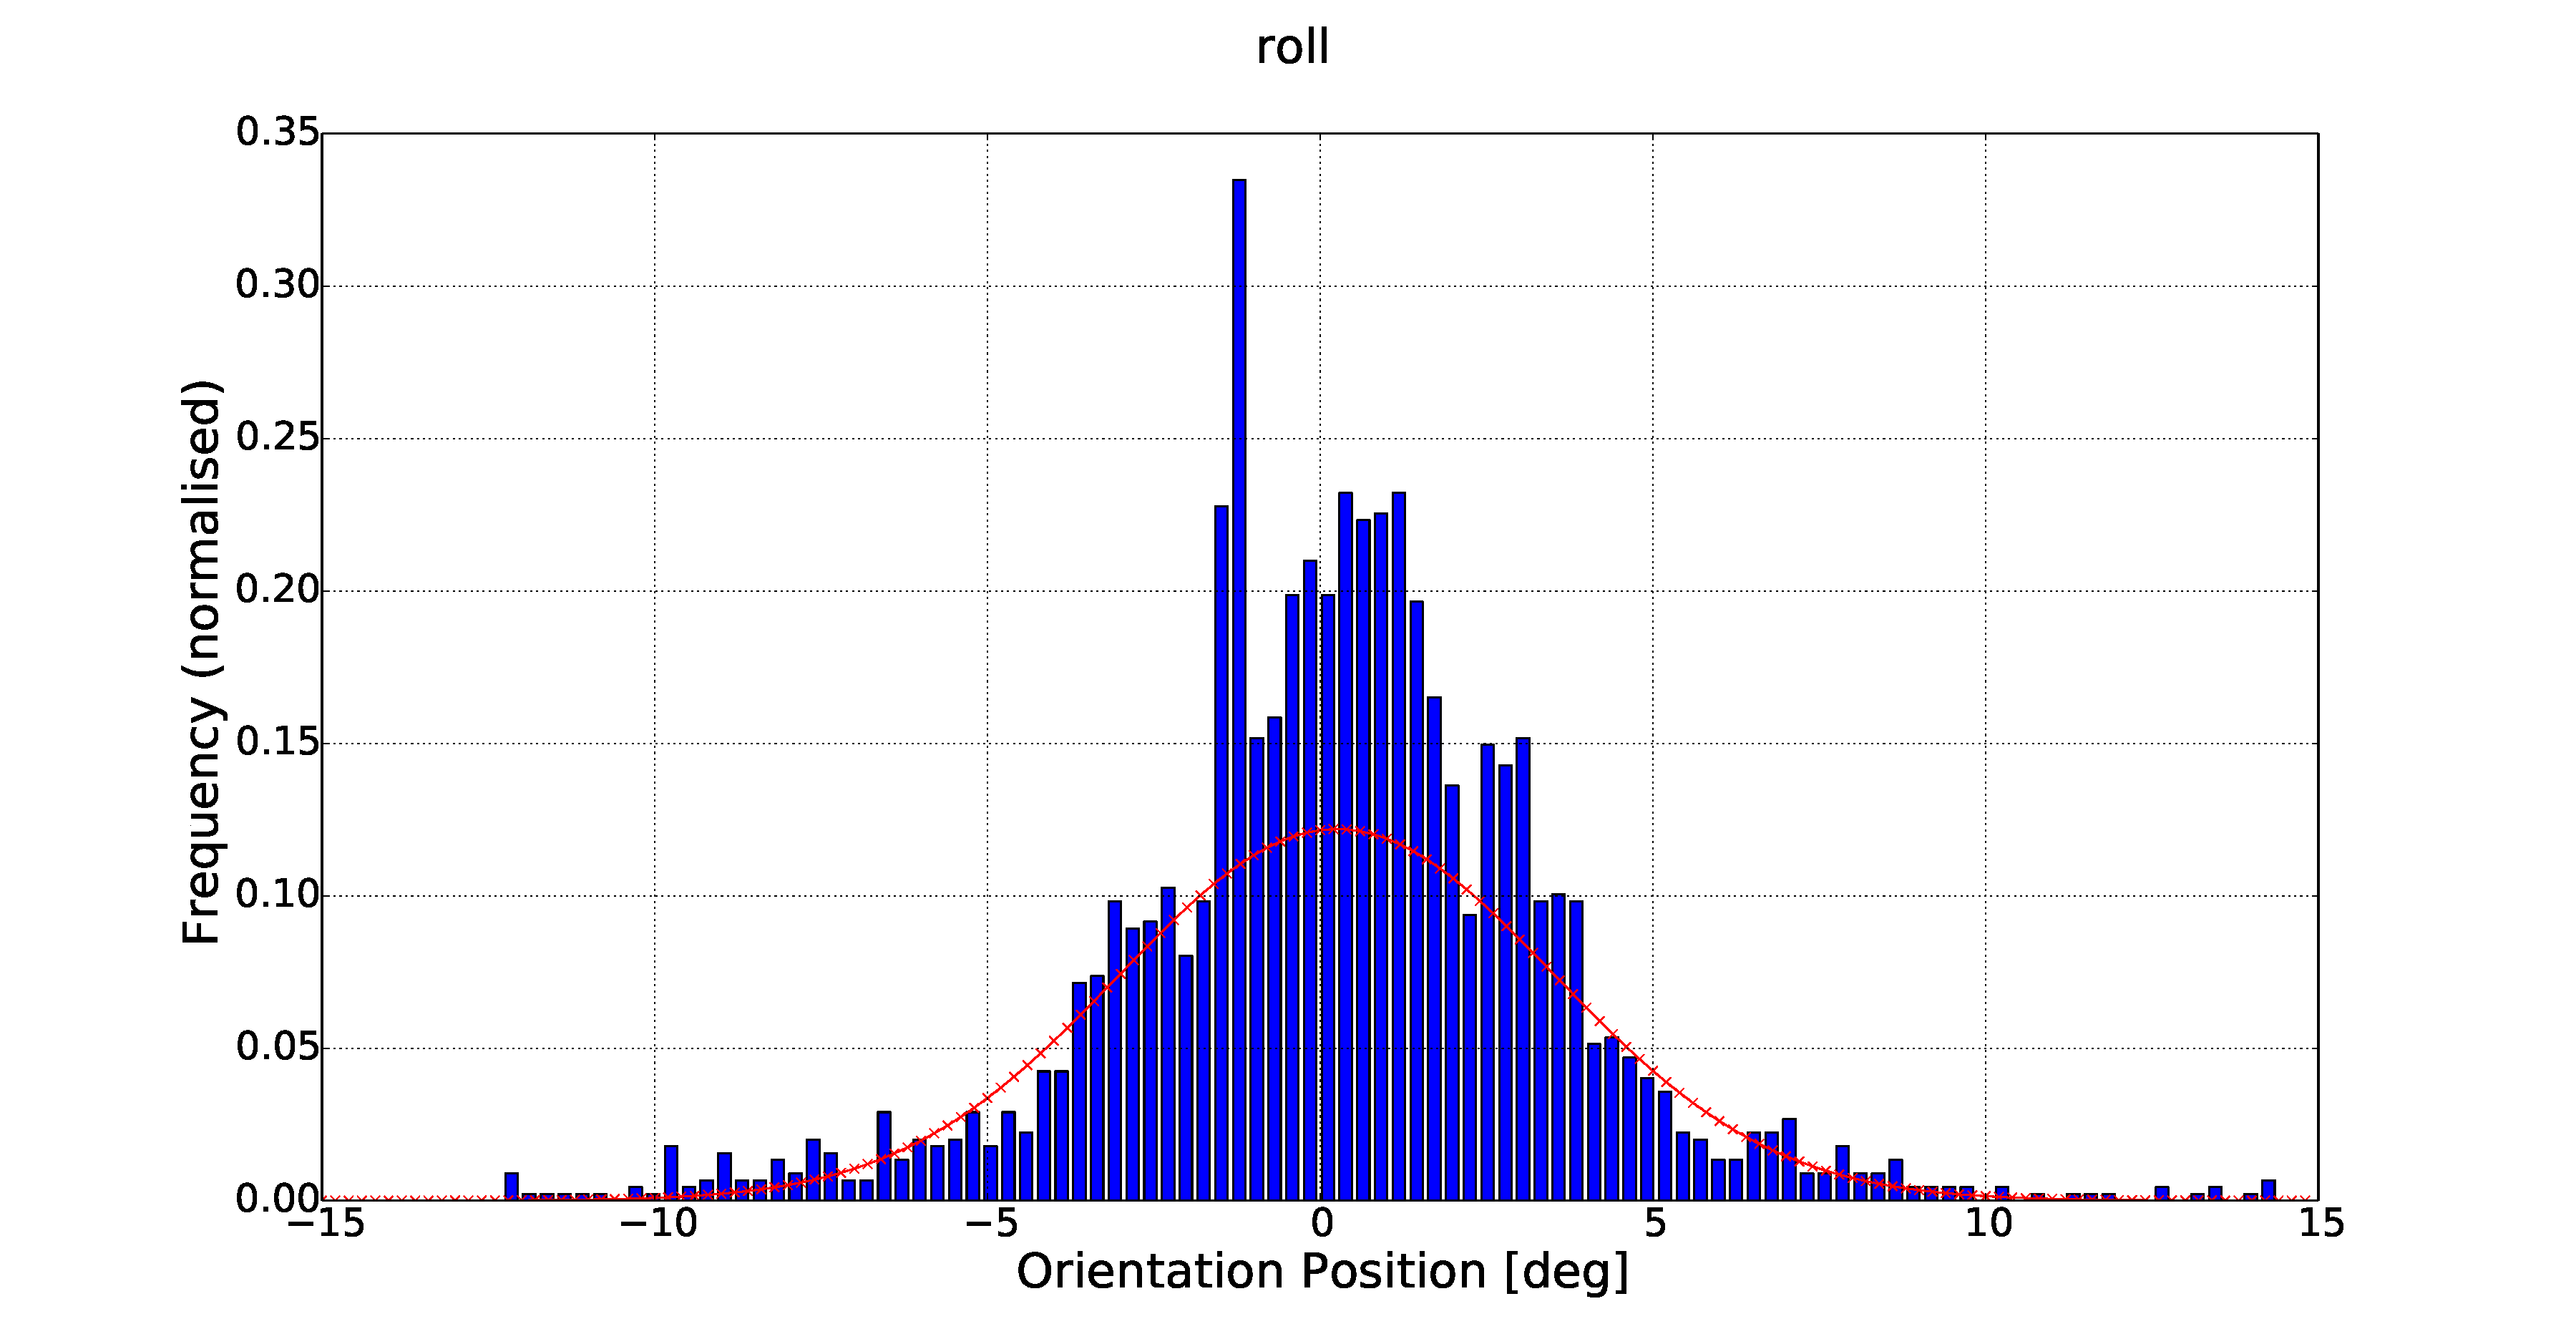
\includegraphics[clip, trim = 120 0 120 0, width=\textwidth]{figures/chapter3/norm_roll.pdf}
     \caption[Error histogram in the roll dimension.]{Error histogram in the roll dimension with $\mu = $ 2 mili-degrees and $\sigma = \ang{8.6}$.}
  \label{fig:norm-roll}
  \end{subfigure}

  \begin{subfigure}{0.48\textwidth}
     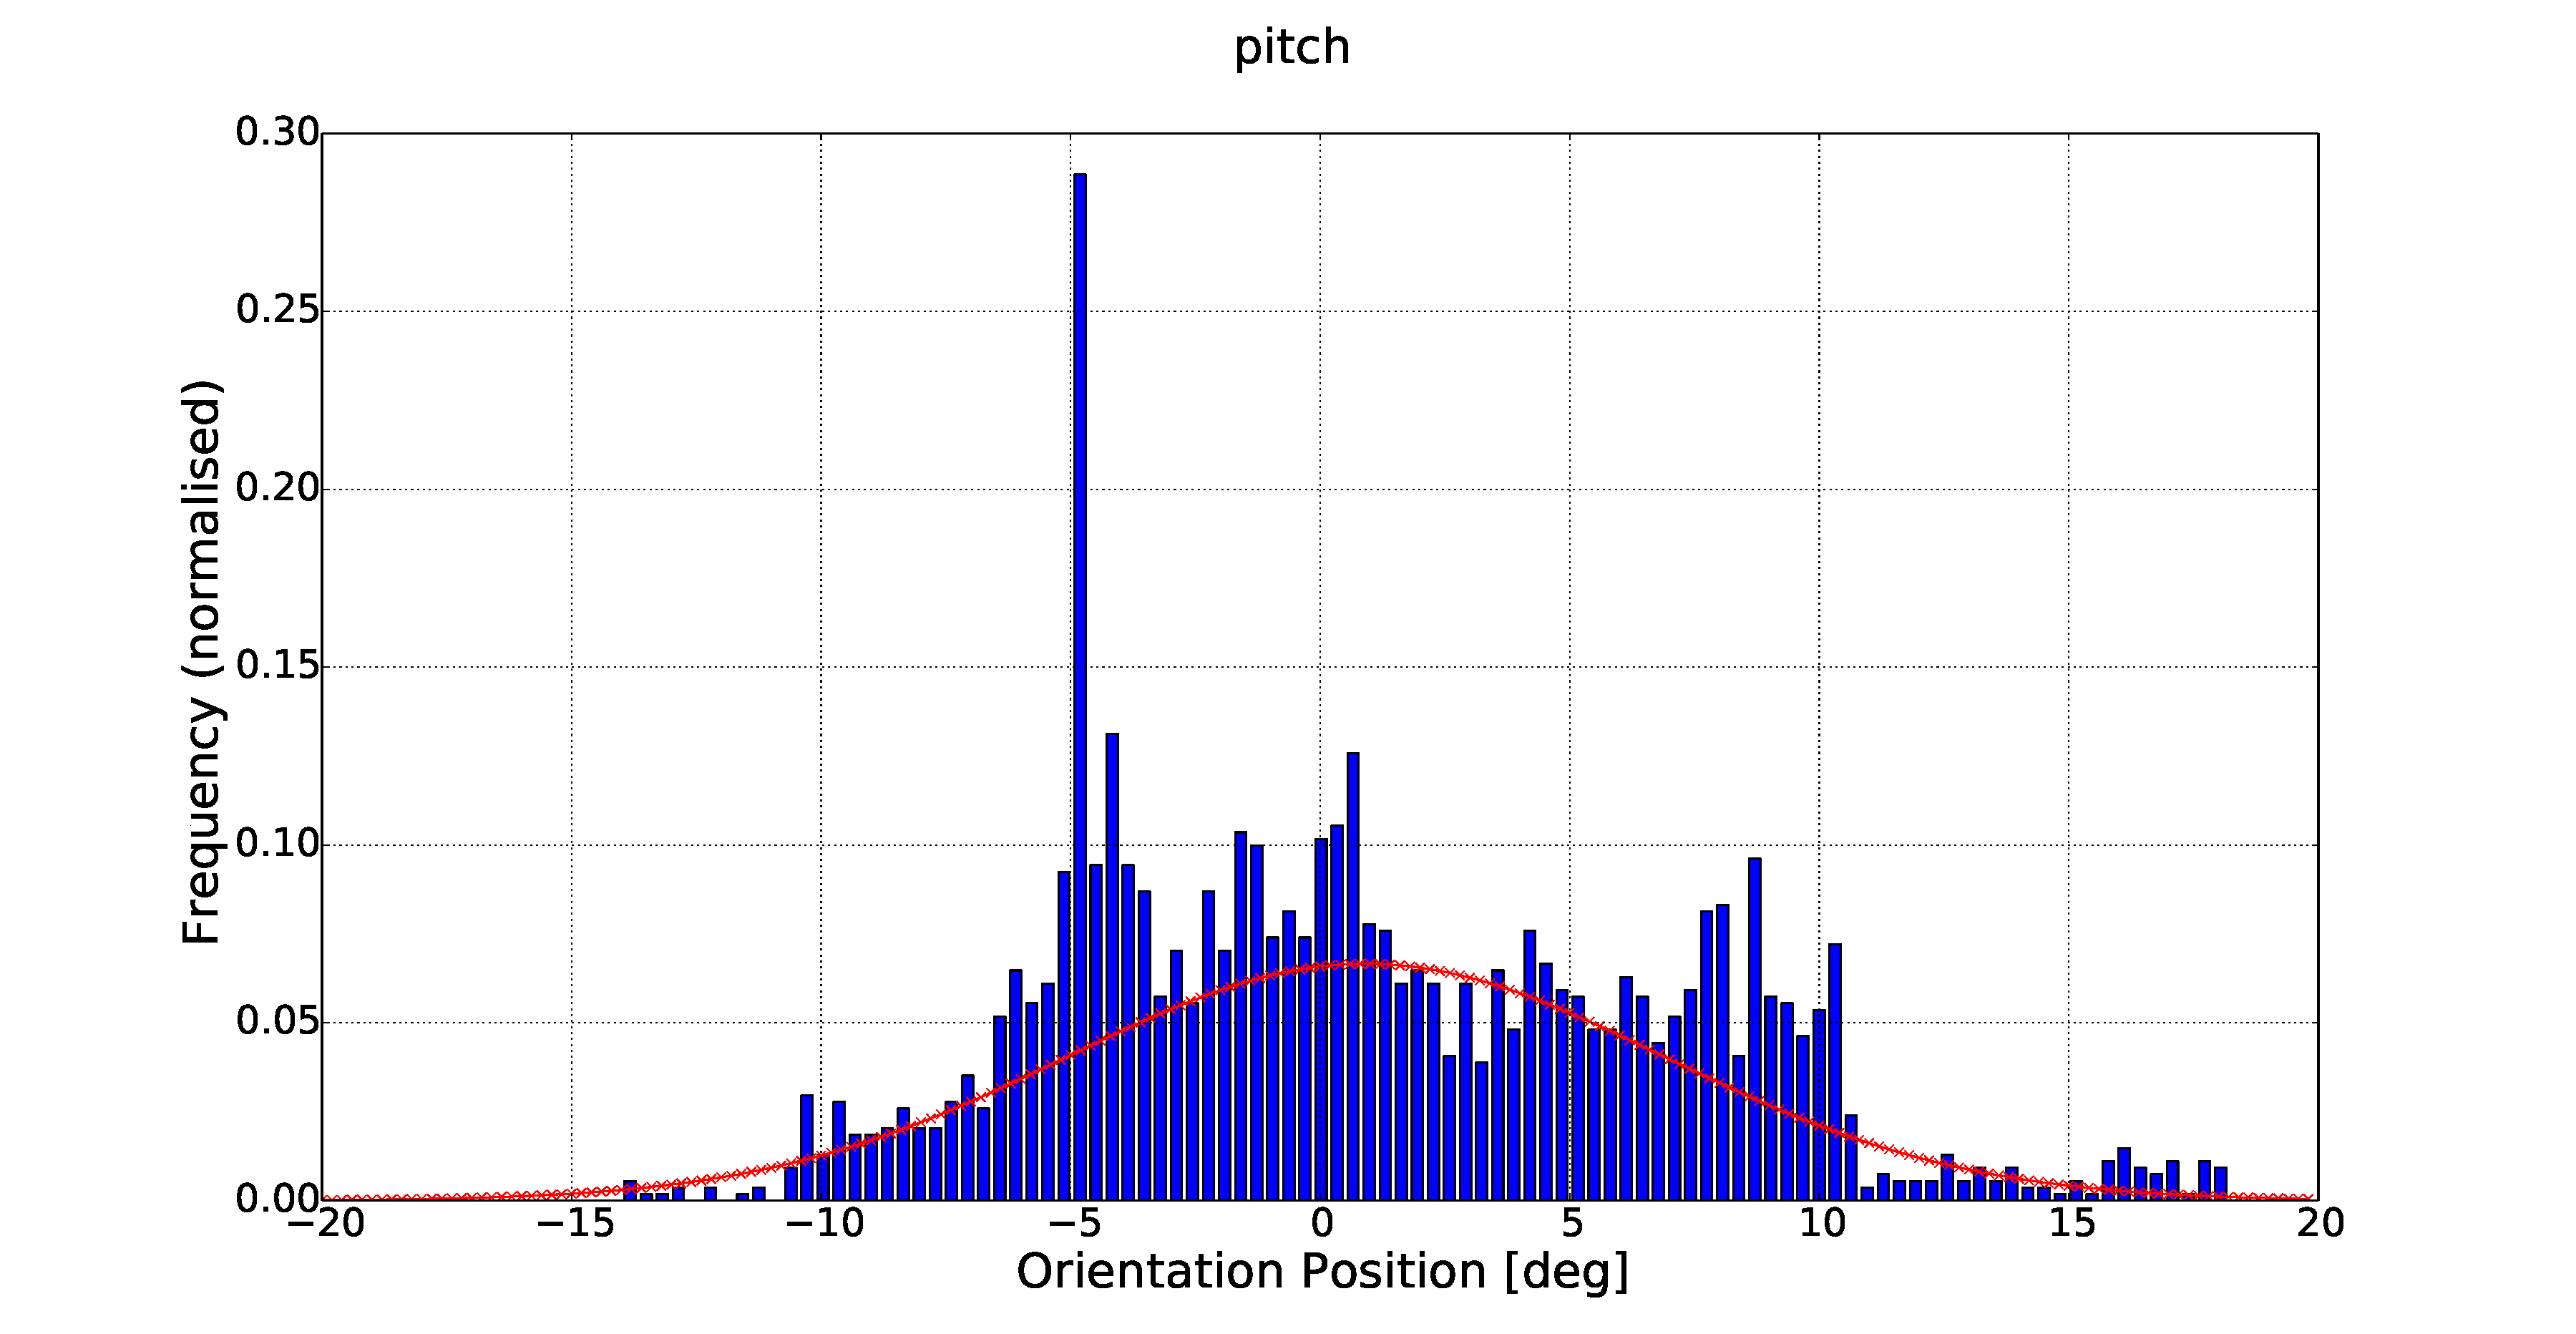
\includegraphics[clip, trim = 120 0 120 0, width=\textwidth]{figures/chapter3/norm_pitch.pdf}
     \caption[Histogram in the pitch dimension.]{Error histogram in the pitch dimension with $\mu = $ 3.8 mili-degrees and $\sigma = \ang{10}$.}
  \label{fig:norm-pitch}
  \end{subfigure}
~
  \begin{subfigure}{0.48\textwidth}
     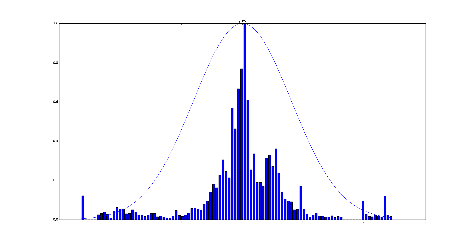
\includegraphics[clip, trim = 120 0 120 0, width=\textwidth]{figures/chapter3/norm_yaw.pdf}
     \caption[Histogram of the yaw dimension.]{Error histogram in the yaw dimension with $\mu = $ 0.14 mili-degrees and $\sigma = \ang{9.73}$. }
  \label{fig:norm-yaw}
  \end{subfigure}
  \caption[Plots of the frequency histograms of the error data in each dimension.]{Plots of the frequency histograms of the error data in each dimension.}
  \label{fig:err-norm}
\end{figure*}

It can be seen that all the plots are roughly centred around zero and are very nearly normally distributed. The $z$ dimension displays the largest standard deviation of approximately 560mm. The reason behind this is the bad depth estimates that a single camera system provides. The standard deviations of the other dimensions are within the range that was expected of the system. However, at first glance, the CVS's does not seem to be as accurate as hoped. 

In all, the frequency histogram and normal distribution plots of the errors in Figure~\ref{fig:err-norm} show that the assumption made in Equation~\ref{eq:chap3-eq2-offset}, that the errors are normally distributed around zero, is a valid one. 

\subsection{Optimum Focal Lengths and Offset}

HERSIEN MEME

As a result of the focal length and offset optimisation procedure, the optimal focal lengths, $f_x$ and $f_y$ were found to be 628 and 535 after 50 iterations of the algorithm, which is considerably less than the optimum of 700 produced by OpenCV's calibration toolbox. Note that these units are given in camera pixel units and not millimetres.

The optimal offset $\bar{\bm{P}}$ was found and is given in Equation~\ref{eq:chap3-offset-value}.

\begin{equation}
  \label{eq:chap3-offset-value}
  \bar{\bm{P}} = 
  \begin{bmatrix}
    240.8mm & 40.09mm & 375.9mm & \ang{184.3} & \ang{-2.697} & \ang{-179.9}
  \end{bmatrix}^T
\end{equation}

The values in $\bar{\bm{P}}$ contain any constant error bias, as well as marker placement errors that may have been introduced to the Vicon test during the measurement process. The large offsets of $\pm\ang{180}$ in the $\theta$ and $\psi$ dimensions can be explained by the differing axis orientations of the CVS camera and Vicon systems, where the axes needed rotating to coincide with one another. This indicates that the offset was correctly calculated and is working as expected. The large offset in the $z$ dimension is to be expected, since single camera's are known to produce very bad depth estimates. However, the relatively large offset of 240mm in the $x$ dimension is slightly surprising, but may be explained if the CVS's camera was placed approximately 240mm from the Vicon system's origin. 

All of the above produce an error two-norm of approximately 0.81 (normalised), compared to the original 1.15 (normalised), showing an overall reduction in the error vector magnitude. Figure~\ref{fig:estimate} shows the results of the Vicon measurements compared to the original and improved CVS measurements in all six dimensions.

\begin{figure*}
  \begin{subfigure}{0.45\textwidth}
    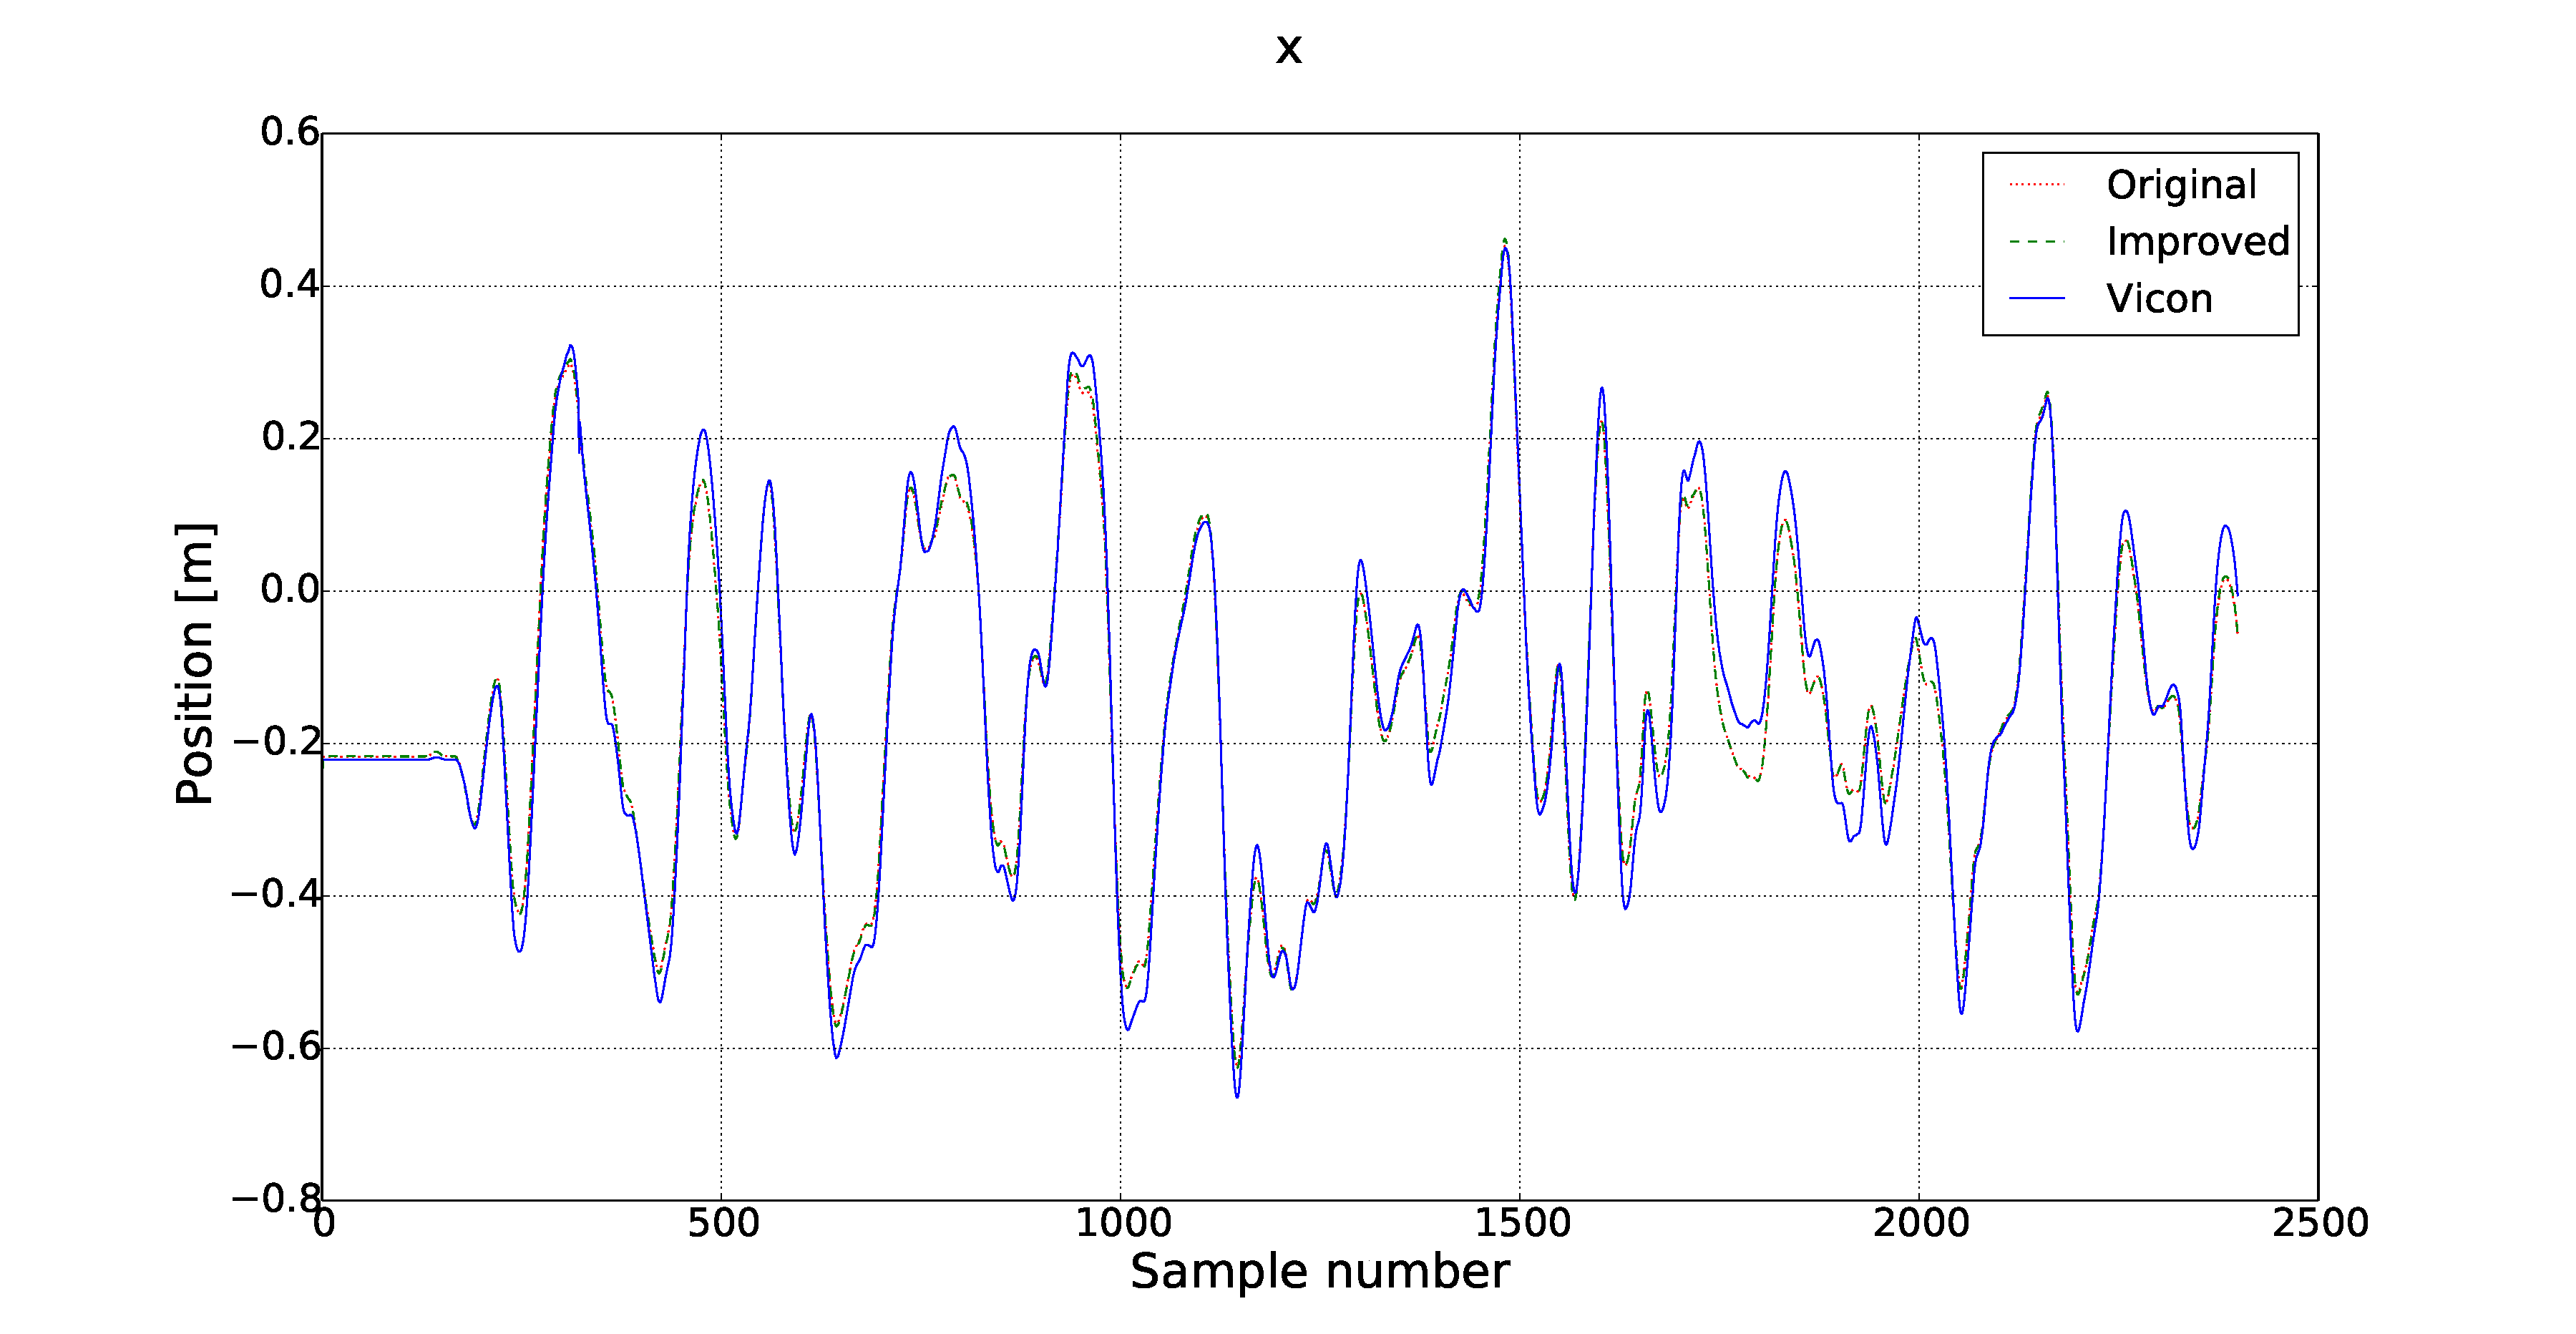
\includegraphics[width=\textwidth]{figures/chapter3/x}
    \caption{The ground-truth Vicon pose estimate, versus the original and improved CV pose estimates in the $x$ dimension.}
  \label{fig:estimate-x}
  \end{subfigure}
~
  \begin{subfigure}{0.45\textwidth}
    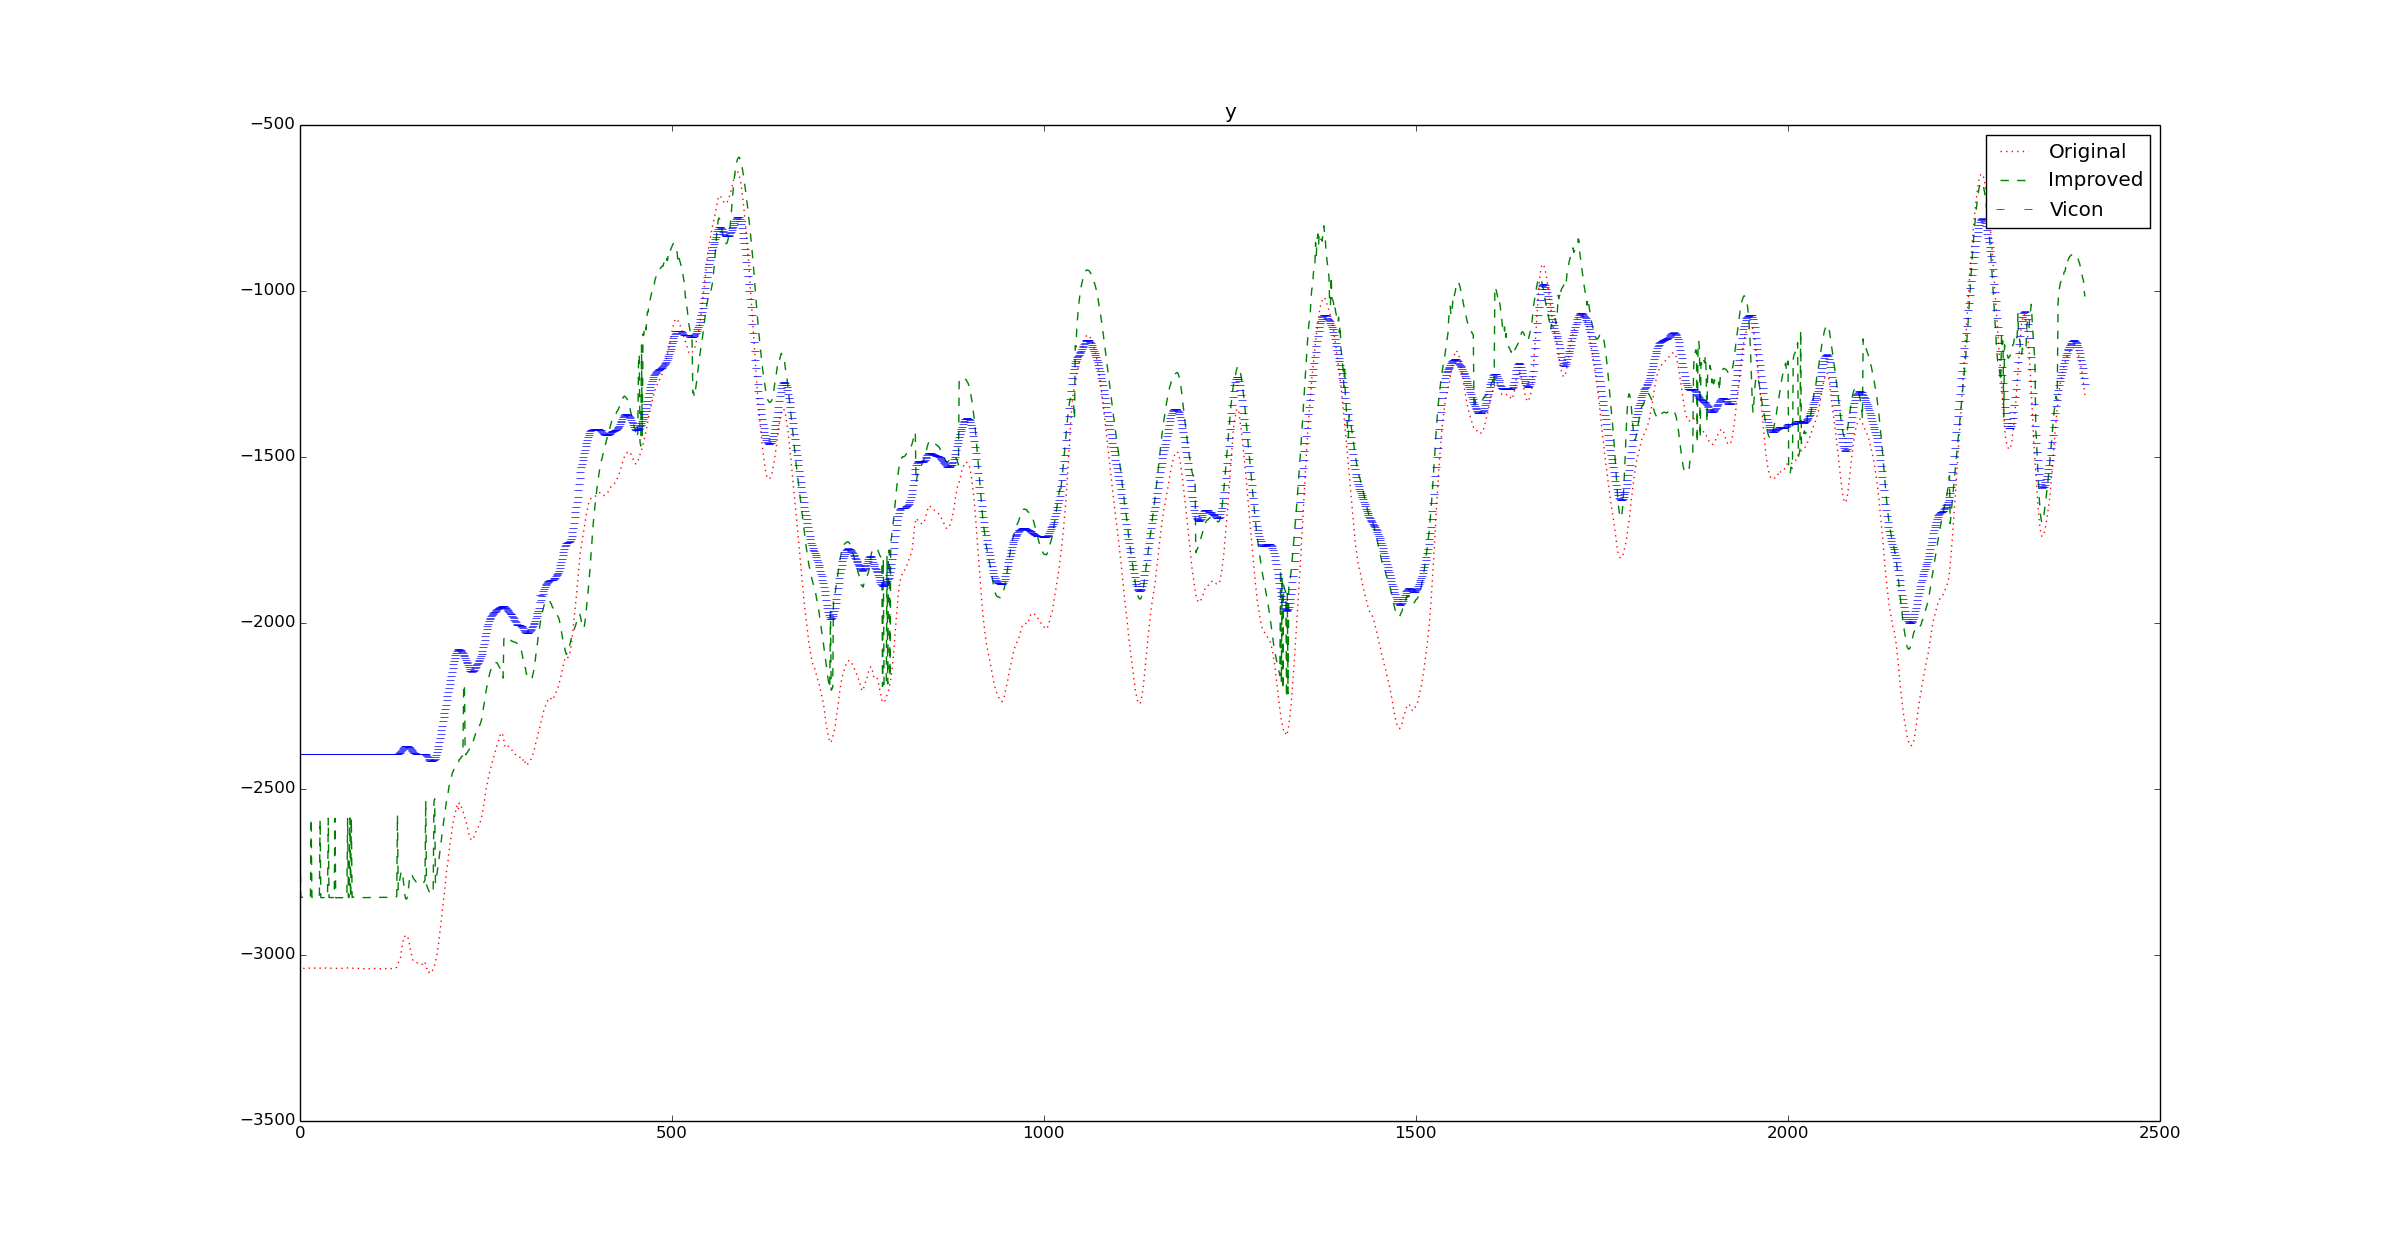
\includegraphics[width=\textwidth]{figures/chapter3/y}
    \caption{The ground-truth Vicon pose estimate, versus the original and improved CV pose estimates in the $y$ dimension.}
  \label{fig:estimate-y}
  \end{subfigure}

  \begin{subfigure}{0.45\textwidth}
    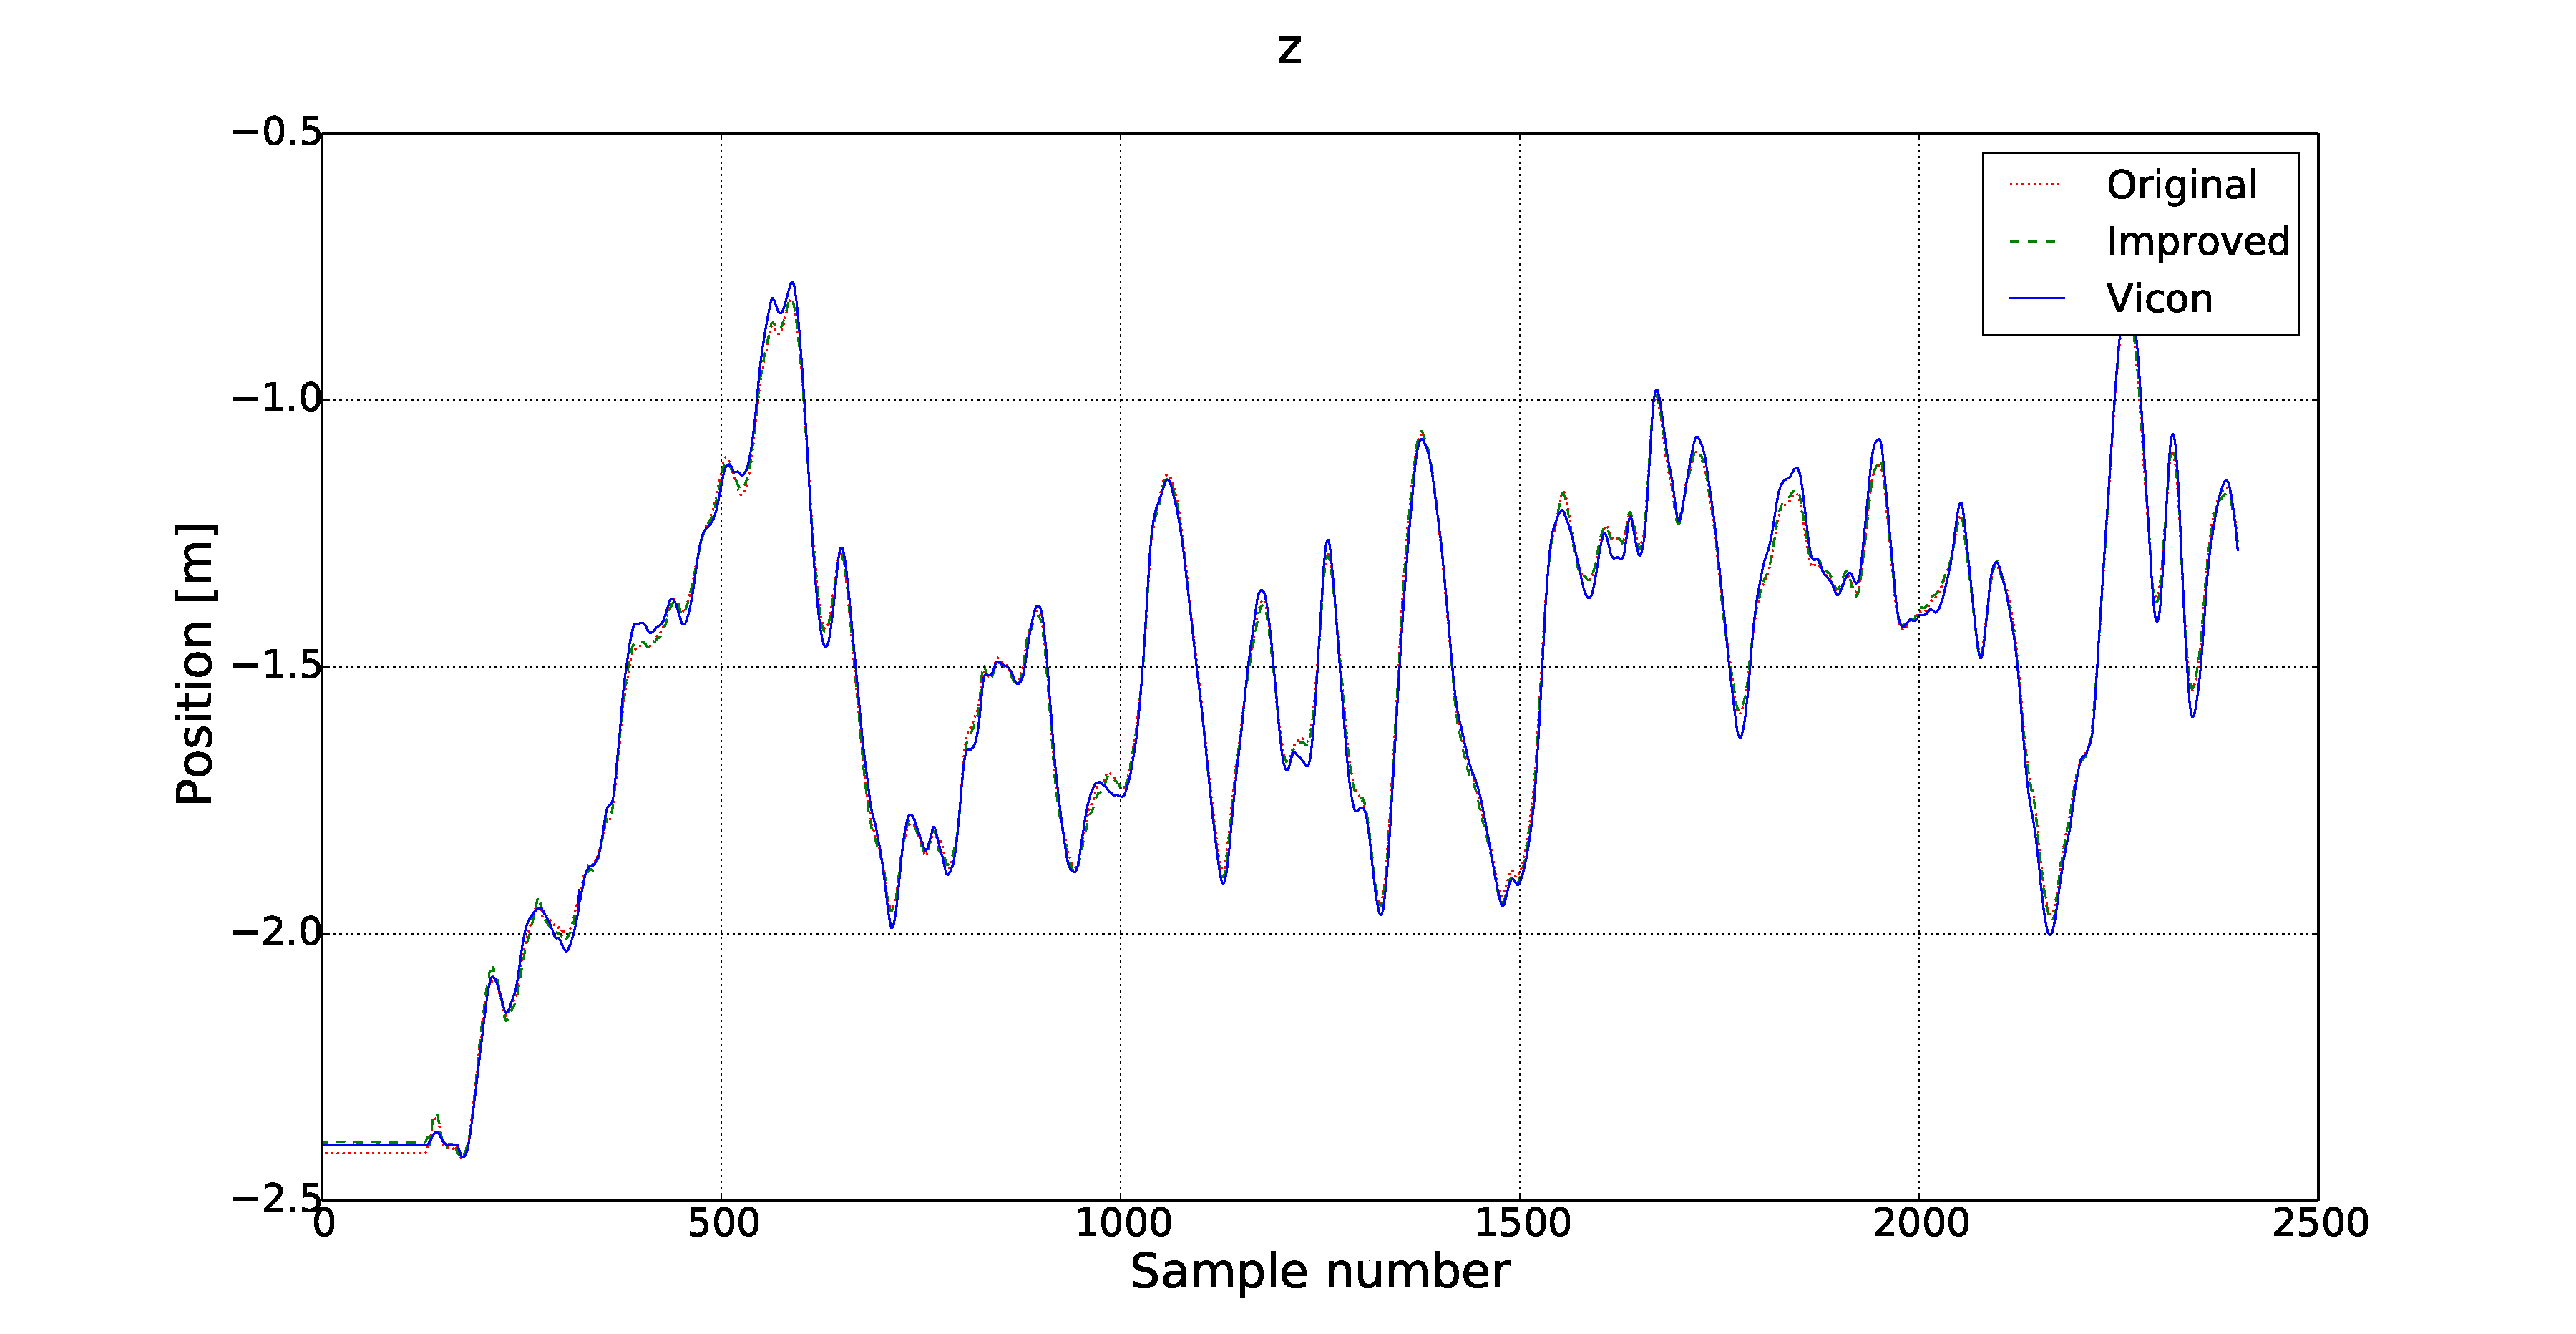
\includegraphics[width=\textwidth]{figures/chapter3/z}
    \caption{The ground-truth Vicon pose estimate, versus the original and improved CV pose estimates in the $z$ dimension.}
  \label{fig:estimate-z}
  \end{subfigure}
~
  \begin{subfigure}{0.45\textwidth}
    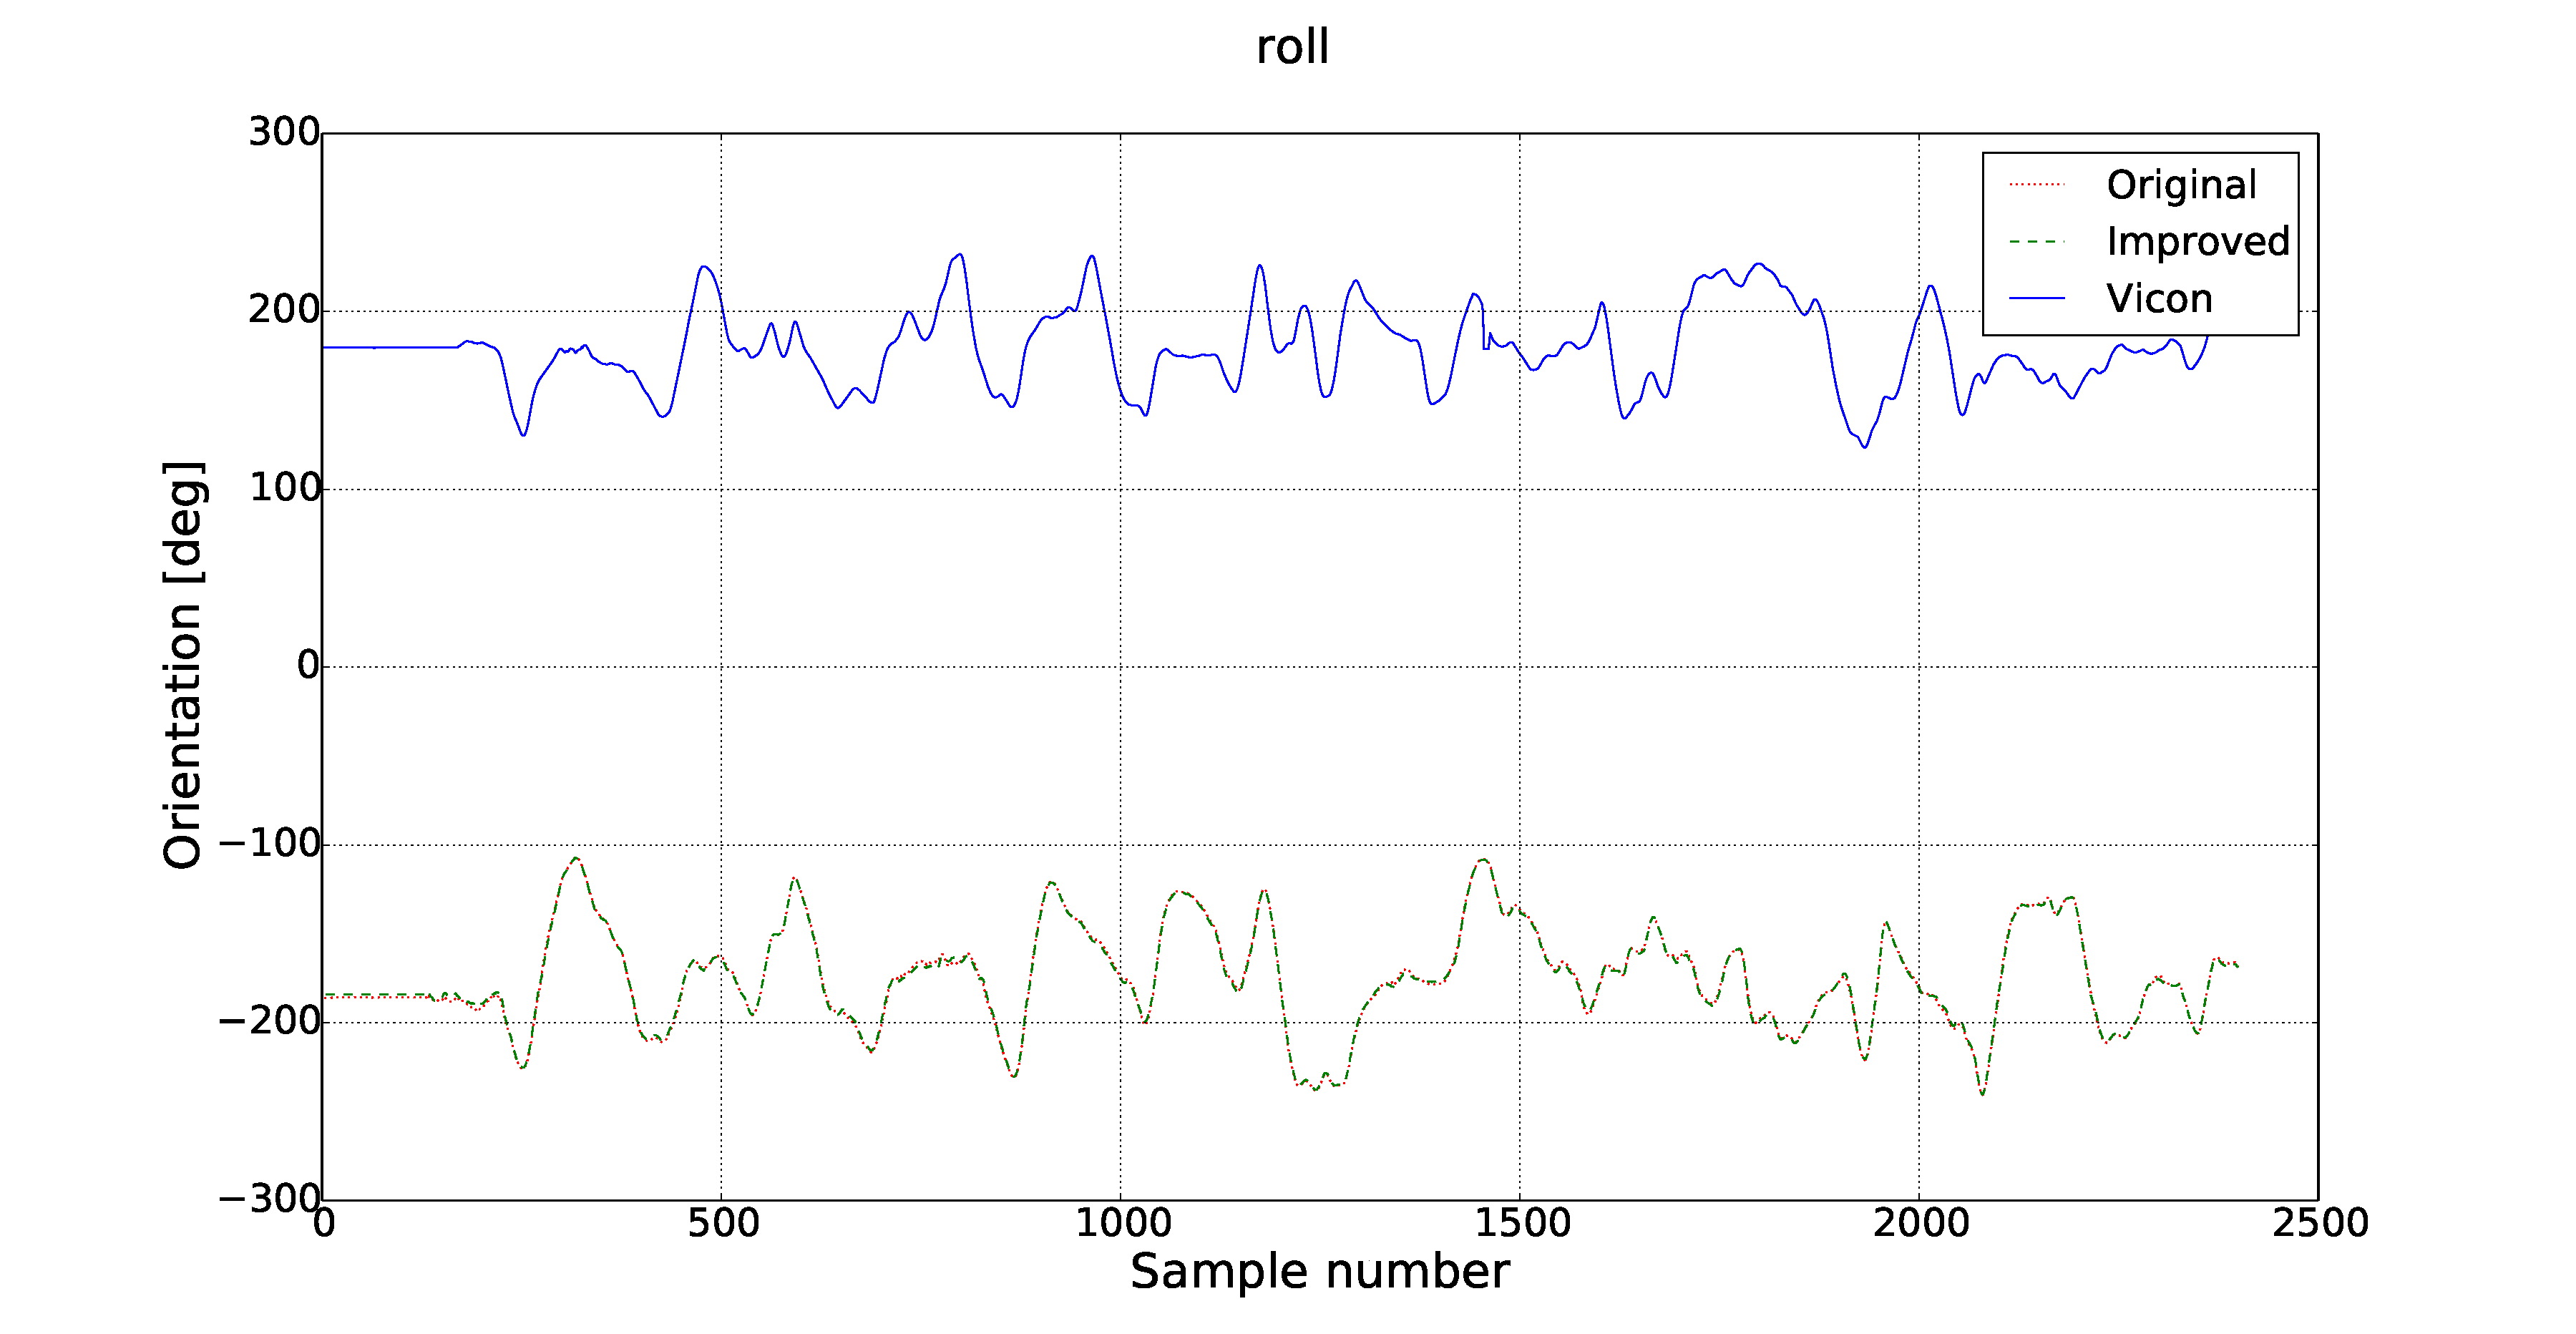
\includegraphics[width=\textwidth]{figures/chapter3/roll}
    \caption{The ground-truth Vicon pose estimate, versus the original and improved CV pose estimates in the $\theta$ dimension.}
  \label{fig:estimate-roll}
  \end{subfigure}

  \begin{subfigure}{0.45\textwidth}
    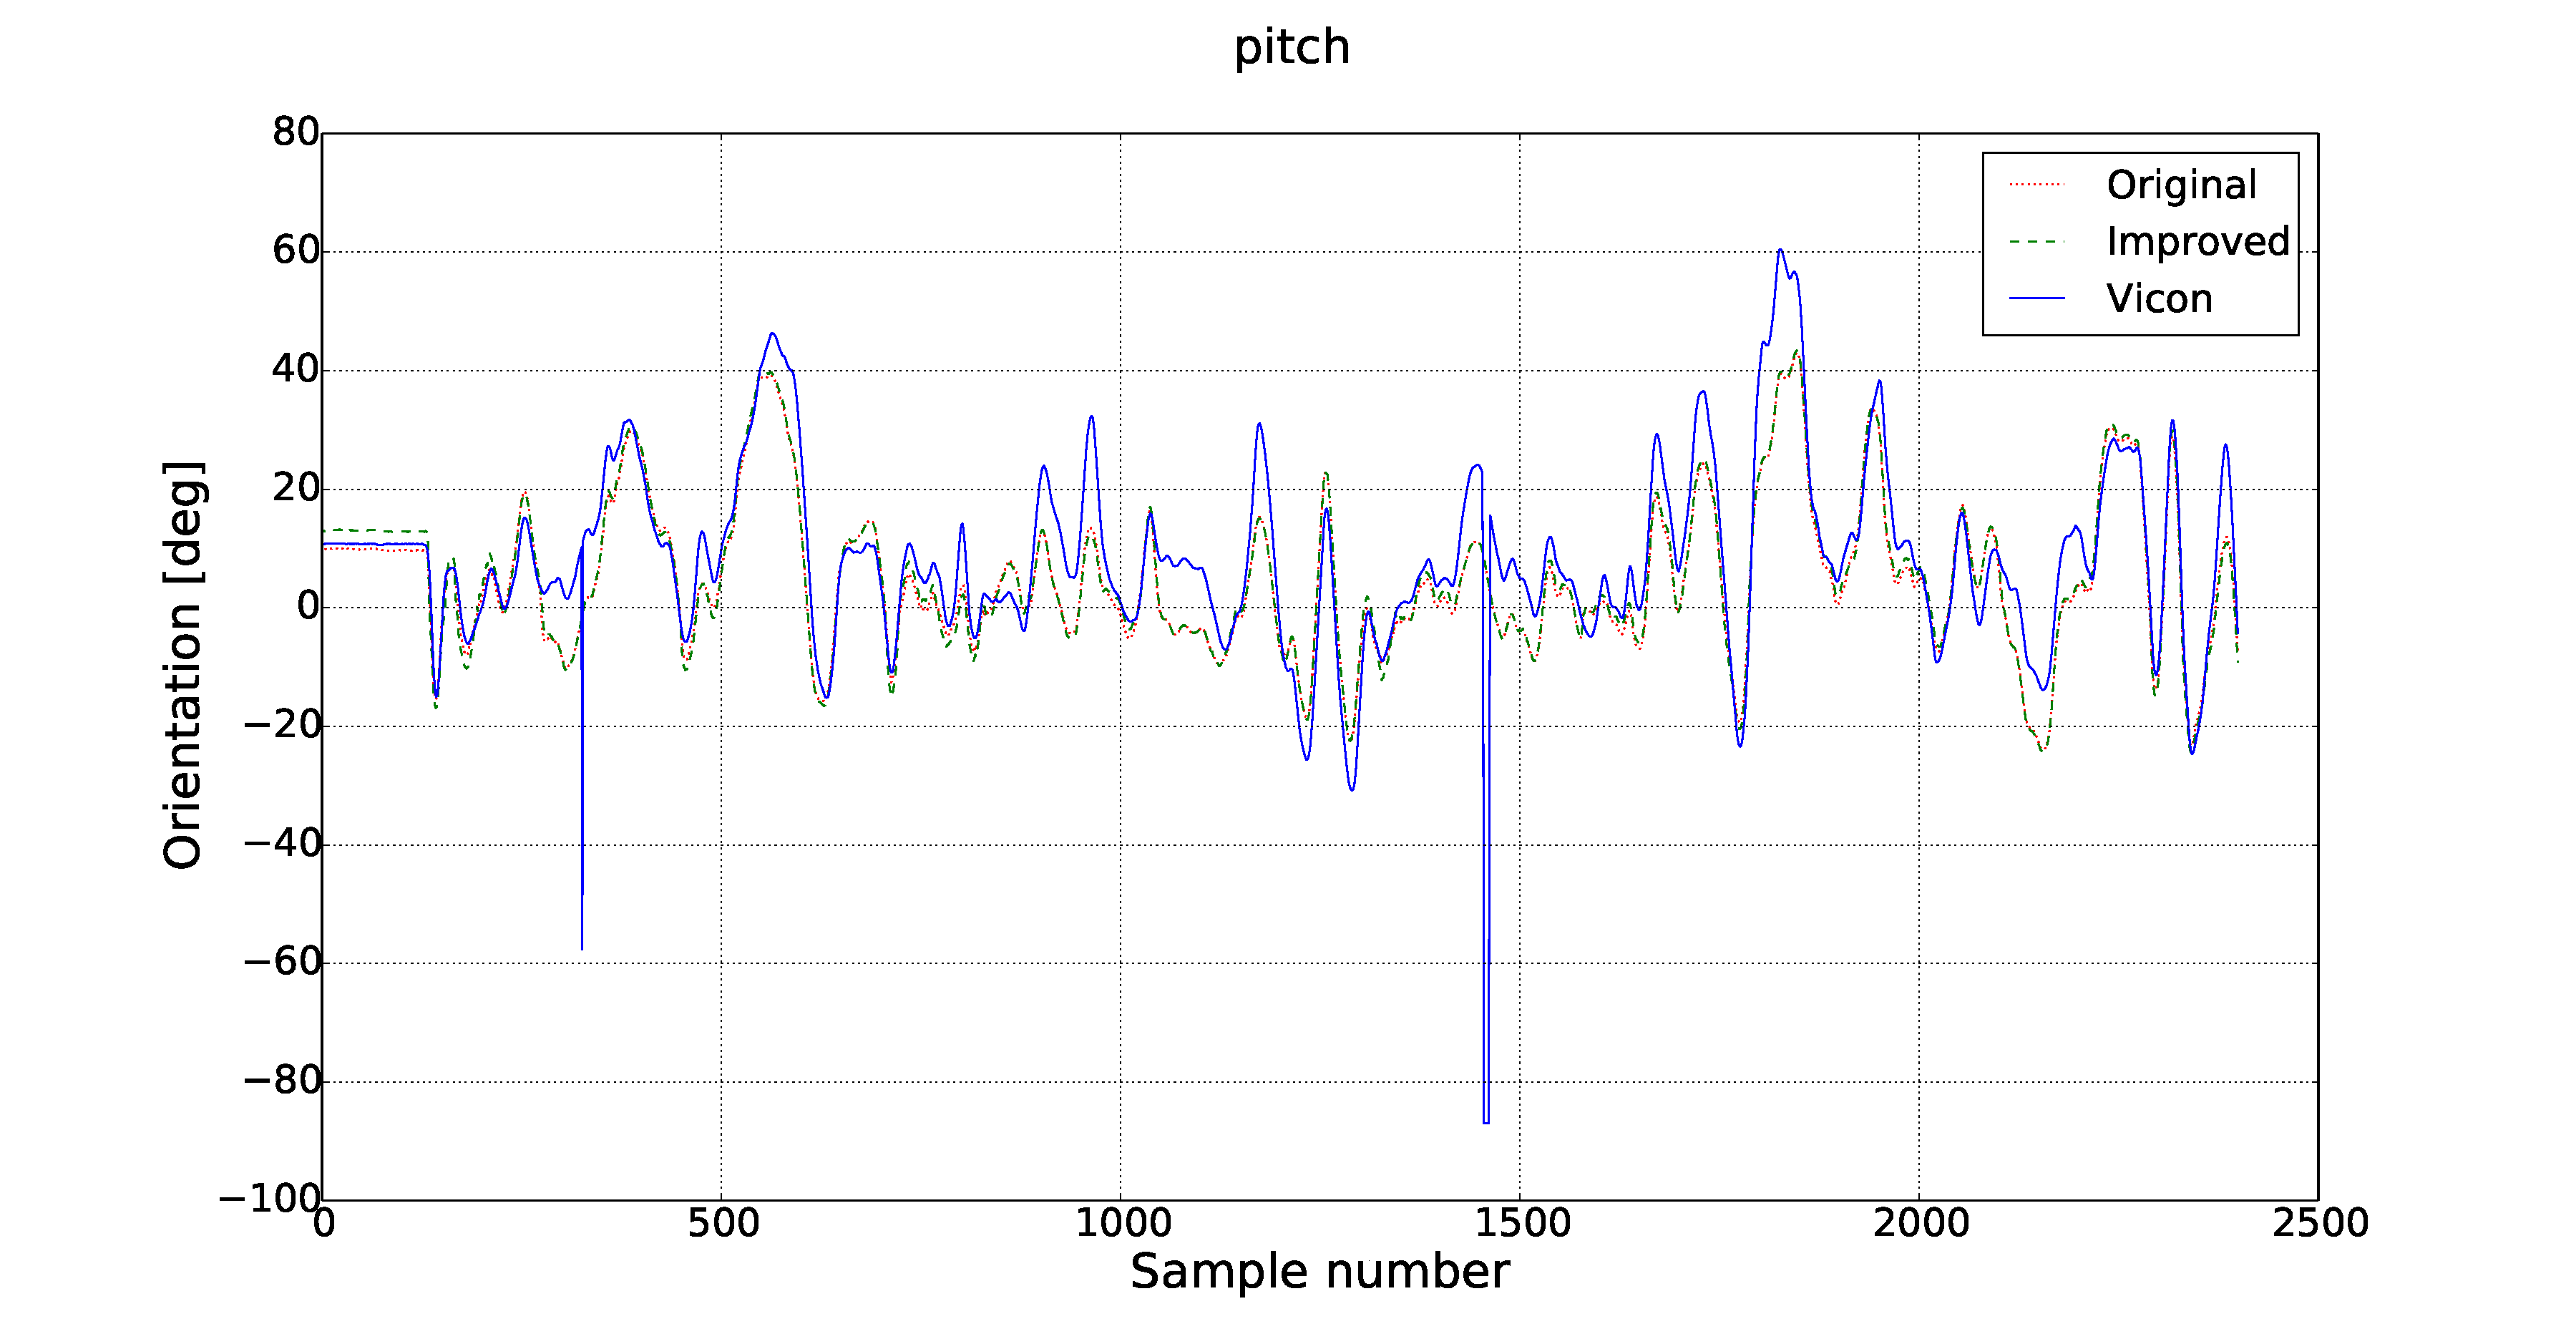
\includegraphics[width=\textwidth]{figures/chapter3/pitch}
    \caption{The ground-truth Vicon pose estimate, versus the original and improved CV pose estimates in the $\phi$ dimension.}
  \label{fig:estimate-pitch}
  \end{subfigure}
~
  \begin{subfigure}{0.45\textwidth}
    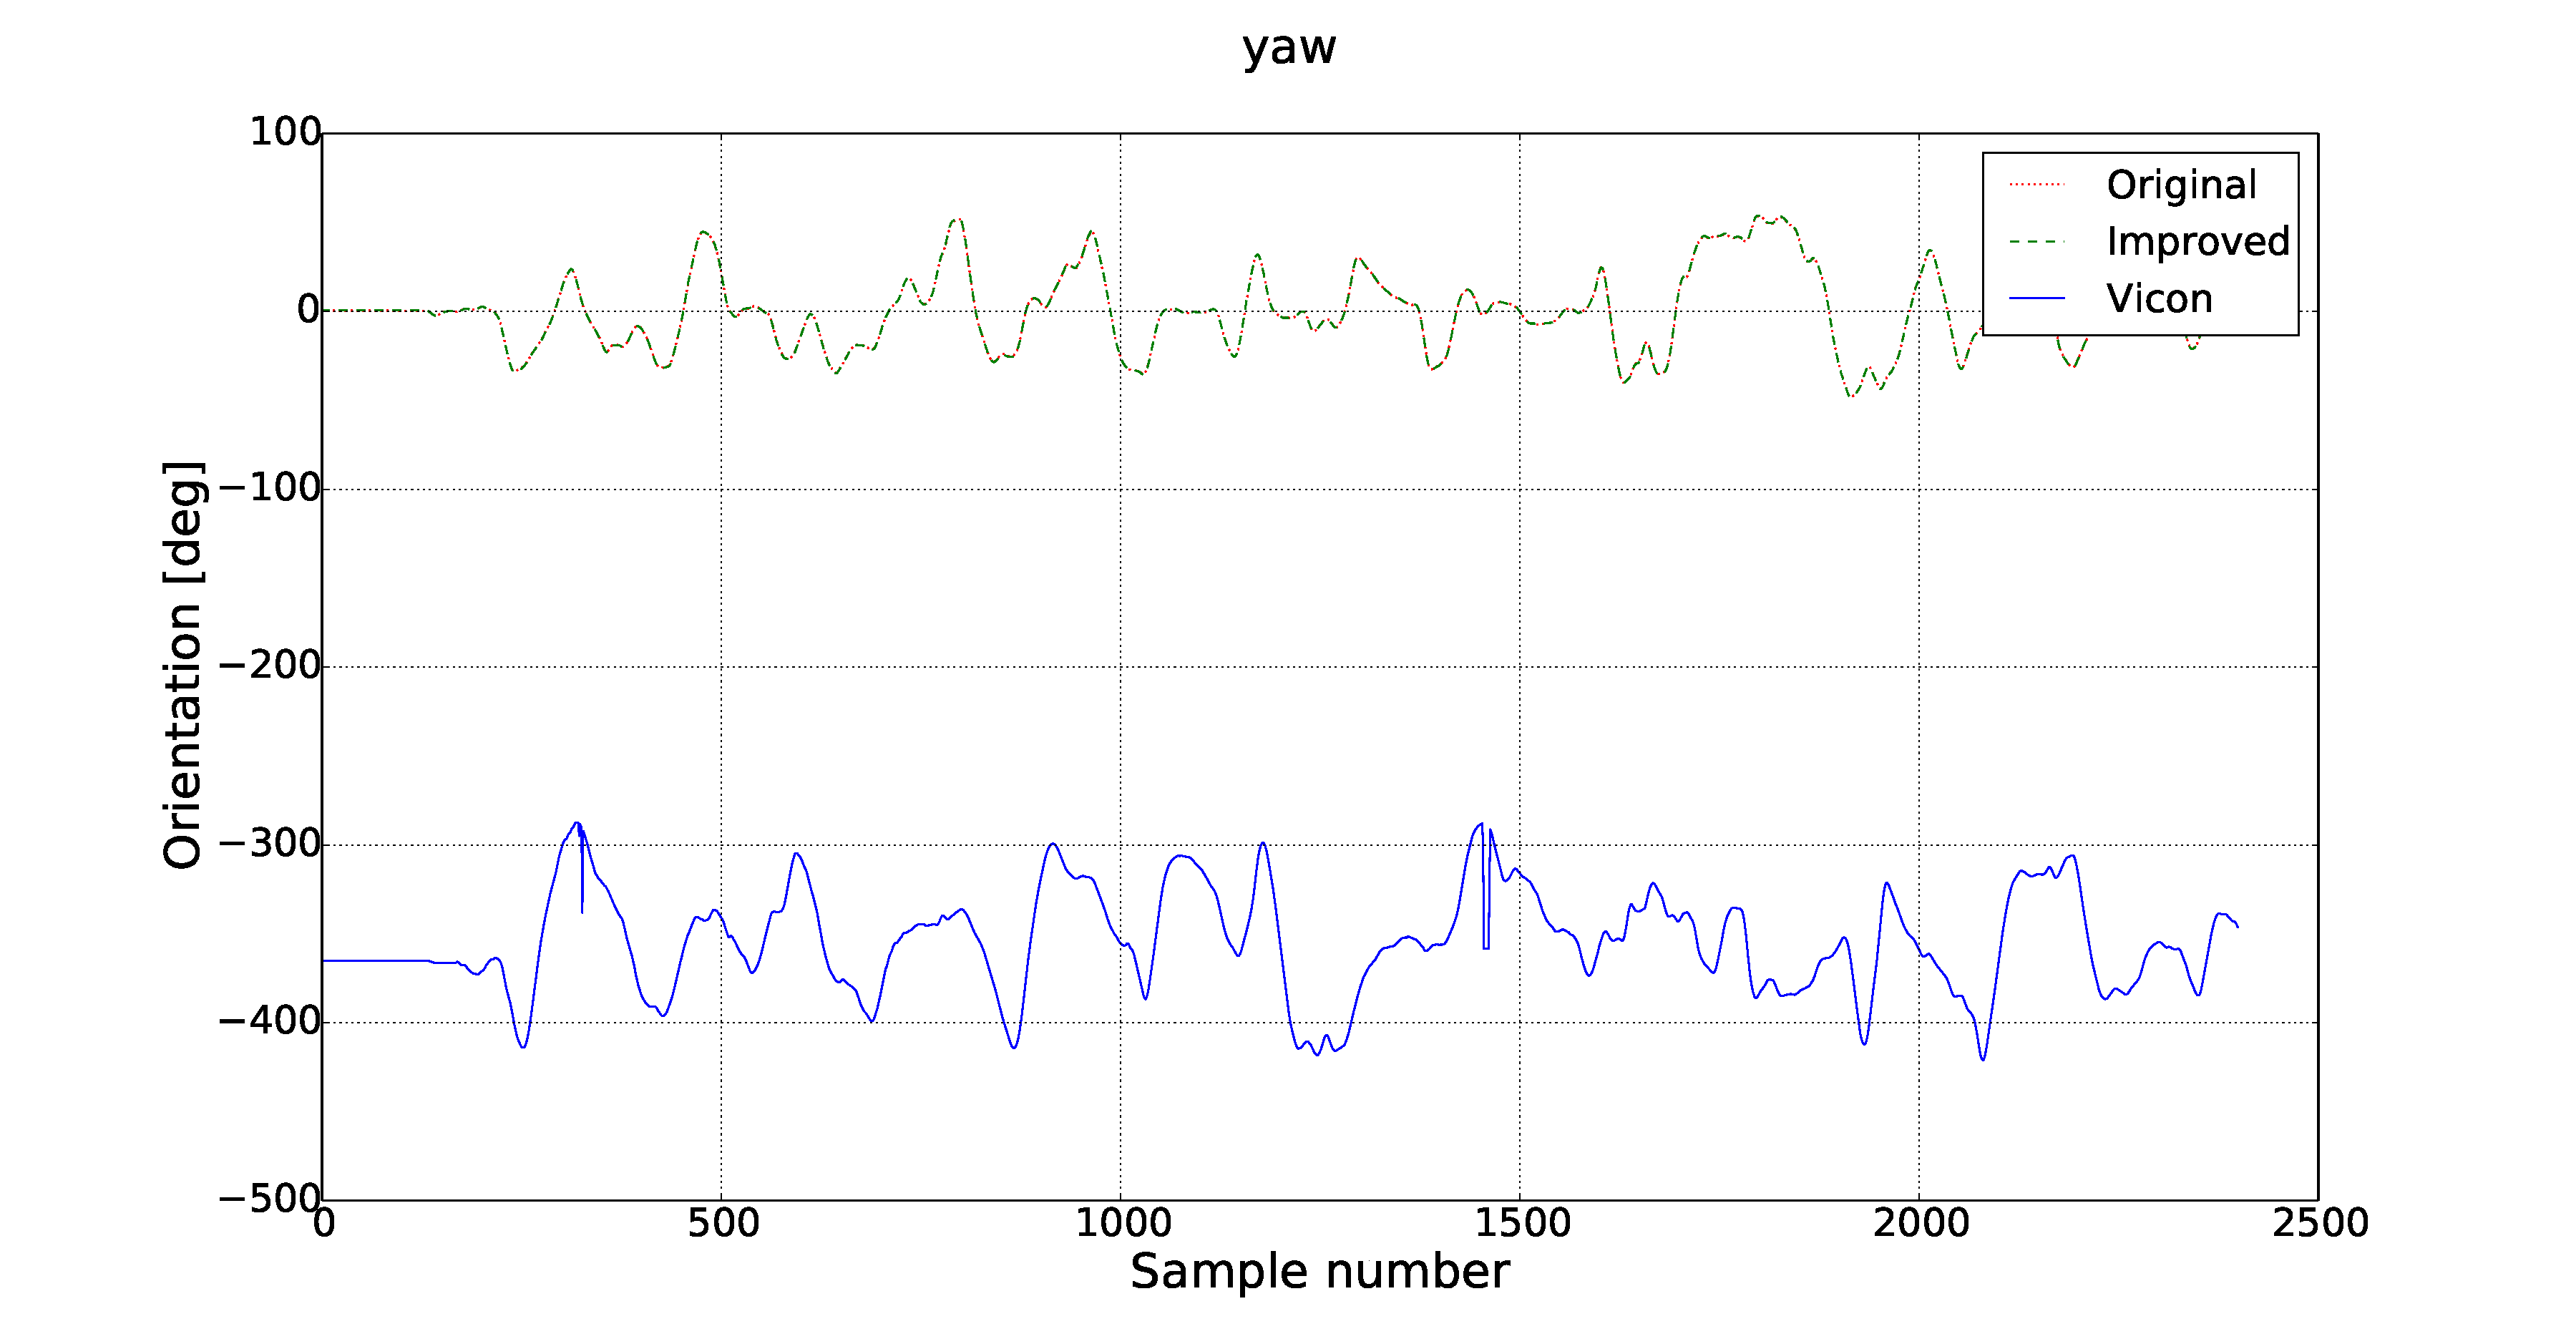
\includegraphics[width=\textwidth]{figures/chapter3/yaw}
    \caption{The ground-truth Vicon pose estimate, versus the original and improved CV pose estimates in the $\psi$ dimension.}
  \label{fig:estimate-yaw}
  \end{subfigure}
  \caption[Plots comparing the Vicon's measurements with the CVS's original and improved measurements. ]{Plots comparing the Vicon's pose measurements with the CVS's original estimate, as well as the estimate with the optimal focal length combination.}
  \label{fig:estimate}
\end{figure*}

It can be seen that there is some improvement in all the dimensions. However, in some cases the improvement in one section of the data set, is negated by worse estimates in another. This can be attributed to the optimisation process, where an improvement at timeframe $t_i$ in the $x$ dimension, for example, may lead to a worse estimate at time $t_i$ in the $\phi$ dimension. However, as the reduction in the two-norm magnitude of the error proves, there is an overall reduction in the error with the optimised data set. It can therefore be concluded that the optimisation procedure did indeed function as expected, producing a focal length combination which led to a more accurate pose estimate from the CVS. 

\subsection{Computer Vision System Accuracy}

Determining the accuracy of a multi-dimensional data model is often a complex task, but since it was found that the error $\bm{\epsilon}$ is normally distributed about zero, it is possible to use the covariance matrix to check the interdimensional variance and dependence. If the off-diagonal elements of the covariance matrix is sufficiently small enough relative to the diagonal elements, it can be deduced that the dimensions are strong enough independent of one another. The covariance matrix $\bm{\Sigma}$ is given in Equation~\ref{eq:covariance-matrix}. 

\begin{equation}
  \label{eq:covariance-matrix}
  \bm{\Sigma} = 
  \begin{bmatrix}
    \bm{3131.7} & 2255.2 & 98.227 & 94.371 &  98.830 & 106.85 \\ 
    2255.2 & \bm{40924}  & 4038.2 & 197.46 &  30.631 & 1953.7 \\
    98.227 & 4038.2 & \bm{5592.5} & 241.75 &  106.86 & 385.23 \\
    94.371 & 197.46 & 241.75 & \bm{84.939} &  10.303 & 13.792 \\
    98.830 & 30.631 & 106.86 & 10.303 &  \bm{110.54} & 63.381 \\
    106.85 & 1953.7 & 385.23 & 13.792 &  63.381 & \bm{318.17} \\
  \end{bmatrix}
\end{equation}

The matrix $\bm{\Sigma}$ shows that there are large off-diagonal elements, indicating that there is strong interdimensional dependence. This dependence is further demonstrated when examining the change in the error in a dimension with respect to the other dimensions. This is demonstrated in the contour plots of Figure~\ref{fig:err-contour}. 

\begin{figure*}
  \centering
  \begin{subfigure}{0.48\textwidth}
    \begin{subfigure}{\textwidth}
      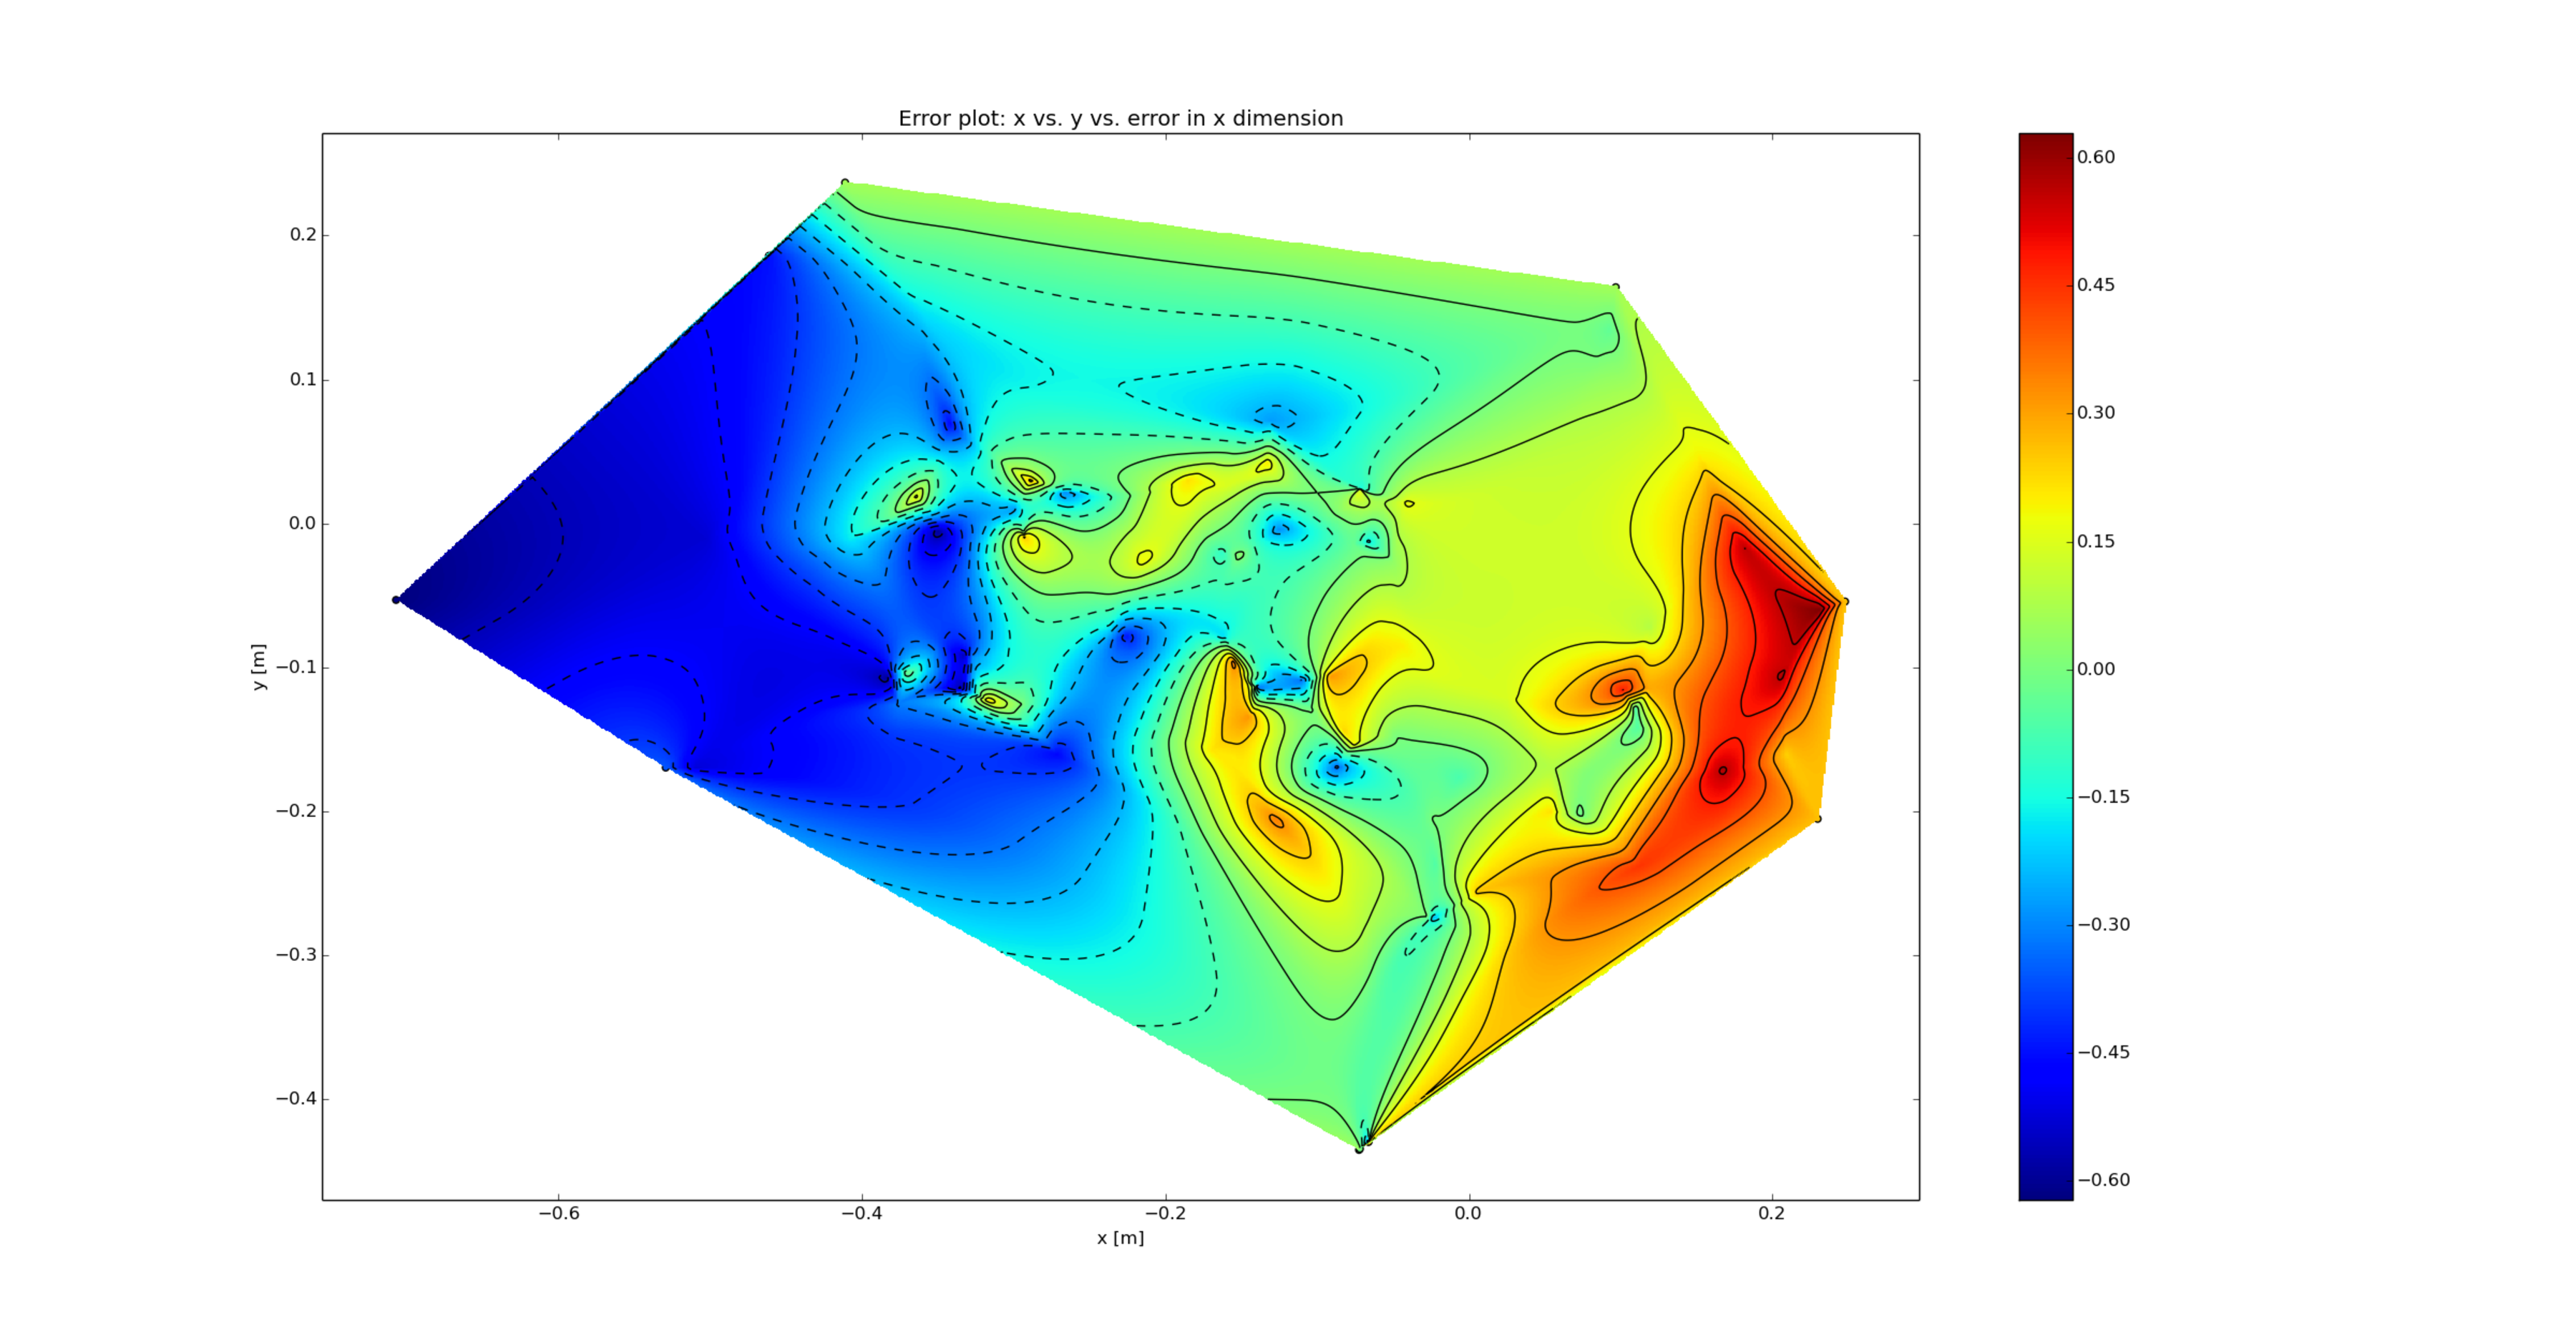
\includegraphics[clip, trim = 120 0 120 0, width=\textwidth]{figures/chapter3/contour_x}
    \end{subfigure}
    \begin{subfigure}{\textwidth}
      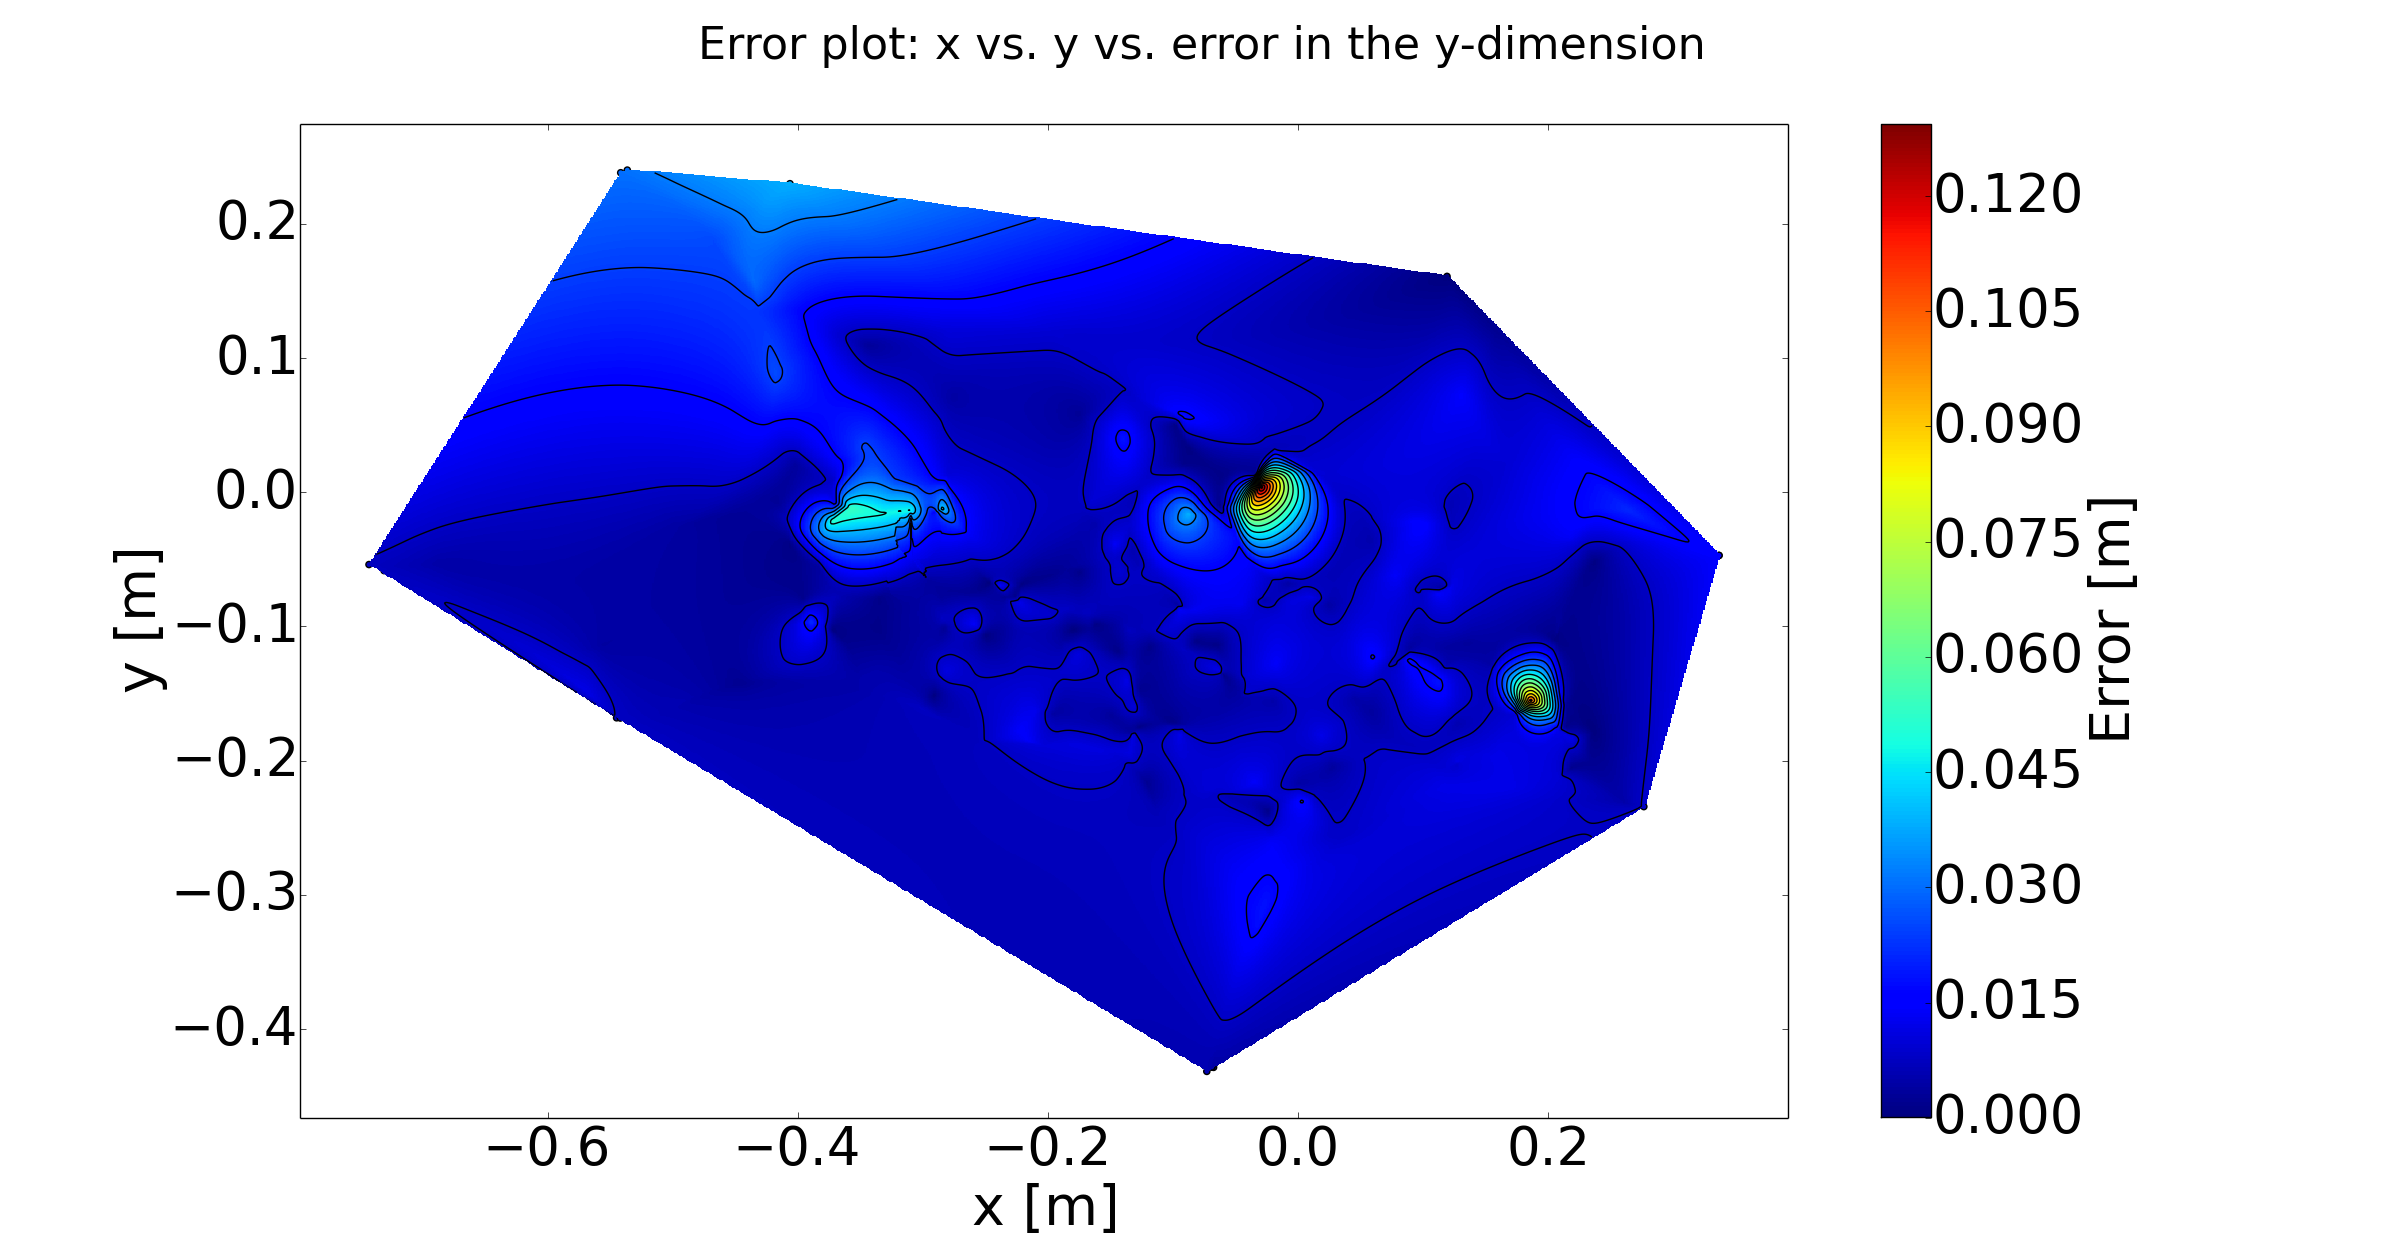
\includegraphics[clip, trim = 120 0 120 0, width=\textwidth]{figures/chapter3/contour_y}
    \end{subfigure}
    \begin{subfigure}{\textwidth}
      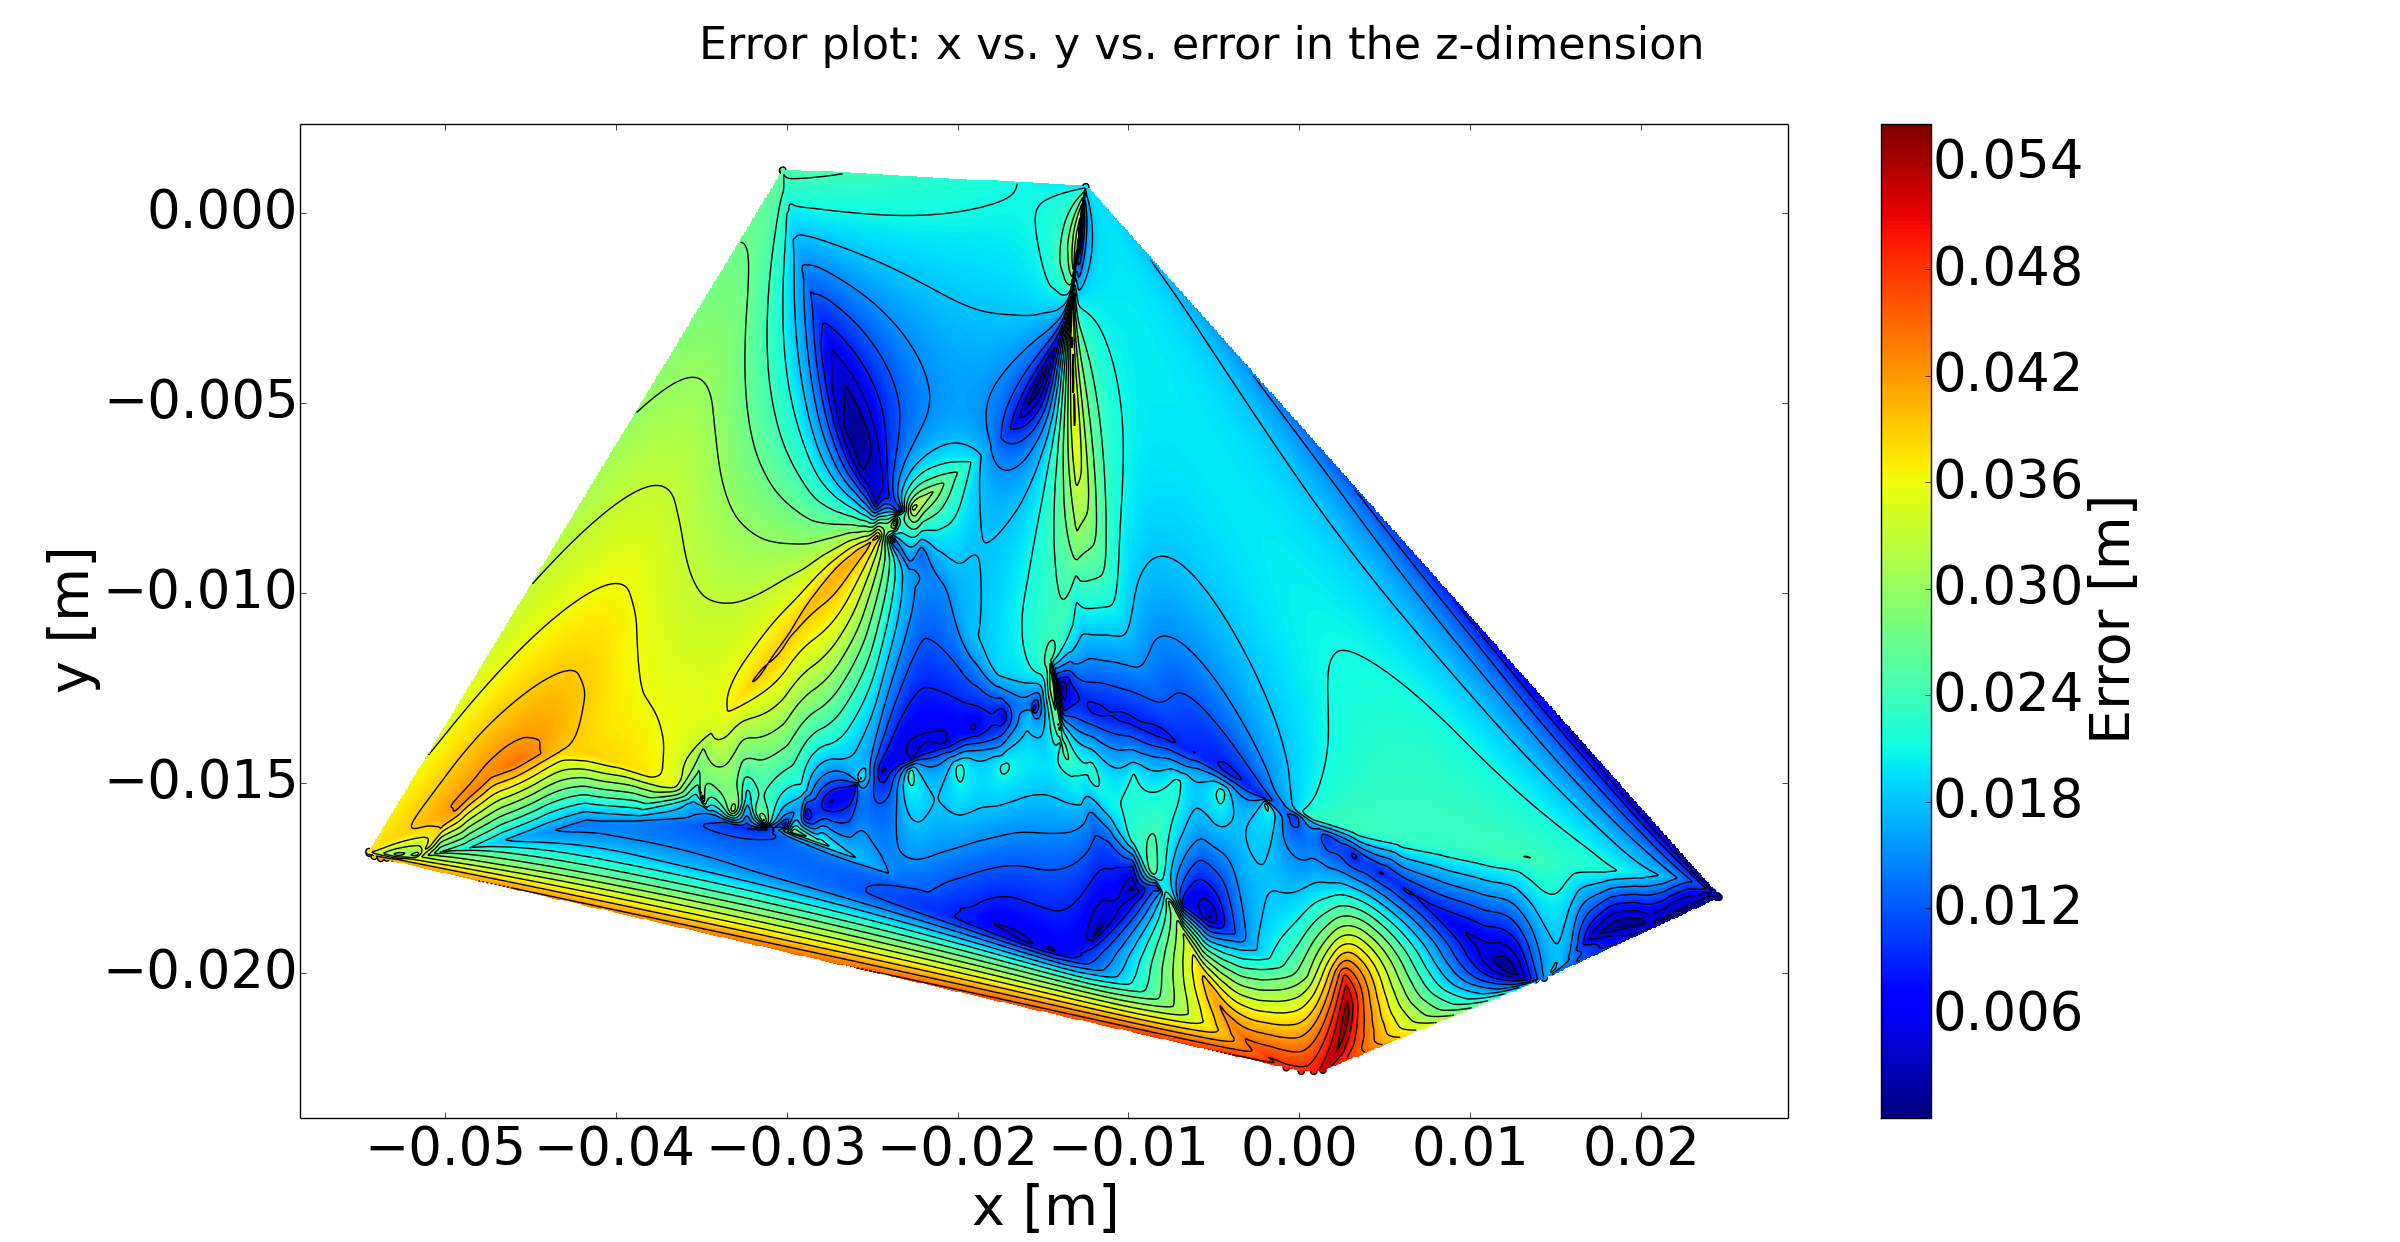
\includegraphics[clip, trim = 120 0 120 0, width=\textwidth]{figures/chapter3/contour_z}
    \end{subfigure}
    \caption{Error contour plots for the position dimensions. Units in m.}
  \end{subfigure}
  ~
  \begin{subfigure}{0.48\textwidth}
    \begin{subfigure}{\textwidth}
      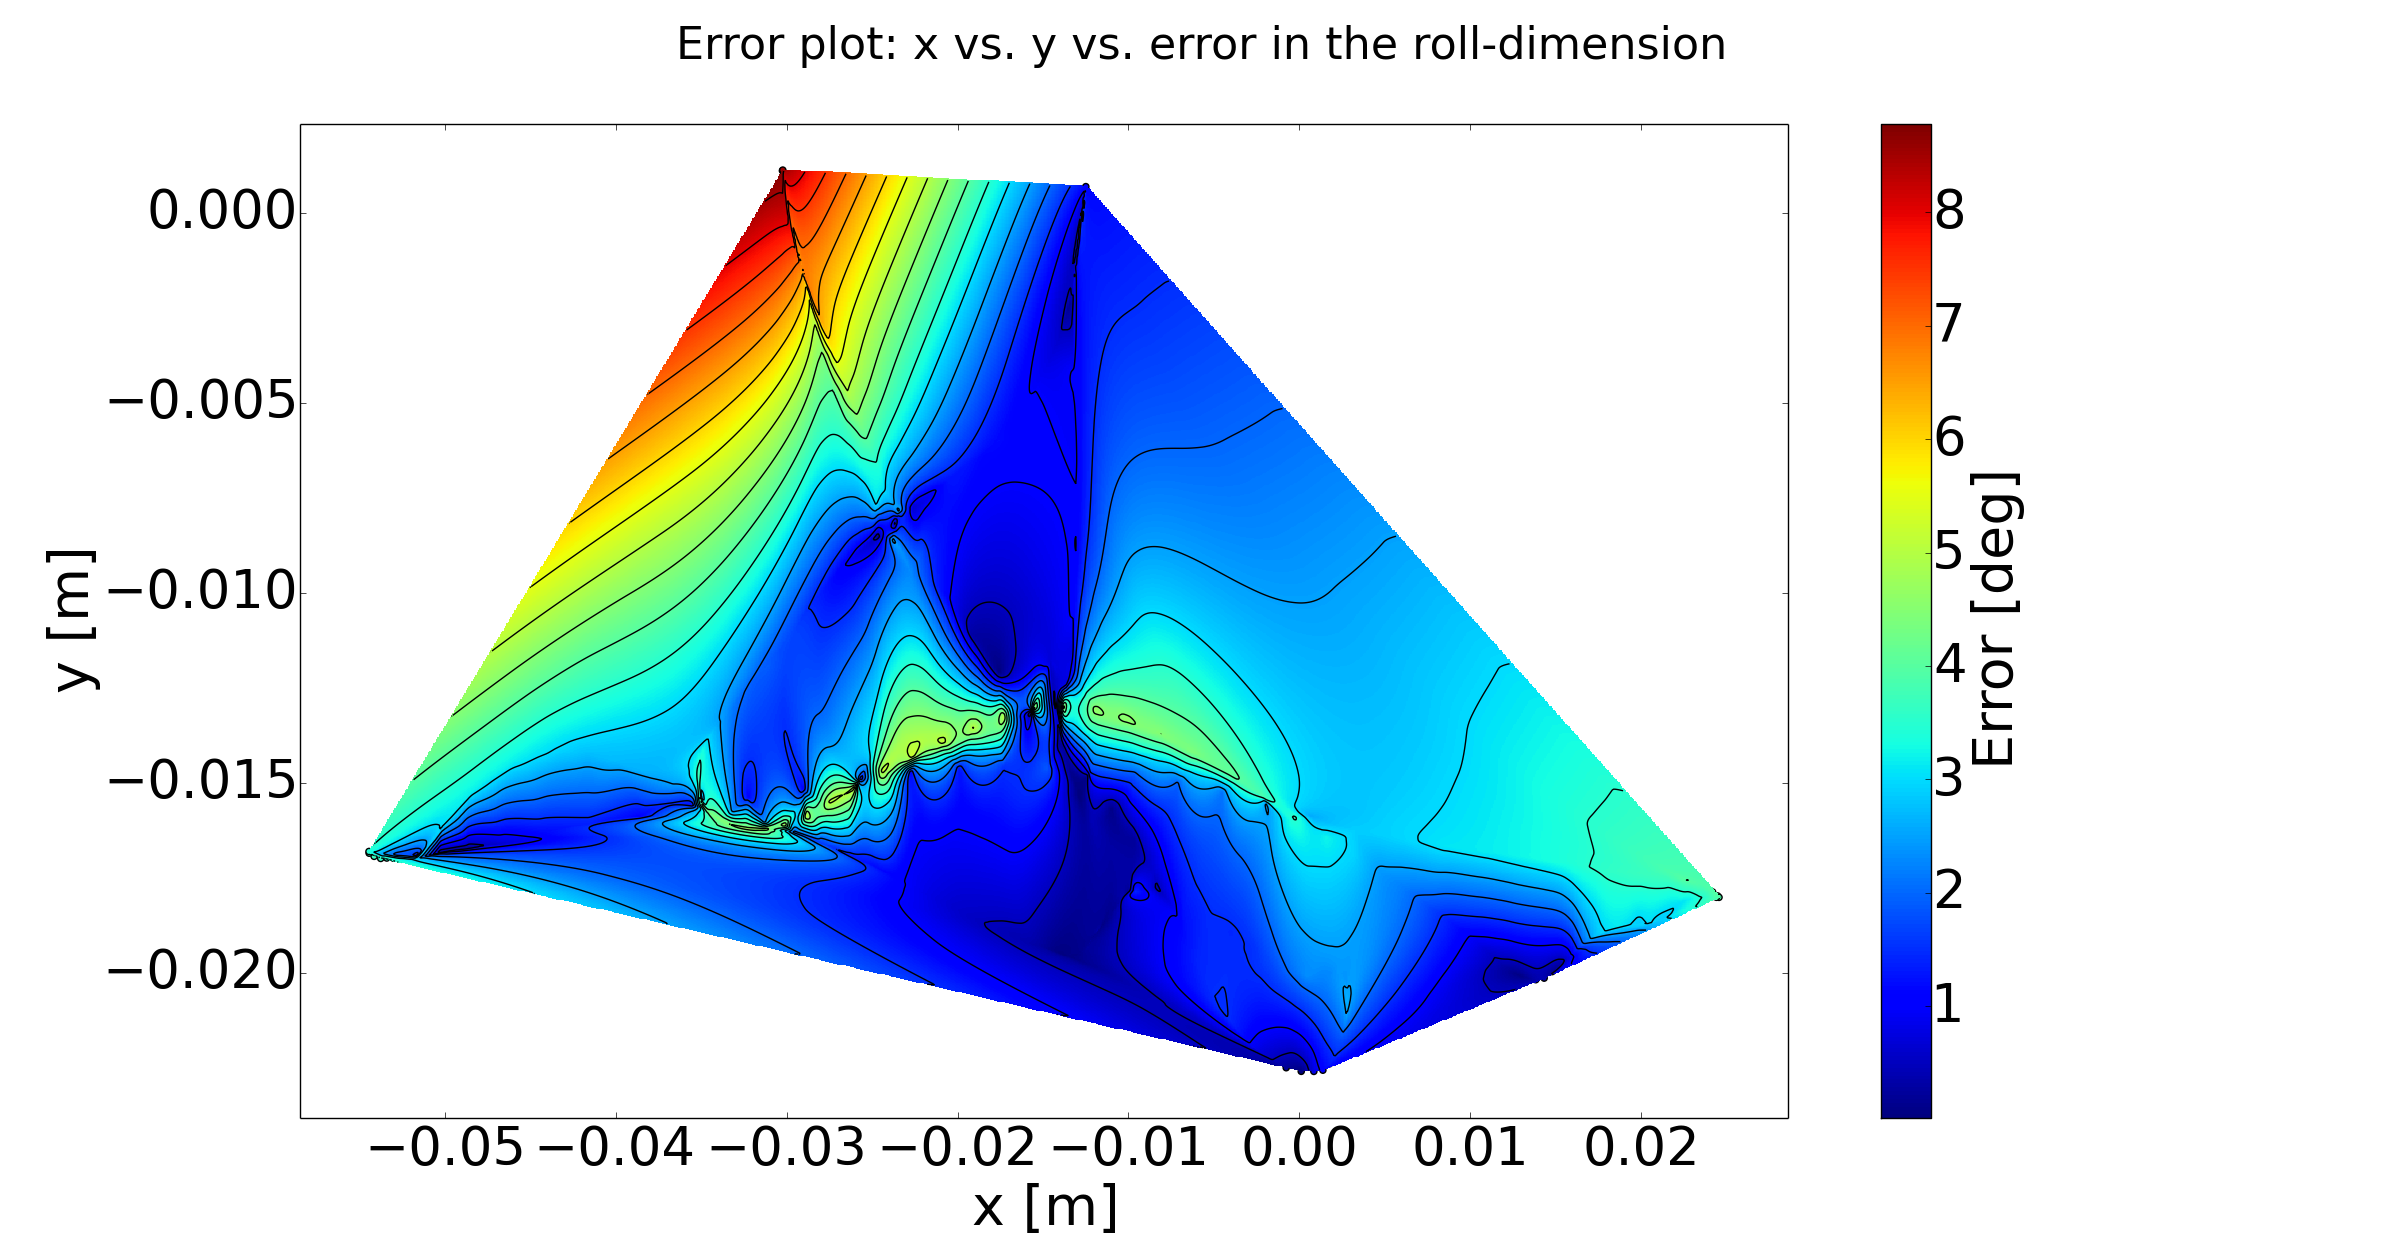
\includegraphics[clip, trim = 120 0 120 0, width=\textwidth]{figures/chapter3/contour_roll}
    \end{subfigure}
    \begin{subfigure}{\textwidth}
      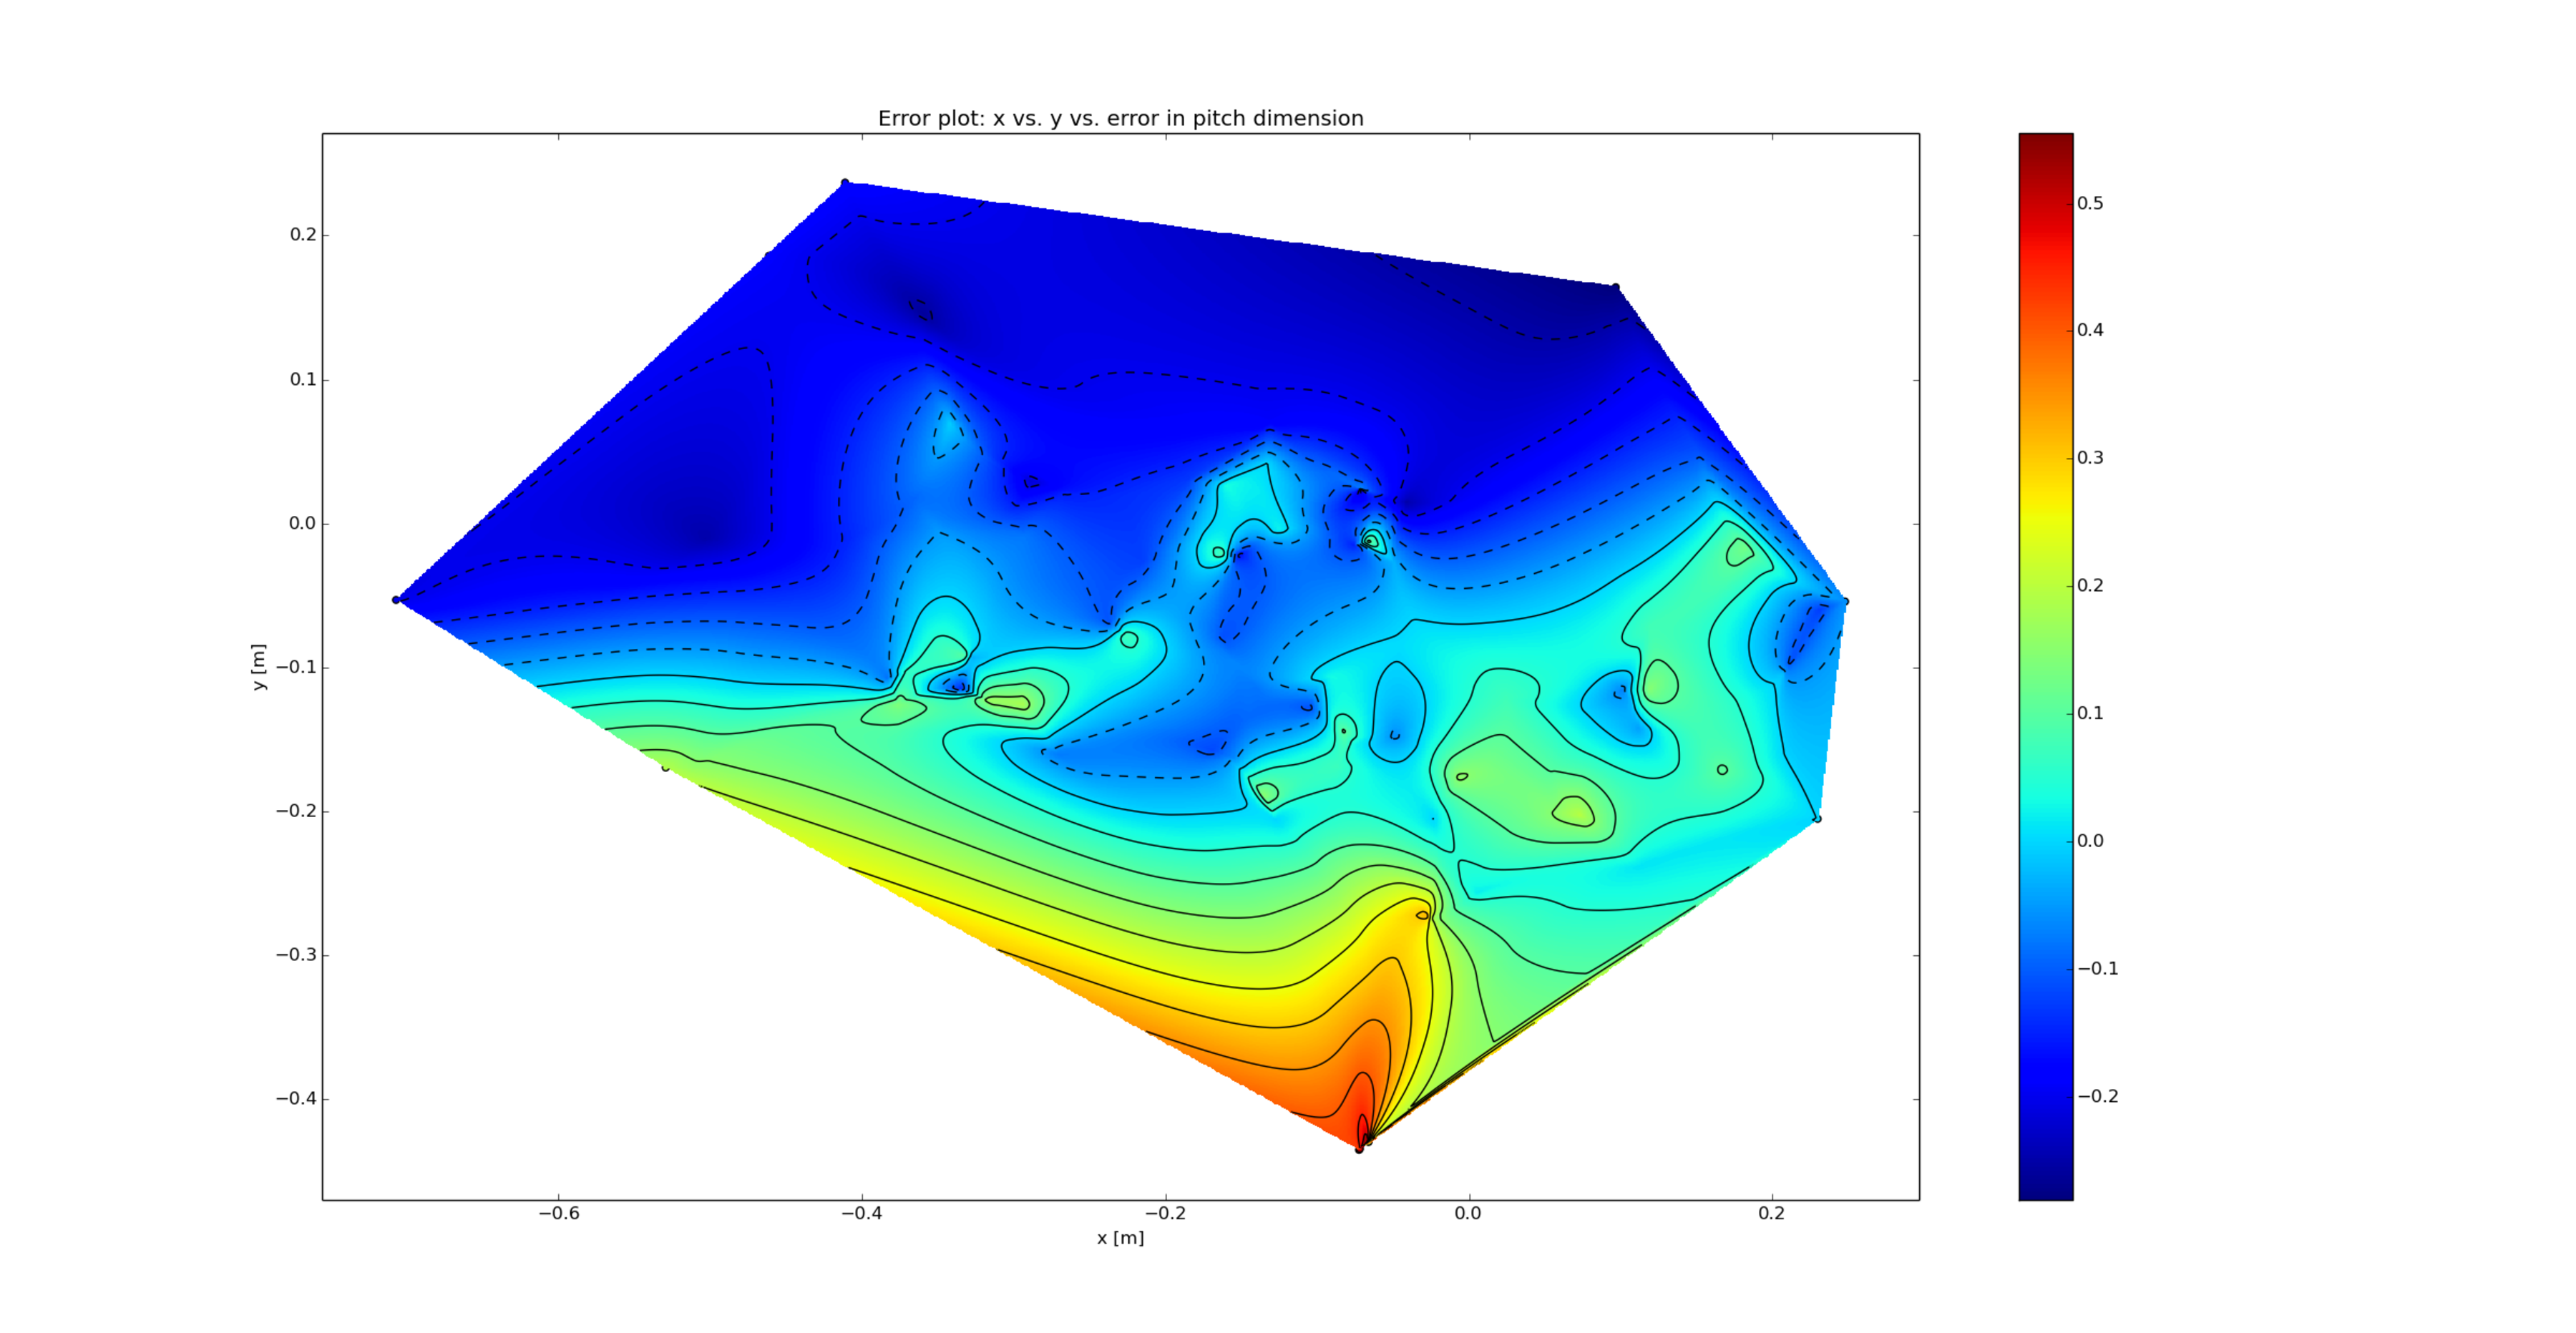
\includegraphics[clip, trim = 120 0 120 0, width=\textwidth]{figures/chapter3/contour_pitch}
    \end{subfigure}
    \begin{subfigure}{\textwidth}
      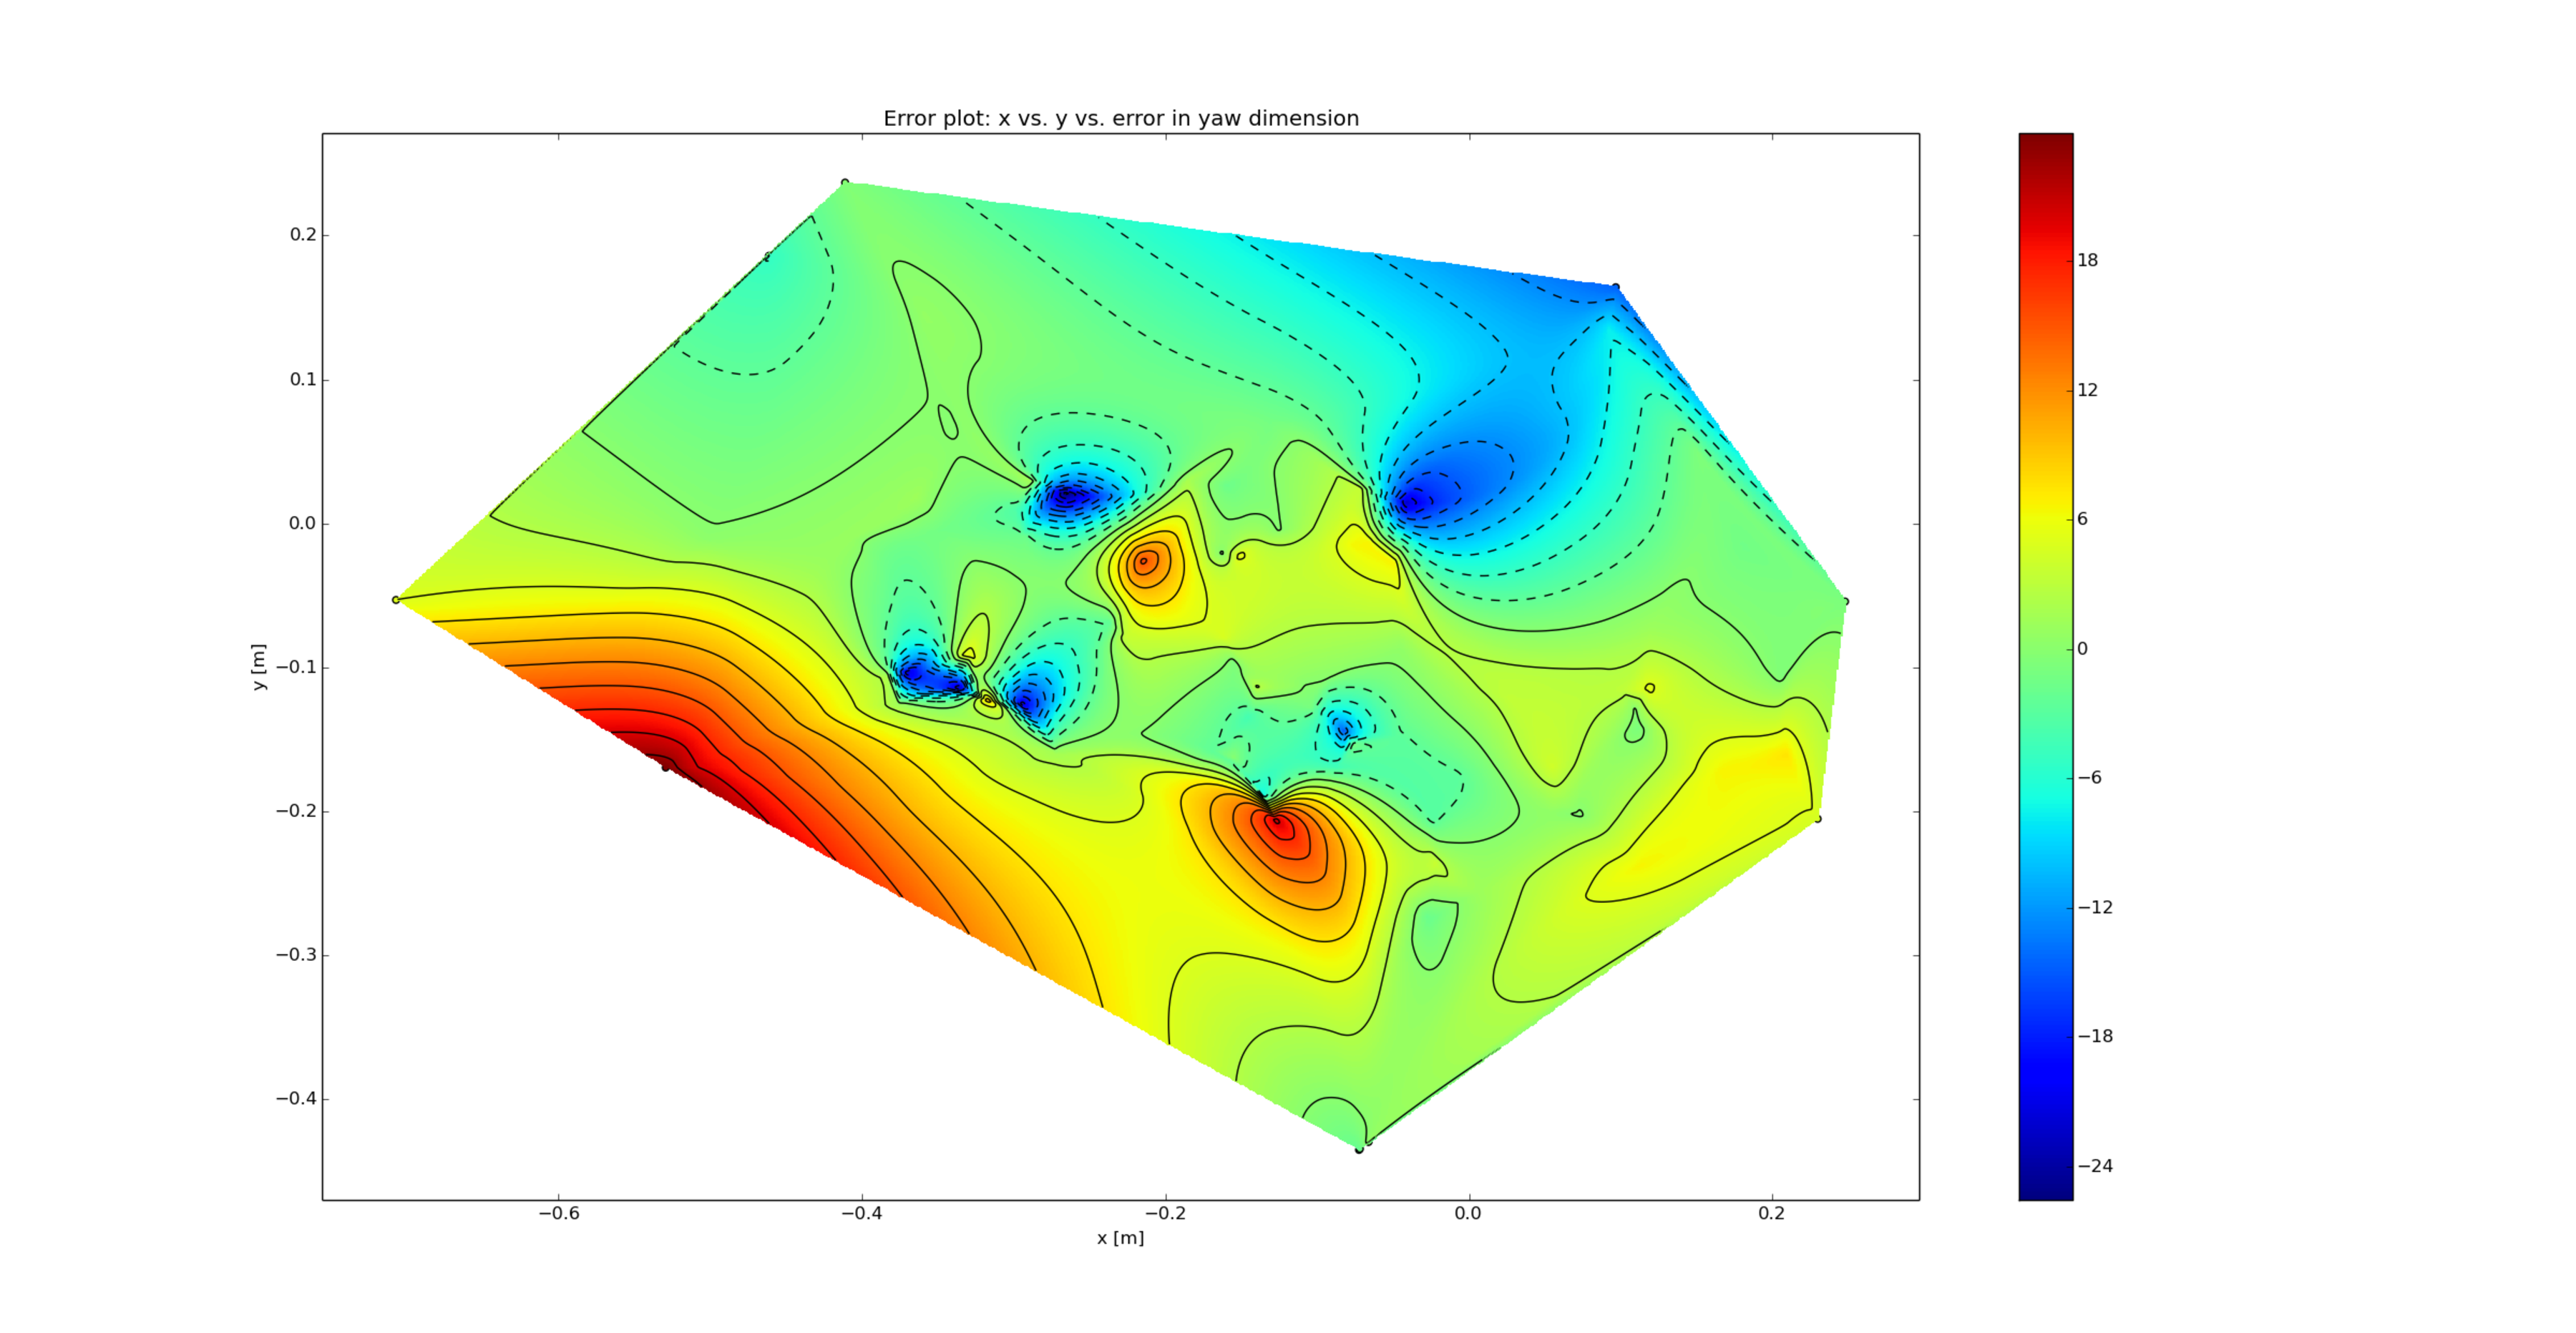
\includegraphics[clip, trim = 120 0 120 0, width=\textwidth]{figures/chapter3/contour_yaw}
    \end{subfigure}
    \caption{Error contour plots for the orientation dimensions. Units in \textdegree.}
  \end{subfigure}
  \caption[A collection of contour plots of the position and orientation vectors relative to one another]{A collection of contour plots of the position and orientation vectors relative to one another.}
  \label{fig:err-contour}
\end{figure*}

From Figure~\ref{fig:err-contour} it can be seen that the error in a dimension varies when the two other pose dimensions changes. 

These plots, as well as the covariance matrix $\bm{\Sigma}$ indicates that there is no clear indication on the accuracy of the CVS, since its a function of the pose of the calibration board relative to the CVS's camera. 

\section{Conclusion}

In this chapter, the design and layout of a computer vision measurement system (CVS) was discussed. The system consists of hardware and software components and the details of both were discussed. The system was tested in an indoor measurement facility to determine its measurement accuracy. With the ground-truth measurements produced by this indoor system, it was possible to optimise the intrinsic camera parameters and improve the pose data from the CVS.

It was shown that the error data is a function of the pose of the calibration board relative to the CVS's camera. This constant error variation makes difficult to determine the measurement accuracy of a sample pose vector from the CVS.\@ The measurement accuracy of the CVS is very important and cannot be ignored. Therefore, another approach to determine the measurement accuracy was taken and was investigated. 

%\chapter{Pose Error Estimation}

\section{Introduction}

The main objective of this project is to determine a quadcopter's the pose estimation accuracy, with its pose given by its on-board sensors. Here, the pose refers to a six-dimensional vector describing an object's position and angular orientation. The pose estimation accuracy must be performed in the outdoors to allow the quadcopter to use its global positioning sensor (GPS). To this end, a computer vision pose measurement system (CVS), which extracts six-dimensional pose data from a calibration object in the system's view, was designed and implemented. Before the CVS was used to make pose measurements, its measurement accuracy was first determined. 

In Chapter meme it was found that the pose measurement error of the CVS has high interdimensional dependence, as demonstrated by the covariance matrix of the error and the contour plots in Figure meme, and, despite using the RANSAC algorithm to filter out any outlier data points, the data is still fairly complex and noisy. This means that the measurement error is constantly changing and varies with the calibration board's current pose relative to the CVS's camera.

In the context of this project, it is important to know what the accuracy of a pose measurement sample is to ensure that it is more accurate than the pose estimate from the quadcopter. This makes it necessary to be able to determine the measurement error of any arbitrary pose measurement sample of the CVS.\@ It was decided that machine learning method will be employed to accomplish this. Machine learning is where a computer model is trained to recognise patterns within a set of input data and output information on the patterns which are of interest to the model's designer. 

This chapter sets out to explain the process behind making a machine learning model that can estimate, within reasonable accuracy, what the pose measurement error of the CVS is for any arbitrary input measurement vector. 

\section{Model Design}

\subsection{Background}

Designing a machine learning model can consist of three basic steps. These steps are listed as follows:

\begin{enumerate}
  \item Select machine learning model type.
  \item Train the model.
  \item Validate the model's accuracy. 
\end{enumerate}

First, the model type is selected. As stated previously, the CVS's pose measurement data is fairly complex, interdimensionally dependant and is high dimensional. A neural network model was therefore selected as a basis. It has been shown by~\cite{tu1996advantages} that neural networks excel at handling complex data and detecting and extracting complex non-linear relationships within the input data. Furthermore, the radial basis neural network (RBFNN) was chosen as a neural network topology. RBFNN's provide superior results, when compared to traditional feed-forward networks, when noisy data sets are used, as proven by~\cite{xie2011comparison}. The data is not time dependant, making the recurrent neural network topology unnecessarily complex for this application.  

Next, model training takes place. Here, the network is trained to take an input and adjust is internal weights in such a way that the input data is best related to a desired output by using a supervised training scheme, such as the backpropagation procedure. In this case, the network input would be the six-dimensional pose vector produced by the CVS and the network output is the corresponding measurement error of the input pose vectors.  

Finally, to test and validate the accuracy of the trained model, it is tested with another set of input pose data of which the measurement error is already known. These two data sets can be used to select and refine the training parameters of the model. 

The design process is iterative, where steps 2 and 3, and perhaps 1, can be repeated until a model which outputs satisfactory results is produced. 

\subsection{Model Training}

Training a machine learning model is perhaps the most crucial aspect of the model design phase. Here the hidden layer of the RBFNN's nodes are initialised and assigned a weighting factor. This weight is selected in such a way that it minimises the difference between the network's output and the training error data by using the backpropagation method, demonstrated in Figure~\ref{fig:chap4-backprogagation}.

\begin{figure}
  \centering
  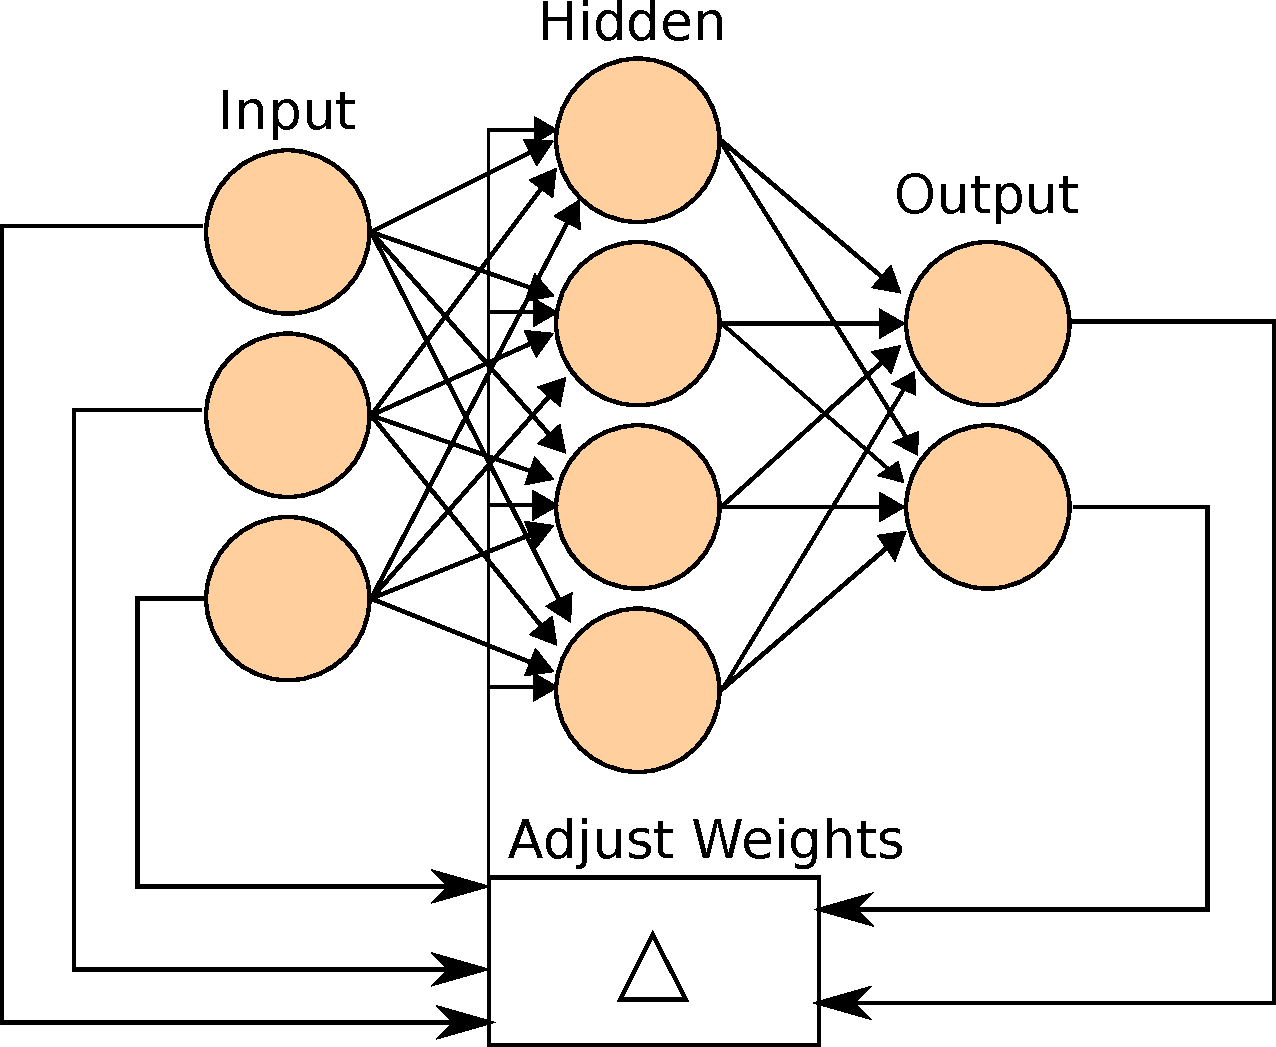
\includegraphics[width=0.5\textwidth]{figures/chapter4/backpropagation}
  \caption[A neural network implementing the backpropagation procedure.]{A figure of a neural network implementing the backpropagation procedure. Adopted from~\cite{ann-wiki-pic}.}
\label{fig:chap4-backprogagation}
\end{figure}

The backpropagation method works as follows. The hidden nodes are initialised with a weighting factor. The input training data is then fed to the network and the output is compared to the training set's output data. Based on this difference, the different nodes' weighting factors are adjusted. Then, the input data is fed to the adjusted network again and the new output is compared to the output training data. This process is repeated until the mean square error of the output's deviation from the training data falls below a set threshold. 

Factors that will affect the network's accuracy are the number of nodes in the hidden layer, as well as the strictness of fit. The number of hidden nodes is a measure of the complexity of the network and reflects the complexity of the data it can process. However, when too many nodes are selected, there is a significant risk that the model will only capture and attempt to model the noise and outlier data in a data set, instead of characterising the underlying relationships between the input and output. This phenomenon is known as overfitting and can be observed when a model with a very small training error is exposed to new input data and the error is a few orders of magnitude larger than for the training data. Here, the model describes the training data set very well, but any data set that is not very similar to the training data set will be handled very poorly. This is why the model validation phase is a very important aspect of model training, to ensure that overfitting does not take place. 

To train the model for this project, two sets of data were used, one for training and another for the model validation. Both of these data sets were taken from the data sets generated during the Vicon measurement test, where the measurement accuracy of the CVS was determined by comparing its measurements to that of the measurements made by a Vicon system. It includes both the pose data from the CVS and the corresponding measurement error. It was decided to use 300 training samples, giving 50 samples per dimension. The input and output training data sets were normalised to a range of $[-1, 1]$, since the pose vector contains different measurement units (degrees and metres). All subsequent inputs to and outputs from the network must be normalised and denormalised with the same values that the training data was normalised with.  

Matlab's\footnote{Matlab v8.4.0.150421 (R2014)} Neural Network toolbox\footnote{Neural Network Toolbox v8.2.1} was used to train the RBFNN and get the output for subsequent input data. The function prototype is given by 

\begin{center}
  \verb|net = newrb(P,T,goal,spread,MN,DF)|
\end{center}

Here, $P$ and $T$ are the $300\times6$ input and output training data matrices. The `goal' parameter is the error threshold for the training data and `spread' is the strictness of fit parameter, while $MN$ and $DF$ define the maximum number of hidden nodes and dictate the amount of nodes to increase by between each training iteration. Adjusting the `spread' and $MN$ parameters are the primary ways of adjusting the network's accuracy and output. 

\subsection{Model Validation}

The model validation phase is used to ensure that the RBFNN has been properly trained and that overfitting does not occur. The validation data set comes from the same Vicon test the training data comes from. Another 300 pose measurement samples were used for the validation data set. 

The error was determined by feeding the validation input data into the trained network and comparing its output with the validation error data. The mean square error was used as a measure of accuracy. 

\section{Results}

With the training and validation data sets selected, the model design could begin. Different combinations of training parameters for the `newrb' Matlab function were tested. It was found that the `spread' parameter played the largest part in the mean square error during training. This is because the training data changes relatively quickly and contains a fair amount of noise. It was found that forcing the RBFNN to go through all the points caused the mean square error to go up when it was tested with the validation set. It was therefore decided to keep the spread parameter small to allow the RBFNN to describe the general trend in the data. 

Furthermore, changing the maximum number of nodes also influenced the accuracy of the network. Leaving the $MN$ parameter to its default will let the maximum number of hidden nodes go up to the number of training samples, i.e.\ 300 nodes in this case. This makes the network overly complex and slow. It was found that the network performs better with both the training and validation data sets with a lower number of nodes, at about 10\% of the number of samples. 

A combination that was found to work well, was a `spread' of 1\e{-3} and 20 hidden nodes. This combination gives a mean square error of approximately 3.0, whereas the default values of 1 and 300 gives a mean square error of 5\e{3} meme bewys, indicating a significant improvement in accuracy. SIT IN TRAINING AND VALIDATION GRAFIEKE. BESPREEK AKKURAATHEID VAN AFSKATTINGS.  

Figure~\ref{fig:chap4-rbf-train} shows results of the RBFNN model when tested with the training data set. It can be seen that the model's estimate very closely resembles the training set's error, indicating that the model is well-trained. 

\begin{figure*}
  \begin{subfigure}{0.3\textwidth}
    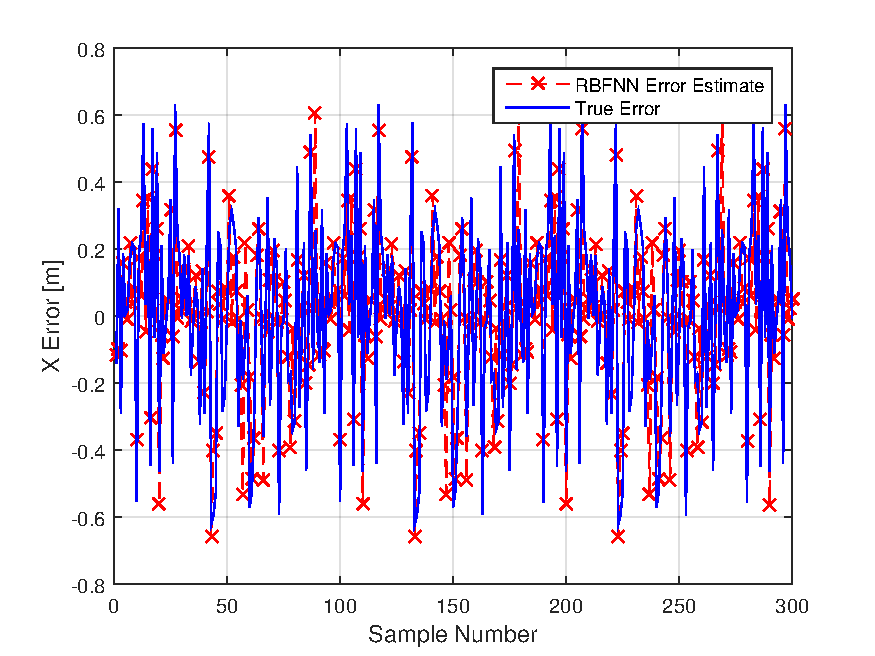
\includegraphics[width=\textwidth]{figures/chapter4/x_train}
    \caption{}
  \end{subfigure}
~
  \begin{subfigure}{0.3\textwidth}
    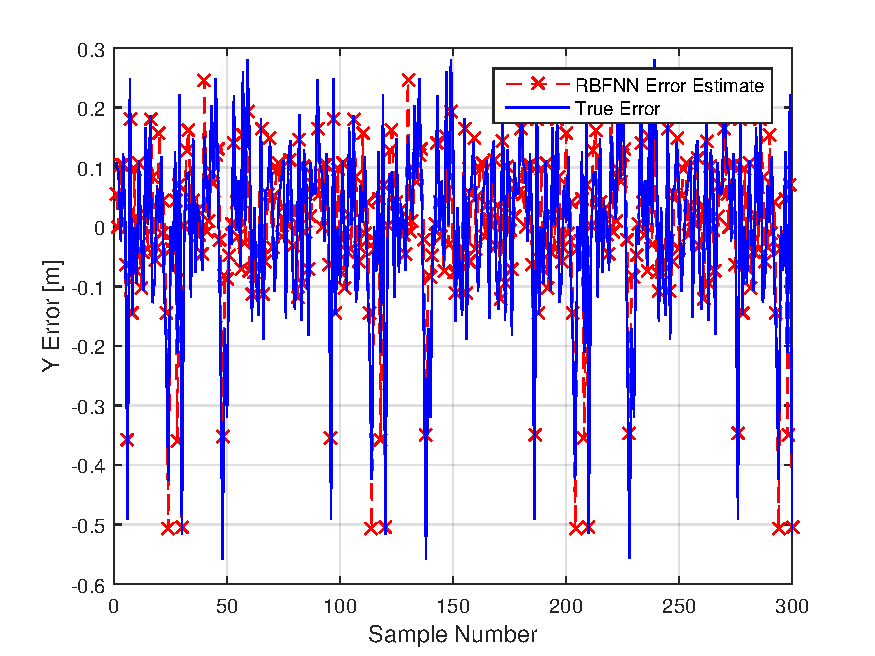
\includegraphics[width=\textwidth]{figures/chapter4/y_train}
    \caption{}
  \end{subfigure}
~
  \begin{subfigure}{0.3\textwidth}
    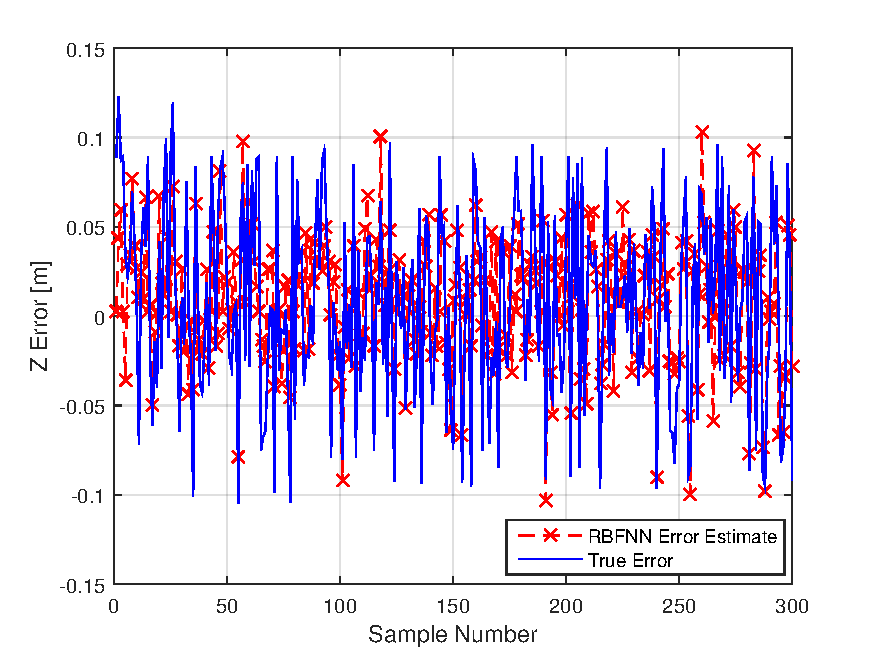
\includegraphics[width=\textwidth]{figures/chapter4/z_train}
    \caption{}
  \end{subfigure}
~
  \begin{subfigure}{0.3\textwidth}
    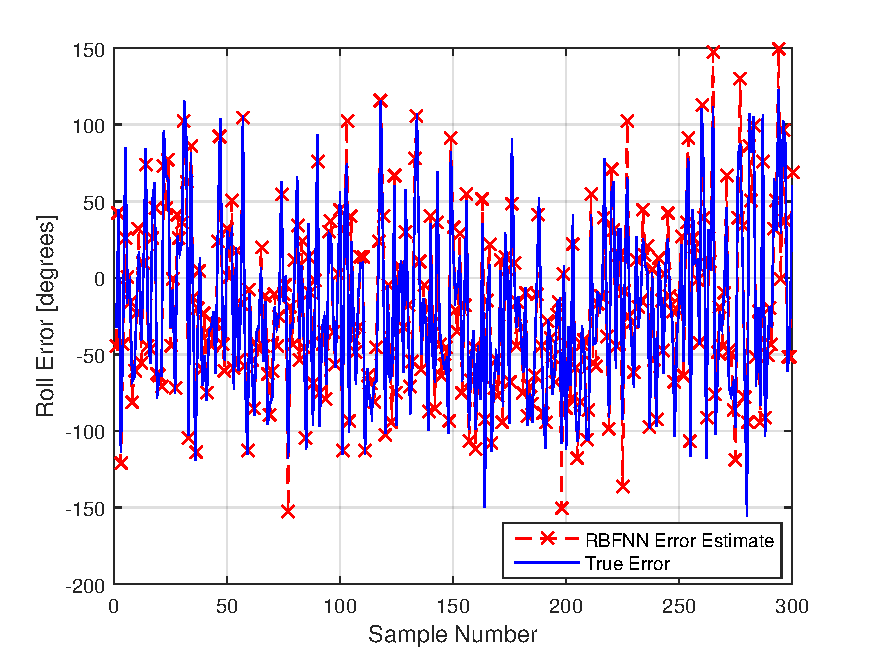
\includegraphics[width=\textwidth]{figures/chapter4/roll_train}
    \caption{}
  \end{subfigure}
~
  \begin{subfigure}{0.3\textwidth}
    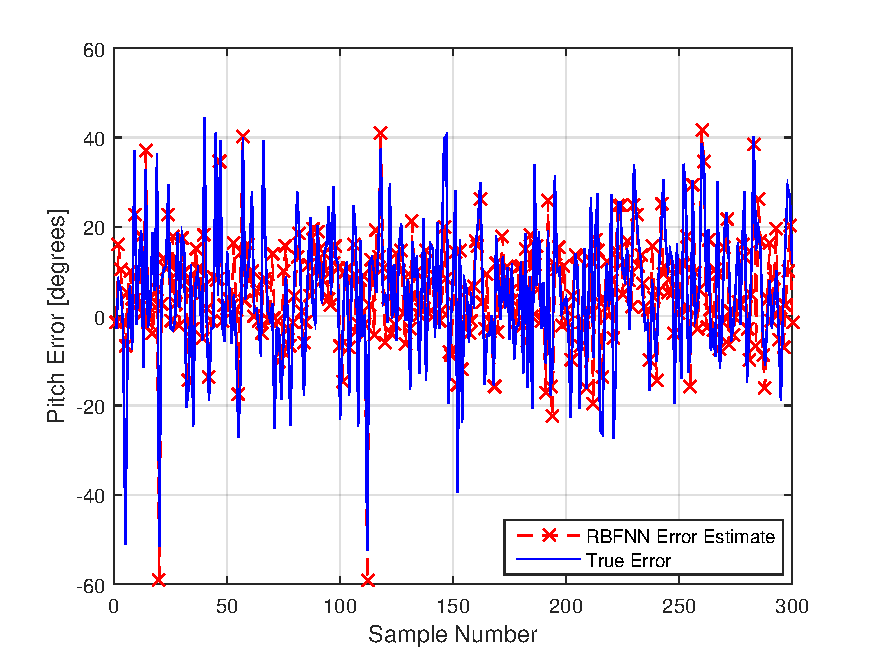
\includegraphics[width=\textwidth]{figures/chapter4/pitch_train}
    \caption{}
  \end{subfigure}
~
  \begin{subfigure}{0.3\textwidth}
    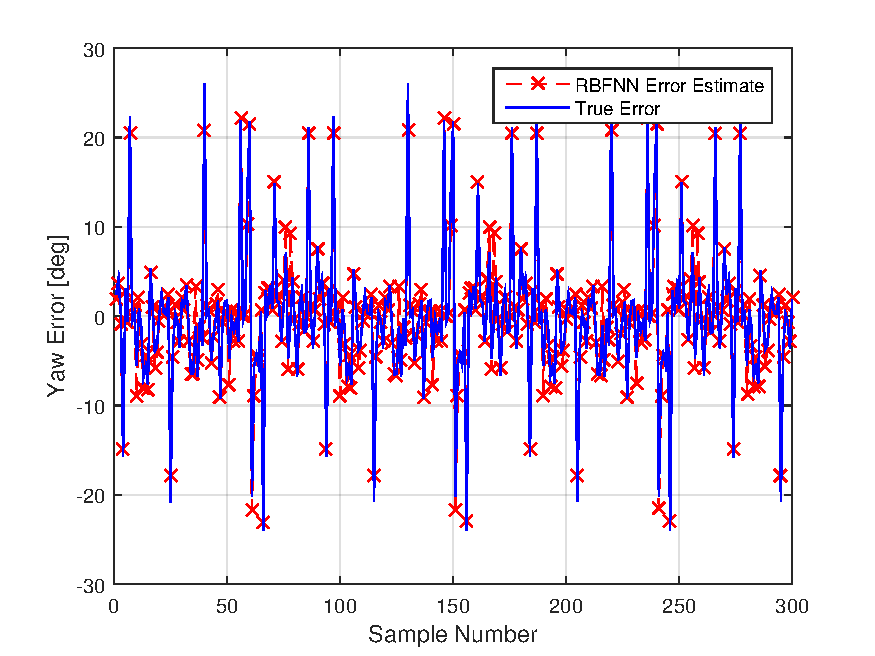
\includegraphics[width=\textwidth]{figures/chapter4/yaw_train}
    \caption{}
  \end{subfigure}
  \caption[The output of the RBFNN when used with the training set input.]{A plot of the output of the RBFNN for the different dimensions when used with the training data set.}
  \label{fig:chap4-rbf-train}
\end{figure*}

Figure~\ref{fig:chap4-rbf-valid} shows the model's output when tested with the validation data set.

\begin{figure*}
  \begin{subfigure}{0.3\textwidth}
    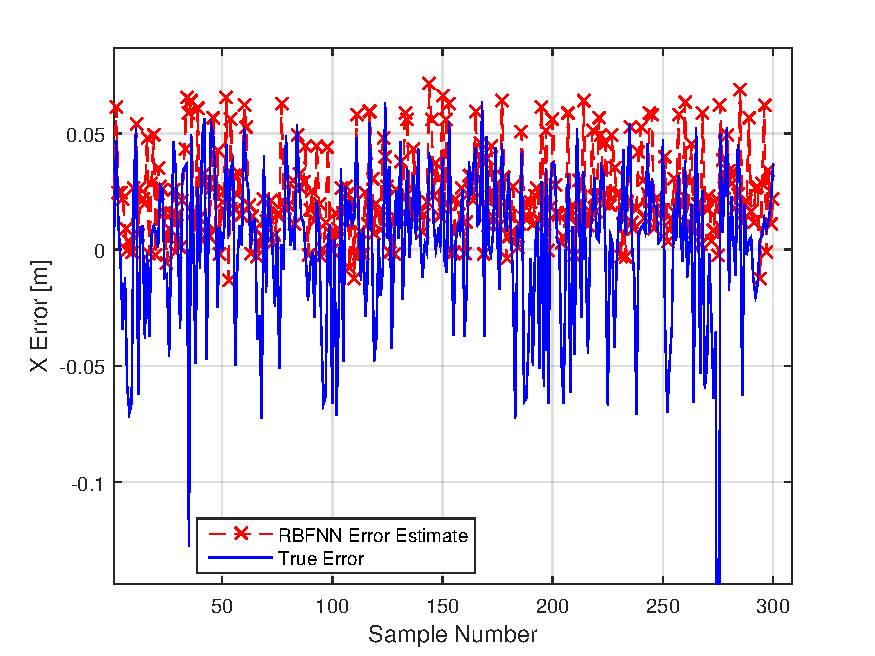
\includegraphics[width=\textwidth]{figures/chapter4/x_valid}
    \caption{}
  \end{subfigure}
~
  \begin{subfigure}{0.3\textwidth}
    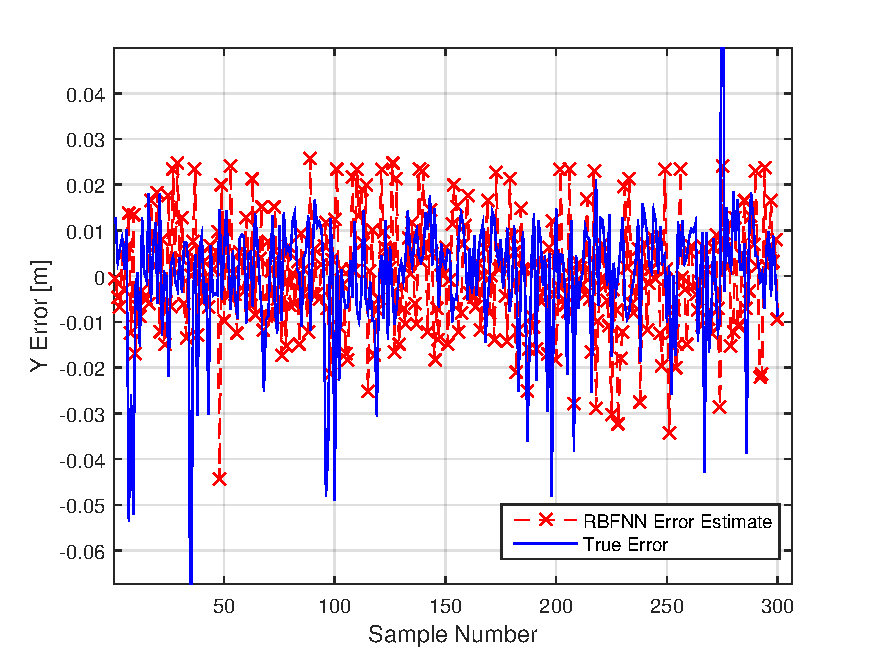
\includegraphics[width=\textwidth]{figures/chapter4/y_valid}
    \caption{}
  \end{subfigure}
~
  \begin{subfigure}{0.3\textwidth}
    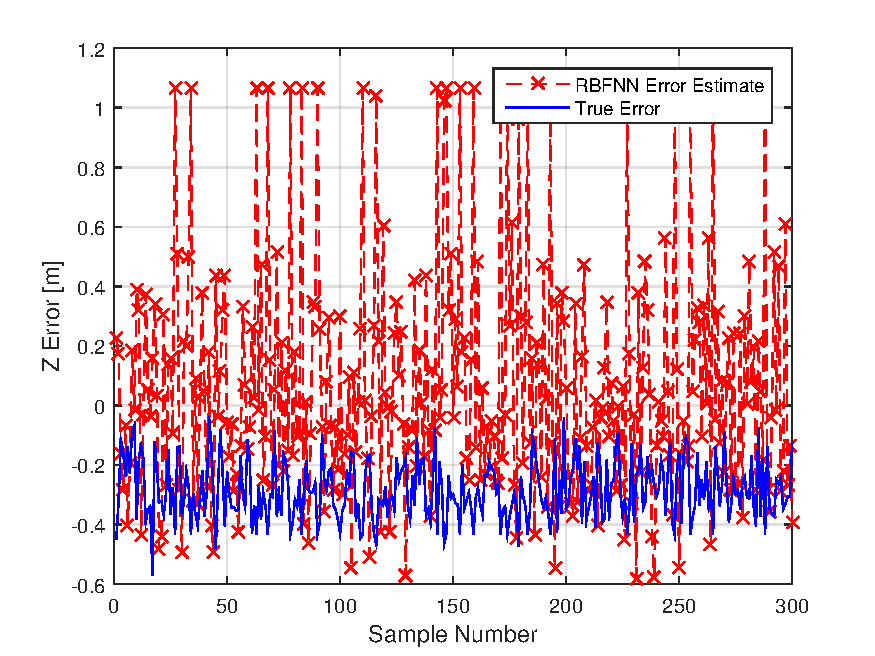
\includegraphics[width=\textwidth]{figures/chapter4/z_valid}
    \caption{}
  \end{subfigure}
~
  \begin{subfigure}{0.3\textwidth}
    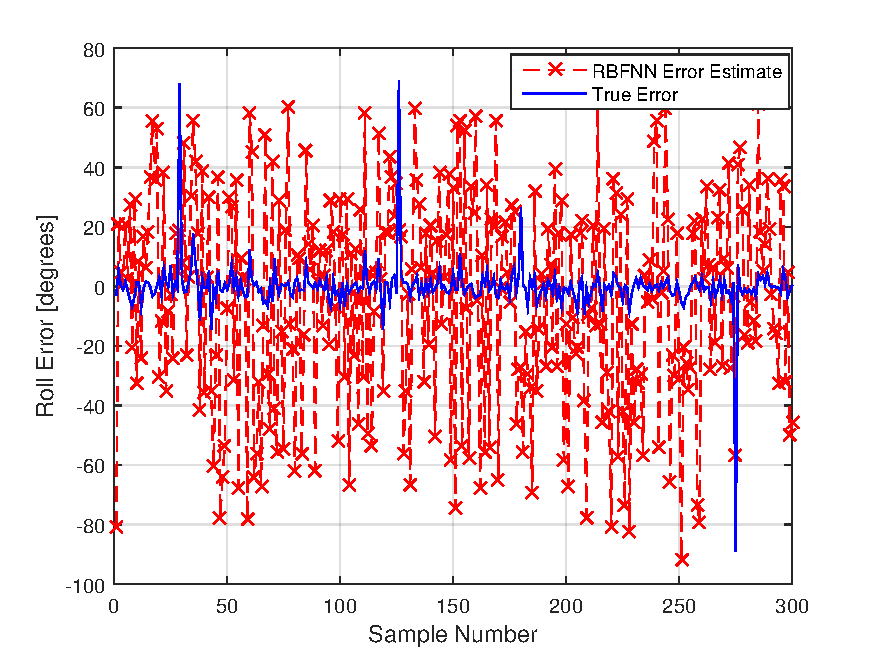
\includegraphics[width=\textwidth]{figures/chapter4/roll_valid}
    \caption{}
  \end{subfigure}
~
  \begin{subfigure}{0.3\textwidth}
    \includegraphics[width=\textwidth]{figures/chapter4/pitch_valid}
    \caption{}
  \end{subfigure}
~
  \begin{subfigure}{0.3\textwidth}
    \includegraphics[width=\textwidth]{figures/chapter4/yaw_valid}
    \caption{}
  \end{subfigure}
  \caption[The output of the RBFNN with the validation set input.]{A plot of the output for the different dimensions of the RBFNN when used with the validation data set.}
  \label{fig:chap4-rbf-valid}
\end{figure*}

\section{Conclusion}

In this chapter, a machine learning model was designed to model and predict the complex and dimensionally dependant error data of the CVS.\@ A radial basis function neural network was selected to do this: it takes a six-dimensional pose measurement vector from the CVS and outputs the corresponding measurement error for the input sample. The network was trained and validated by two different data sets from the same measurement test and produces a mean square error of 3.0 for the validation set, indicating a good fit. 

The trained network is now ready to predict the measurement error for the CVS with pose measurement data generated by a quadcopter in flight. This data can then be used to determine the pose estimation accuracy of a drone in flight. 


%\chapter{Quadcopter Test}
\label{chap5}

\section{Introduction}

The main objective of this research project is to determine the pose estimation accuracy of an airborne quadcopter in the outdoors. This can be done by comparing a quadcopter's on-board pose estimate with the pose measurement of an external measurement tool or device.  

In Chapter~\ref{chap3} a computer vision pose measurement system (CVS) was designed and tested and its pose measurement error was determined. It was found that the measurement data produced by the CVS is complex, high dimensional and interdimensionally dependant, as showed by the covariance matrix of Equation~\ref{eq:covariance-matrix}. This makes it hard to estimate the measurement error for any given pose measurement vector produced by the CVS.\@ 

Neural networks are known to be able to detect underlying relationships in the data, if properly designed and trained. In Chapter~\ref{chap4} a radial basis function neural network (RBFNN) was trained to be able to do this, since they have been proven to work well with complex, noisy and non-linear data. The accuracy of the trained RBFNN was verified by an additional data set and is ready to be used in a real test. 

The trained RBFNN was used with data gathered from a test flight from a quadcopter. This chapter sets out to discuss the design and details of the flight tests that were conducted, including the testing procedure, conditions and data processing. Then the results are presented and discussed, followed by a brief discussion on the data and results gathered thus far. 

\section{Test Design and Procedure}

\subsection{Introduction}

Some work was done to ensure that the flight tests were performed where it would produce meaningful results without posing a risk to the safety of bystanders and other equipment. This section discusses the planning that went into the test, as well as the equipment that was used, describes the test location and the test procedure, as well as the data processing.  

\subsection{Test Design}

\subsubsection{Equipment}

The equipment and facilities that were required and used for the flight tests are as follows:

\begin{itemize}
    \item CVS camera and laptop.
    \item Suncopter quadcopter.
    \item Certified unmanned aerial vehicle pilot.
    \item Calibration board.
    \item Isolated testing site. 
\end{itemize}

The details of the CVS are discussed in Chapter~\ref{chap3}. It consists of a camera, which captures the image data, and a laptop which records and processes the data. A certified unmanned aerial vehicle pilot was used for safety reasons, since the quadcopter will be flown in close proximity to people and other equipment. The calibration board is used in conjunction with the CVS to provide the pose data of the quadcopter. Here, the calibration board is an ISO A3-sized\footnote{$\SI{297}{\mm}\times\SI{432}{\mm}$}, $6\times5$ square chessboard pattern calibration board. 

The Suncopter quadcopter is a custom-built quadcopter for the Solar and Thermal Energy Research Group's (STERG) research purposes. It is FISIESE SPECS EN MODEL NR EN VERWYS NA SPEC SHEET\@.

\subsubsection{Location}

The flight tests were conducted at the Mariendahl experimental farm owned and operated by Stellenbosch University (SU). It is also the location of the Solar and Thermal Energy Research Group's (STERG) Helio100 central receiver concentrated solar power (CSP) project. The exact location is in an empty grass field relatively far away from any roadways and other buildings. The soil in the field is soft and uneven, which was taken into account during the tests and the data processing. 

\subsubsection{Test Conditions and Layout}

The flight tests were conducted on the 26$^{th}$ of June, 2015 at the Helio100 test site at Mariendahl. The weather conditions were close to ideal with very little wind, clear skies and a moderate temperature. The test was conducted at 10AM and the there was still significant condensation present on the ground. See Appendix MEME for a more detailed weather and wind report recorded on site.

For the test, video data of the Suncopter with a calibration board attached to its underside was recorded, where the pose data will be extracted off-line after the tests have been completed. The issue of turbulence introduced by a quadcopter flying too close to the ground was considered, since it can negatively affect its flight performance. A general rule of thumb to prevent ground effects from influencing a quadcopter's flight, as advised by~\cite{basson-flight-test}, is to fly a quadcopter the length of one of its props from the ground. The CVS's camera was placed on top of a $\SI{2}{\m}$ post, which is significantly higher than the diameter of the Suncopter's props, eliminating ground effects from the flight tests.

A certified pilot was employed during the test. His responsibility was to perform the manual piloting tasks, such as positioning the Suncopter and switching modes, as well as taking over the piloting of the Suncopter and safely land it in case the flight stability is compromised and a catastrophic failure was likely to occur. This was done in order to guarantee the safety of the equipment and on-site personnel. 

\subsection{Test Procedure}

For each flight test, the SunKopter was manually positioned above the centre of the CVS's camera on the post and set to \emph{loiter} mode. In this mode, the Suncopter will attempt to hold the altitude, position and yaw angle it had when it was set to \emph{loiter} mode, while remaining stable, meaning that the Suncopter will attempt to hold a roll and pitch angle of $\ang{0}$. 

It has been established in Chapter~\ref{chap3} that the pose measurement data from the CVS is highly interdimensionally dependant, which implies that the accuracy of the pose measurement will depend on the Suncopter's current pose relative to the CVS's camera. As a consequence of this, it was decided that several flight tests would be conducted, each with a slightly different distance or yaw angle relative to the CVS's camera. 

Distances of $\SI{1}{\m}$ and $\SI{2}{\m}$ from the camera were used. During preliminary flight tests, it was found that with distances greater than $\SI{2}{\m}$ from the camera, the CVS's camera started losing sight of the corners on the calibration board and struggled to detect and extract the corner coordinate data from the calibration board, making it impossible to perform the pose estimation. Furthermore, given that a quadcopter is symmetric about both of its axes, the yaw angles for the flight tests were set to $\ang{0}$, $\ang{22.5}$ and $\ang{45}$. 

Two sets of data was recorded during the flight test: one from the CVS and another from the on-board sensor suite of the Suncopter, which provides orientation and translation data. These two data sets will eventually allow the on-board pose estimation accuracy of the Suncopter to be determined. 

\subsection{Data Processing}

\subsubsection{Introduction}

After the video data of the Suncopter with the calibration board attached was recorded, the data processing stage could begin. There are four different processing phases. They are the pose extraction from the video data, synchronising the data to a common time frame, data recentering around a common centre, and finally determining the pose estimation accuracy of the Suncopter. Each of these phases are discussed in this section. 

\subsubsection{Pose Data Extraction}

The first step in the data processing phase is to extract the pose data of the calibration board, and by extension the Suncopter to which it was attached. This was done by using the process discussed in Chapter~\ref{chap2}, where OpenCV's chessboard corner detector and PnP problem solver were used to extract six-dimensional pose information of a chessboard pattern calibration board. This process is fairly automated, however the output from the PnP solver still required some conditioning.

The coordinate system for the corner detector and PnP solver used was specified in square units, i.e.\ a $5\times6$ square chessboard would have dimensions of $5\times6$ units. This required the position vector to be transformed back to SI units by multiplying the PnP solver's output by $0.05$, since each square on the chessboard is $\SI{5}{\cm}\times\SI{5}{\cm}$. Similarly, the orientation vector is output in radians, which was converted to degrees. 

\subsubsection{Data Synchronisation}

The CVS's camera captures video data at 30 frames per second, while the Pixhawk on the Suncopter sends data to the ground control station at a frequency of 200Hz, making it necessary to change the time scale of either data set to match one another. The Pixhawk's data packets contain various parameters, such as the battery voltage and altitude, but only the position and orientation data sets are of interest here. However, this data is not sent with every data package coming from the Pixhawk and do not necessarily arrive together either. It is therefore necessary to synchronise the position and orientation data received from the Pixhawk.

To synchronise the data, a zero-order-hold was applied to each data set by using the timestamps from each sample coming from the Suncopter. What this means is that the value of each sample is held constant until it is updated by the next sample. Furthermore, the CVS's pose data was downsampled by selecting a sample from the set that coincides with the timestamps from the Suncopter's pose data set. 

\subsubsection{Data Centering}
\label{sec:chap5-data-centring}

After the pose data has been extracted from the video data, the CVS and Suncopter's pose estimates must be recentred around a common axis system. The CVS's axis system is centred around its camera centre, while the Suncopter's pose data is centred around the point where it is launched from. Therefore, to be able to compare the two sets of data, the constant offset vector between the axis systems must be determined. The axis systems and offset vector is shown in Figure~\ref{fig:chap5-flight-test-schem}.

\begin{figure}
  \centering
  \includegraphics[width=0.8\textwidth]{figures/chapter5/test_flight_schem}
  \caption[Shematic of the test flight layout.]{Schematic of the test flight, the quadcopter and CVS's respective axis systems and the offset vector between them.}
\label{fig:chap5-flight-test-schem}
\end{figure}

Furthermore, any angular offset for the CVS camera or the Suncopter due to uneven ground conditions or camera placement, is also included in the offset vector. This makes the offset vector a six-dimensional position and orientation vector. The offset vector is a constant value and is related to the quadcopter and CVS's pose estimate by the relation given in Equation~\ref{eq:chap5-pose-offset}, where $\bm{P}$ is a six-dimensional pose vector. 

\begin{equation}
  \label{eq:chap5-pose-offset}
  \bm{P}_{quadcopter} = \bm{P}_{cvs} + \bm{P}_{of\!fset}
\end{equation}

In Equation~\ref{eq:chap5-pose-offset}, the $\bm{P}_{of\!fset}$ term is the unknown term. The pose data contained within the $\bm{P}_{quadcopter}$ and $\bm{P}_{cvs}$ terms contains noise in each sample, which requires that an optimisation procedure be used to find a offset vector that best relates the two sets of pose data. For the optimisation procedure, the cost function and error term in Equation~\ref{eq:chap5-err-func} was minimised, where the error vector $\bm{e}$ is a function of $\bm{P}_{of\!fset}$ and is given by Equation~\ref{eq:chap5-err-term}. 

\begin{equation}
  \label{eq:chap5-err-func}
  \text{Cost Function} = \min_{\bm{e}}\sqrt{\displaystyle\sum_{i=1}^{n} \bm{e}(\bm{P}_{of\!fset})_i^2}
\end{equation}

\begin{equation}
  \label{eq:chap5-err-term}
  \bm{e} = \bm{P}_{cvs} + \bm{P}_{of\!fset} - \bm{P}_{quadcopter}
\end{equation}

The minimisation was done using the \emph{minimize} function from the SciPy\footnote{SciPy v0.13.3} library for the Python language and makes use of the \emph{BFGS} quasi-Newton method described by~\cite{nocedal2006numerical}. 

\subsubsection{Determining the Pose Estimation Error}

With the two data sets now directly relatable, the pose estimation error of a quadcopter in flight can now be determined by using the radial basis function neural network (RBFNN) discussed in Chapter~\ref{chap4} and the two sets of pose data recorded during the flight tests.  

The input to the network is the CVS's recorded pose data. The network then outputs the expected measurement error for every sample, allowing a measurement error band to be drawn around the CVS's data. This error band can then be used to determine if the quadcopter or the CVS's pose estimates are more accurate: when the quadcopter's estimate falls within the error band, it can be assumed that the quadcopter's pose estimate is more accurate for that sample than the CVS's is, while the opposite holds true if it falls outside the error band. It can then be determined which of the two systems produce, on average, the most accurate pose measurements. However, if it is found that the quadcopter's pose estimate is more accurate, one might be liable to ask if the CVS is still necessary.

Up to this point, any measure of the error in a quadcopter's pose estimation has been unavailable to outdoor quadcopters, except their on-board pose estimates which cannot be used to determine their own accuracy. This means that even if it is found that the quadcopter's pose estimate is more accurate than the CVS's, the CVS pose data will still provide a worst-case measure of the quadcopter's pose estimate, which was not available previously. 

The outcome of this comparison may lead to one of the following two outcomes. If the quadcopter's pose estimate is more accurate than the CVS's, then the pose measurement error of the CVS can be taken as a quadcopter's worst-case pose measurement error, where the quadcopter's pose estimate will always be at least as accurate as, but likely better than the CVS's. Conversely, if it is found that the CVS produces better pose measures, then the quadcopter's pose estimation error will be given by the difference between the CVS and quadcopter's pose data. 

\section{Results}

\subsection{Offset Vector}

Using the procedure described in Section~\ref{sec:chap5-data-centring}, the optimal offset vector relating the quadcopter and CVS's axis systems is given in Equation~\ref{eq:chap5-offset-result}. 

\begin{equation}
  \label{eq:chap5-offset-result}
  \bm{P}_{of\!fset} = 
  \begin{bmatrix}
    \SI{-6.61}{\m} & \SI{-0.834}{\m} & \SI{-4.17}{\m} & \ang{6.15} & \ang{62.7} & \ang{-185} \\
  \end{bmatrix}^T
\end{equation}

The position values roughly coincide with the conditions that were recorded on site: the SunKopter was launched some distance from the CVS equipment for safety reasons. Due to uneven ground conditions at the testing site, the launch site was also slanted and located below the post on which the CVS's camera was placed. Thus, from a sanity check point of view, the offset that the optimisation procedure produced looks to be the correct one. 

\subsection{Pose Estimation Error}

Several different flight tests were conducted with different flight conditions. However, for convenience, only the results from the $\SI{1}{\m}$ altitude and $\ang{0}$ yaw case are presented and discussed. There is nothing special about this case and the data results from all the flight tests produce roughly the same results.  

Before the flight test data was fed to the RBFNN, it was first checked that the test data falls within the training data limits. This is done to ensure that the RBFNN is not exposed to data for which its output will be inaccurate, which it will be if it was not trained to handle data in that range. Figure~\ref{fig:chap5-ts-tr-scatter} shows scatter plots for the test and training data dimensions and shows that the test data falls comfortably within the training data set. 

\begin{figure*}
  \centering
  \begin{subfigure}{0.9\textwidth}
    \includegraphics[clip, trim = 120 40 120 0, width=\textwidth]{figures/chapter5/ts_v_tr_pos}
    \caption{Position data.}
  \end{subfigure}
  ~
  \begin{subfigure}{0.9\textwidth}
    \includegraphics[clip, trim = 120 40 120 0, width=\textwidth]{figures/chapter5/ts_v_tr_orient}
    \caption{Orientation data.}
  \end{subfigure}
  \caption[Scatter plots of flight data vs.\ training data. ]{Scatter plots showing that the flight test data falls within the training limits. }
  \label{fig:chap5-ts-tr-scatter}
\end{figure*}

The results for the flight test are presented in Figure~\ref{fig:chap5-results}. Here, six figures are given which plot the six different pose dimensions. Each plot contains the Suncopter's pose estimate, as well as the expected measurement error margin for the CVS, as given by the RBFNN.\@ It can be observed from the plots for the $z$ and yaw dimensions that they consistently hover around the flight configuration's set point of $\SI{1}{\m}$ and $\ang{0}$, providing a degree of sanity to the measurements. 
  
\begin{figure*}
  \centering
  \begin{subfigure}{0.45\textwidth}
    \includegraphics[clip, trim = 150 0 120 0, width=\textwidth]{figures/chapter5/x}
    \caption{$x$}
  \end{subfigure}
  \begin{subfigure}{0.45\textwidth}
    \includegraphics[clip, trim = 150 0 120 0, width=\textwidth]{figures/chapter5/roll}
    \caption{Roll}
  \end{subfigure}
  \begin{subfigure}{0.45\textwidth}
    \includegraphics[clip, trim = 150 0 120 0, width=\textwidth]{figures/chapter5/y}
    \caption{$y$}
  \end{subfigure}
  \begin{subfigure}{0.45\textwidth}
    \includegraphics[clip, trim = 150 0 120 0, width=\textwidth]{figures/chapter5/pitch}
    \caption{Pitch}
  \end{subfigure}
  \begin{subfigure}{0.45\textwidth}
    \includegraphics[clip, trim = 150 0 120 0, width=\textwidth]{figures/chapter5/z}
    \caption{$z$}
  \end{subfigure}
  \begin{subfigure}{0.45\textwidth}
    \includegraphics[clip, trim = 150 0 120 0, width=\textwidth]{figures/chapter5/yaw}
    \caption{Yaw}
  \end{subfigure}
  \caption[Plots of the Suncopter's flight and measurement errors.]{Plots of the Suncopter's pose estimate with the error margins from of the CVS's pose measurement. }
  \label{fig:chap5-results}
\end{figure*}

The first important aspect to note of the plots in Figure~\ref{fig:chap5-results} is that the quadcopter's estimate largely falls within the error boundaries for the CVS's pose measurement. This implies that the pose estimate given by the quadcopter's sensor suite is more accurate then the CVS's measurements, especially with its orientation estimate, where the CVS has a large area of uncertainty. The RBFNN has been adequately trained in Chapter~\ref{chap4} and Figure~\ref{fig:chap5-ts-tr-scatter} shows that the test data falls within the training data limits, giving a degree of certainty that the quadcopter's true position falls within the extreme CVS pose measurement errors. It therefore follows that the measurement error of the CVS can be taken as a worst-case pose estimation error for the Suncopter. 

Second, there are sections in the CVS error estimate plots which are missing. The reason for this is that during the video recording, the calibration board went out of the CVS's camera's field of view or it could not detect enough of the corners due to bad lighting conditions or the board being to far from the camera, for example. These effects were somewhat remedied by adjusting the pose extractor to use an adaptive threshold filter on the video data and can permanently fixed by flying the quadcopter closer to the camera or ensuring that the board is well and evenly lit. 

\section{Conclusion}

In this chapter, the CVS and RBFNN was used to measure the pose of an airborne quadcopter in the outdoors and to find the quadcopter's pose estimation accuracy. It was found that the quadcopter's on-board pose estimate is more accurate than the CVS's.\@ However, the CVS's pose measurement error can still be used to provide a measure of how accurately the quadcopter can estimate its position, since its estimates will at worst be as good as the CVS's.\@ 

%\chapter{Conclusion}
\label{chap6}

\section{Introduction}

This research project set out to accomplish two things: find a reliable, accurate and cheap method to measure the six-dimensional pose of an object in the outdoors, and then to use that system to determine the pose estimation accuracy of an unmanned aerial vehicle (UAV) quadcopter in flight in the outdoors. The pose refers to a six-dimensional vector describing an object's position and orientation. 

Previous chapter in this paper have covered each aspect of the computer vision system design, testing and implementation process, as well as live testing with a quadcopter. This chapter will provide a brief summary of this paper, as well as the key findings and results. The significance of these findings to the existing body of knowledge is also discussed. Finally, the shortcomings of the findings and their potential solutions and future work is discussed. 

\section{Thesis Summary}

Chapter meme starts th e thesis document off with an introduction to the problem and motivates the reason why a new outdoor measurement system needs to be developed and what the potential benefits are to knowing how accurately a UAV can estimate its pose.  

A review of the current body of knowledge pertaining to the relevant aspects of this research project is given in Chapter meme. It was found that a significant amount of research has already been done in stabilising a UAV and having it hold its position in the air with different control strategies. Furthermore, it was established that the computer vision techniques and libraries available that can extract the pose data for an object from an image, are fairly well understood and widely researched. Finally, this chapter includes a brief review of the different machine learning techniques available that can be trained to make accurate predictions for a given input vector. The different techniques with their strengths and shortcomings are discussed.  

In Chapter meme, all of the design aspects of the computer vision system (CVS) is discussed, which include the hardware and software design as well as the measurement accuracy test and verification process. It was found that the complex nature of the CVS's measurement error necessitates a prediction algorithm to predict what the measurement error would be for any given input pose measurement vector from the CVS. 

Chapter meme is set out to discuss using a radial basis function neural network (RBFNN) to estimate the measurement error for the pose vector produced by the CVS. It discusses the training process used and how the trained network's estimation accuracy was was verified. A RBFNN was trained which produces an nacceptable level of error with its estimates and can be used with new pose measurement data.

Finally, Chapter meme is dedicated to discussing how the CVS and the RBFNN was used with a flight test with a real quadcopter.

\section{Findings and Contributions to Body of Knowledge}

The objectives of this research thesis are discussed in Chapter meme. They are stated here again for convenience and are as follows:

\begin{itemize}
  \item Design and implement an alternative outdoor pose measurement system.
  \item Determine the measurement accuracy of that pose measurement system.
  \item Use the computer vision system to determine the pose estimation accuracy of a quadcopter in flight. 
\end{itemize}

The main objective is to determine the pose estimation accuracy of a quadcopter in flight in an outdoor environment. To be able to do this, a new pose measurement tool needed to be employed that would work in the outdoors. To this end, a camera-based system was made that makes use of existing computer vision techniques to extract pose information from image data. However, before this system could be used to make real pose measurements, its accuracy first needed to be determined.

This was done by using a Vicon motion-tracking system, whose measurements provided a ground-truth baseline with which the CVS's pose measurements could be compared against. Consequently, the CVS's measurement error data was found to be complex and high-dimensional and highly interdimensionally dependant, as shown by the covariance matrix in Equation meme. This made it necassary to use a machine learning model to predict measurement error for any input pose measurement vector, since the measurement error is not constant and varies according to the current pose of the object relative to the CVS's camera. 

To perform the measurement error prediction, a RBFNN was selected based on its ability to work well with noisy input data and detect and characterise non-linear relationships between the input dimensions. This network was trained and validated with data gathered during the Vicon test and produces a normalised mean square error of meme for the training set and meme for the validations set. These small errors indicate that the network was trained well and overfitting did not occur. The trained RBFNN was then ready predict the measurement error for new pose measurement data.

With the CVS designed and ready to make measurements and the RBFNN trained and ready to determine the error in the CVS data, a real flight test could be conducted where the pose estimation accuracy of a quadcopter in flight was determined. For the 

\section{Shortcomings and Future Work}

\section{Conclusion}



				    
%==== Appendices ====================================================
\appendix
\appendixpage\relax
		  
%\include{contents/App-1}
%\include{contents/App-2}
%\include{contents/App-3}
	    
%==== Bibliography acro's & Index ===================================
\backmatter%
      
\bibliography{backmatter/bibliography}

\end{document}
